\documentclass[UTF8,zihao=-4]{ctexart}
\usepackage[a4paper,margin=1.85cm,headheight=26pt]{geometry}
\usepackage{graphicx}
\usepackage{booktabs}
\usepackage{longtable}
\usepackage{tabularx}
\usepackage{xcolor}
\usepackage{hyperref}
\usepackage{fancyhdr}
\usepackage{enumitem}
\usepackage{titlesec}
\usepackage{array}
\usepackage{float}
\usepackage{caption}
\usepackage{multicol}
\graphicspath{{docs/}}
\definecolor{nexusInk}{HTML}{172033}
\definecolor{nexusMuted}{HTML}{64748B}
\definecolor{nexusTeal}{HTML}{0F766E}
\definecolor{nexusGold}{HTML}{9A6A18}
\definecolor{nexusLine}{HTML}{CBD5E1}
\definecolor{nexusPanel}{HTML}{F7F9FB}
\hypersetup{colorlinks=true,linkcolor=nexusTeal,urlcolor=nexusTeal}
\pagestyle{fancy}
\fancyhf{}
\lhead{\textcolor{nexusMuted}{NEXUS Prime 制造业 ERP}}
\rhead{\textcolor{nexusMuted}{全量交付报告}}
\cfoot{\textcolor{nexusMuted}{\thepage}}
\renewcommand{\headrulewidth}{0.3pt}
\renewcommand{\headrule}{\hbox to\headwidth{\color{nexusLine}\leaders\hrule height \headrulewidth\hfill}}
\titleformat{\section}{\Large\bfseries\color{nexusInk}}{\thesection}{0.7em}{}[\vspace{0.15em}{\color{nexusTeal}\titlerule[0.8pt]}]
\titleformat{\subsection}{\large\bfseries\color{nexusInk}}{\thesubsection}{0.7em}{}
\setlist[itemize]{leftmargin=2em,itemsep=0.18em,topsep=0.25em}
\renewcommand{\arraystretch}{1.2}
\emergencystretch=5em
\sloppy
\newcommand{\code}[1]{{\small\url{#1}}}
\newcommand{\tightpara}[1]{{\small #1\par}}
\begin{document}
\begin{titlepage}
  \centering
  \vspace*{1.1cm}
  {\Huge\bfseries\color{nexusInk} NEXUS Prime\par}
  \vspace{0.3cm}
  {\Large\bfseries\color{nexusTeal} 制造业经营管理 ERP 全量交付报告\par}
  \vspace{0.45cm}
  {\large Angular 21 + Flask REST API + SQLAlchemy + Tencent CloudBase\par}
  \vfill
  \begin{tabularx}{0.96\textwidth}{>{\bfseries}lX}
    前端地址 & \code{https://constantine-d3gjhwmtz0336c36a-1448158108.tcloudbaseapp.com/nexus-prime-fulldata-06292135-44aed6a/} \\
    后端 API & \code{https://nexus-api-fulldata-06292135-44aed6a-276095-6-1448158108.sh.run.tcloudbase.com/api/v1} \\
    完整数据资产 & \code{https://constantine-d3gjhwmtz0336c36a-1448158108.tcloudbaseapp.com/nexus-data/nexus_prime_full_06292108.db.gz} \\
    演示账号 & \code{admin@nexus.com / admin123}; \code{user00001@nexus.com / password123} \\
    报告日期 & 2026-06-29 \\
  \end{tabularx}
  \vfill
  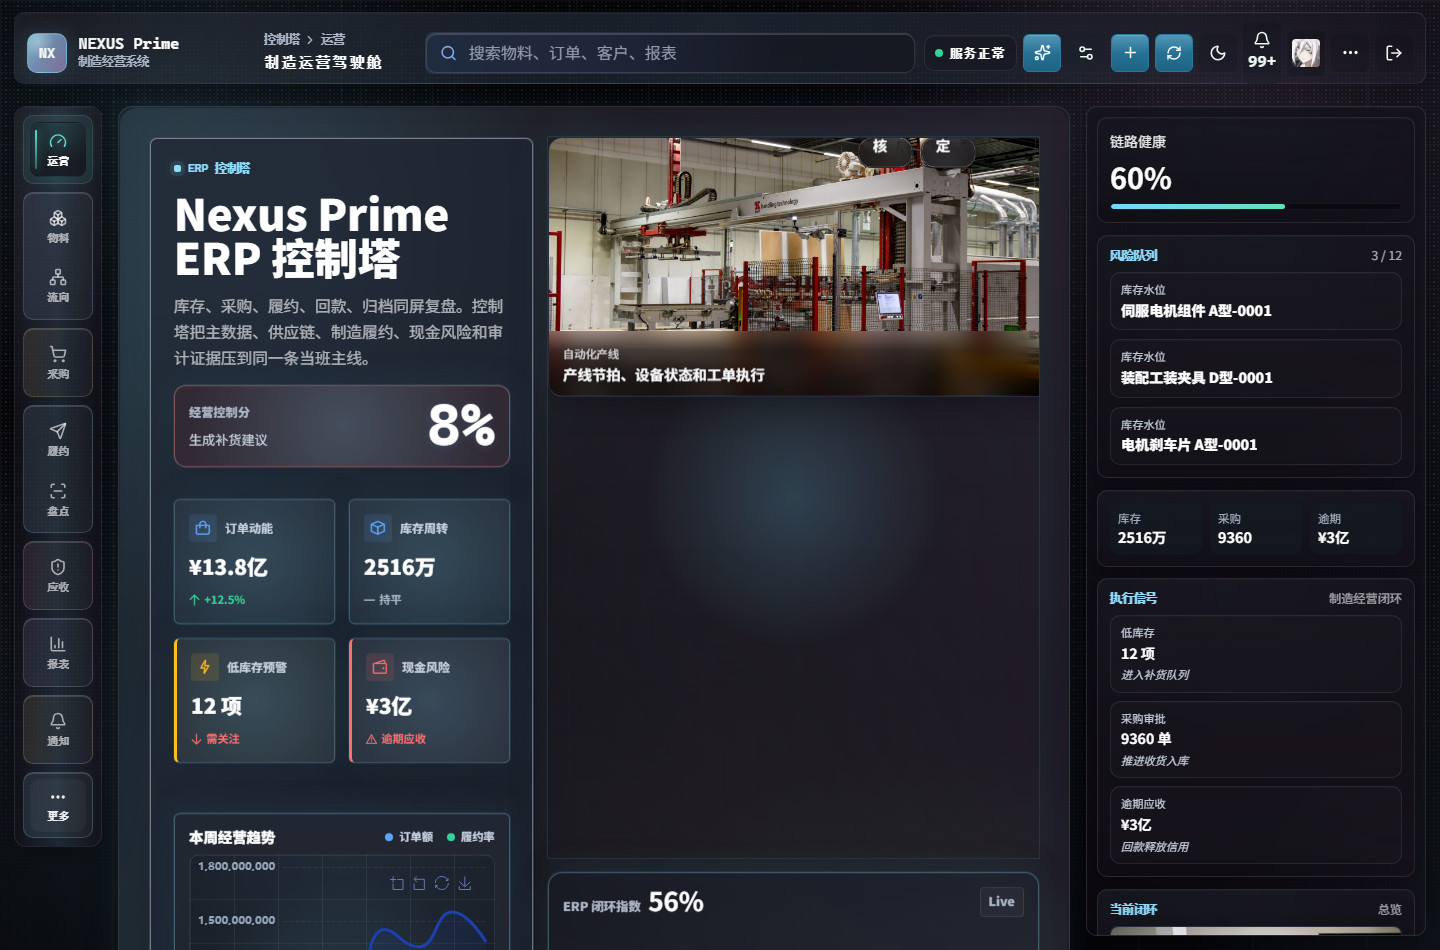
\includegraphics[width=0.92\textwidth,height=0.46\textheight,keepaspectratio]{images/final/pages/desktop-dark-cockpit-overview.png}
  \vfill
\end{titlepage}
\tableofcontents
\clearpage
\section{线上部署和完整数据}
\begin{longtable}{p{0.24\textwidth}p{0.66\textwidth}}
\toprule
项目 & 结果 \\
\midrule
\endhead
前端可分享地址 & \code{https://constantine-d3gjhwmtz0336c36a-1448158108.tcloudbaseapp.com/nexus-prime-fulldata-06292135-44aed6a/} \\
后端 API Base & \code{https://nexus-api-fulldata-06292135-44aed6a-276095-6-1448158108.sh.run.tcloudbase.com/api/v1} \\
CloudBase 环境 & \code{constantine-d3gjhwmtz0336c36a} \\
后端服务 & \code{nexus-api-fulldata-06292135-44aed6a} \\
完整库资产 & \code{https://constantine-d3gjhwmtz0336c36a-1448158108.tcloudbaseapp.com/nexus-data/nexus_prime_full_06292108.db.gz} \\
管理员登录 & \code{admin@nexus.com / admin123}, HTTP 200 \\
普通用户登录 & \code{user00001@nexus.com / password123}, HTTP 200 \\
\bottomrule
\end{longtable}

本次上线已经使用完整本地演示数据库，不再使用小型演示库。完整 SQLite 原始文件约 244MB，压缩后约 46MB。部署过程先把压缩库上传到 CloudBase 静态托管，再由 CloudRun 启动脚本下载、解压、写锁验证、quick check 校验和最小数据量断言，最后再启动 Flask API。

\begingroup
\small
\renewcommand{\arraystretch}{1.08}
\begin{tabularx}{\textwidth}{p{0.34\textwidth}r p{0.34\textwidth}r}
\toprule
表和含义 & 云端数量 & 表和含义 & 云端数量 \\
\midrule
\code{auth_users}\newline {\footnotesize 用户账号} & 15001 & \code{biz_products}\newline {\footnotesize 物料商品} & 57609 \\
\code{biz_partners}\newline {\footnotesize 客户供应商伙伴} & 25200 & \code{trade_orders}\newline {\footnotesize 销售订单} & 100803 \\
\code{trade_order_items}\newline {\footnotesize 销售明细} & 201603 & \code{purchase_orders}\newline {\footnotesize 采购订单} & 46803 \\
\code{purchase_order_items}\newline {\footnotesize 采购明细} & 93603 & \code{finance_receivables}\newline {\footnotesize 应收账款} & 80640 \\
\code{finance_payments}\newline {\footnotesize 收款记录} & 70560 & \code{stock_quantities}\newline {\footnotesize 库存数量} & 111360 \\
\code{stock_logs}\newline {\footnotesize 库存日志} & 111360 & \code{sys_notifications}\newline {\footnotesize 系统通知} & 32431 \\
\code{sys_audit_logs}\newline {\footnotesize 审计日志} & 7694 & \code{cms_articles}\newline {\footnotesize 公告知识文章} & 16200 \\
\code{generated_reports}\newline {\footnotesize 生成报表} & 16200 & & \\
\bottomrule
\end{tabularx}
\endgroup

\vspace{0.5em}
\begin{tabularx}{\textwidth}{>{\bfseries}p{0.18\textwidth}X}
\toprule
验证维度 & 证据 \\
\midrule
服务健康 & \code{/api/v1/health/ready} 返回 HTTP 200，说明 CloudRun 服务和运行数据库可访问。 \\
登录链路 & 管理员和普通用户账号均已登录成功，说明 Cookie、CSRF、跨域和用户恢复链路可用。 \\
完整数据 & 诊断接口返回 15001 个用户、100803 张销售订单和完整库存、采购、财务、报表数据，证明线上不是空库。 \\
启动保护 & \code{bootstrap_sqlite.py} 下载压缩库后执行写锁测试、\code{pragma quick_check} 和最小数据量断言，避免空库误上线。 \\
前端配置 & 前端构建写入线上 API Base，CloudBase 静态托管页面直接请求 CloudRun API，不再依赖本地地址。 \\
分享交付 & 前端地址、后端 API、完整数据库资产和演示账号都放在报告首页，方便评审直接访问。 \\
\bottomrule
\end{tabularx}
\vspace{0.65em}
\begin{tabularx}{\textwidth}{>{\bfseries}p{0.18\textwidth}X}
\toprule
验收结论 & 说明 \\
\midrule
数据完整 & 用户、商品、伙伴、销售、采购、库存、财务、通知、审计、文章和报表都达到完整库规模。 \\
链路闭合 & 首页进入登录，登录后进入 \code{/app/**}，再由 Dock、顶部栏和资源操作台管理全部业务入口。 \\
可演示性 & 管理员账号用于系统、权限、审计和全局数据演示；普通账号用于常规业务角色演示。 \\
可追溯性 & 后端权限、审计日志、资源注册表和部署诊断共同支撑课程验收时的问题回溯。 \\
不改入口 & 首页、登录页、注册页只在报告里使用暗色截图，源码保持原样，避免入口视觉被额外改动影响验收。 \\
\bottomrule
\end{tabularx}

这一页的结论是：云端不是“能跑起来”的空壳，而是带着完整本地数据、完整认证链路和完整业务入口一起上线。对于评审来说，先看这页就能确认三个最关键的东西：系统可访问、数据完整、入口未被改坏。
\vspace{0.35em}
\clearpage
\section{架构设计和升级思路}
系统采用 Angular 21 SPA + Flask REST API + SQLAlchemy/Alembic 的前后端分离架构。首页、登录页和注册页保持原样，登录后的 \code{/app/**} 业务区统一进入 App Shell。

\begin{verbatim}
CloudBase Static Hosting
  Angular SPA / runtime-config.js
        | HTTPS + HttpOnly Cookie + CSRF
CloudBase CloudRun
  Flask /api/v1 / Auth / Policy / Audit / Domain Services
        | SQLAlchemy
SQLite full demo DB bootstrapped from CloudBase asset
\end{verbatim}

升级重点是把零散页面整理为一套 ERP 工作台。Dock 不再拉长，顶部栏统一搜索、面包屑、状态、主题、通知和头像。页面结构统一为上方真实图和关键图表，中部交互报表，下方表格、表单、增删查改和分页。大量无意义小方框被改成摘要、图表、表格和执行队列。

\begingroup
\small
\renewcommand{\arraystretch}{1.06}
\begin{tabularx}{\textwidth}{p{0.2\textwidth}X}
\toprule
升级重点 & 说明 \\
\midrule
导航逻辑统一 & 原来左侧 Dock、省略号、页面顶部卡片和页面内部跳转并行存在，用户会被迫在多套规则之间猜测入口。本轮把 `/app/**` 全部纳入 `navigation.ts` 和 App Shell，Dock 是一级业务流程，顶部栏是当前位置、搜索和全局动作，模块操作台是当前资源的增删查改。 \\
Dock 交互收敛 & Dock 删除按钮拉长动画，不再让按钮 hover 后挤占空间；所有入口按业务域分组展示，一行一个稳定按钮，图标、短标签、当前态和浮窗名称共同表达含义。这样既保留文字说明，也避免动画导致布局跳动。 \\
顶部栏合并 & 顶部栏从零散按钮升级为统一控制面。搜索栏负责跨物料、订单、客户、报表的命令搜索；头像区域只承担个人工作台和退出；主题切换只保留深色和亮色两个可理解状态；服务健康、通知和快捷创建都放在同一层级。 \\
页面结构统一 & 每个业务页面都遵循“真实图/关键图表在上，交互报表在中，表格、表单、分页和 CRUD 在下”的布局。运营页的设计理念被推广到库存、采购、销售、财务、AI、个人页和设置页，减少孤立方框和未利用空白。 \\
空间利用优化 & 大面积空白区域不再放无意义卡片，而是放交互报表、执行队列、图表说明、分页表格和当前模块操作台。每页控制长度，信息分层清晰，避免上下页显示不全和底部操作台被挤出视口。 \\
数据与部署兜底 & 云端不再使用小型演示库，而是上传本地完整库。启动脚本会验证用户数和销售订单数，避免迁移空库后前端看起来正常但数据缺失。报告也把云端数据量列出，便于验收。 \\
\bottomrule
\end{tabularx}
\endgroup

\vspace{0.55em}
这些升级共同解决三个问题：第一，路由入口只服从 Dock、顶部搜索和当前资源操作台三层结构；第二，页面视觉不再用大量孤立方框堆叠，而是把真实图、图表、表格和表单放到稳定位置；第三，数据和权限由后端兜底，前端负责把业务动作讲清楚，避免页面看起来能跳、实际上没有业务闭环。
\clearpage

\section{代码结构总览}
下面按运行链路说明关键代码。这里不是简单列文件名，而是说明为什么这些文件能支撑本次导航、主题、页面布局、资源操作台和云端完整数据上线。

\begin{longtable}{p{0.2\textwidth}p{0.28\textwidth}p{0.44\textwidth}}
\toprule
主题 & 文件 & 设计说明 \\
\midrule
\endhead
前端 API 总线 & \code{frontend/src/app/core/api.service.ts} & 统一封装 HttpClient、withCredentials、查询参数和 envelope 解包。页面组件不再散落拼接 URL，也不直接处理后端统一响应结构，从而降低每个业务页重复错误处理的概率。 \\
认证与会话恢复 & \code{frontend/src/app/core/auth.service.ts, auth.guard.ts, auth.interceptor.ts} & 登录结果写入 sessionStorage 和 CSRF 缓存，真正的会话凭据保留在 HttpOnly Cookie 中；刷新页面时 authGuard 会先检查 Cookie hint，再通过 /auth/me 恢复用户，避免误把可恢复会话踢回登录页。 \\
主题与偏好 & \code{frontend/src/app/core/theme.service.ts} & 主题源被收敛为 dark-cockpit 与 light-luxury 两个实际展示状态，写入 localStorage 与用户偏好；切换后同时更新 html class、data-theme 和 nexus-theme-change 事件，图表与组件可以同步刷新。 \\
导航壳层 & \code{frontend/src/app/shell/app-shell.component.ts} & 登录后页面统一进入 App Shell。它管理 Dock、顶部栏、搜索防抖、通知轮询、服务健康、路由 loading 和页面滚动复位，避免各页面自己实现一套壳层逻辑。 \\
左侧 Dock & \code{frontend/src/app/shell/app-dock.component.ts, frontend/src/app/core/navigation.ts} & Dock 数据来自统一导航模型，按运营、仓配、供应、履约、财务、分析、协作、安全、个人分组。按钮不再做拉长动画，采用稳定图标、短标签、当前态和文字浮窗。 \\
顶部导航 & \code{frontend/src/app/shell/app-topbar.component.ts} & 顶部栏合并品牌、面包屑、搜索、服务健康、快捷创建、AI、设置、主题、通知、头像与退出，避免页面上出现多套跳转规则并行。 \\
模块操作台 & \code{frontend/src/app/shell/resource-workbench.component.ts, frontend/src/app/core/resource-workflow.ts} & 对可 CRUD 的模块提供统一搜索、分页、详情、创建、编辑、删除、导出和领域动作配置。页面上方负责看业务态势，下方负责实际数据操作。 \\
后端认证权限 & \code{backend/app/api/auth\_routes.py, backend/app/platform/auth/decorators.py, backend/app/platform/policy/policy\_engine.py} & 后端集中处理登录、注册、CSRF、JWT、权限装饰器、管理员覆盖、资源权限、对象授权和字段过滤，前端展示权限不是最终安全边界。 \\
通用 CRUD & \code{backend/app/api/generic\_crud\_routes.py, backend/app/platform/crud/*} & 资源注册表统一接入列表、详情、搜索、创建、更新、删除、分页和审计。新增资源时优先注册资源配置，而不是复制一组相似接口。 \\
完整库启动 & \code{backend/scripts/bootstrap\_sqlite.py} & CloudRun 启动时读取 backend/.env，下载完整 SQLite 压缩库，解压到 /tmp/nexus-prime，执行写锁测试、pragma quick\_check 和最小数据量断言，防止空库误上线。 \\
腾讯云发布脚本 & \code{deploy/tencent-cloudbase-auto-deploy.ps1} & 脚本负责准备后端 CloudRun 源码、写入生产环境变量、构建前端、上传静态托管路径，并支持完整库引导参数与唯一版本后缀。 \\
\bottomrule
\end{longtable}
\clearpage

\section{组件职责矩阵}
这一页把运行链路拆成组件职责。它对应用户最关心的“为什么页面不会再乱跳”：入口保护、API、Shell、Dock、顶栏、资源操作台、后端授权和完整库启动各自只负责一层，页面组件不再重复实现导航和 CRUD 规则。

\begin{tabularx}{\textwidth}{p{0.2\textwidth}p{0.3\textwidth}X}
\toprule
层级 & 文件或组件 & 职责 \\
\midrule
运行配置 & \code{runtime-config.js} & 前端读取线上 API Base，不把敏感变量放到浏览器。 \\
认证守卫 & \code{auth.guard.ts} & 保护登录后路由，刷新时恢复 Cookie 会话。 \\
API 服务 & \code{api.service.ts} & 统一 withCredentials、路径、envelope 解包和错误处理。 \\
App Shell & \code{app-shell.component.ts} & 登录后壳层、搜索、通知、模块状态和页面容器。 \\
Dock & \code{app-dock.component.ts} & 统一核心流程入口，删除按钮拉长动画。 \\
顶栏 & \code{app-topbar.component.ts} & 搜索、主题、通知、头像和面包屑。 \\
后端认证 & \code{auth_routes.py}, \code{decorators.py} & 登录、CSRF、JWT、权限装饰器。 \\
策略引擎 & \code{policy_engine.py} & 管理员、权限、对象和字段级授权。 \\
完整库启动 & \code{bootstrap_sqlite.py} & 下载、解压、写锁、quick check 和数据量断言。 \\
\bottomrule
\end{tabularx}

\vspace{0.7em}
\begin{tabularx}{\textwidth}{>{\bfseries}p{0.2\textwidth}X}
\toprule
约束 & 落地方式 \\
\midrule
入口不改 & 首页、登录页、注册页源码保持不变，报告只使用暗色截图说明入口流程。 \\
跳转归一 & \code{navigation.ts} 作为 Dock、面包屑、当前模块和跳转关系的唯一业务地图。 \\
操作归一 & \code{resource-workbench.component.ts} 统一承载搜索、分页、表单、删除、导出和领域动作。 \\
视觉归一 & 页面上方展示真实图与关键图表，中部放交互报表，下方放 CRUD 操作台。 \\
数据兜底 & \code{bootstrap_sqlite.py} 校验完整数据规模，防止空库或裁剪库误上线。 \\
\bottomrule
\end{tabularx}
\clearpage
\section{完整 ER 图和数据模型}
\begin{figure}[H]
  \centering
  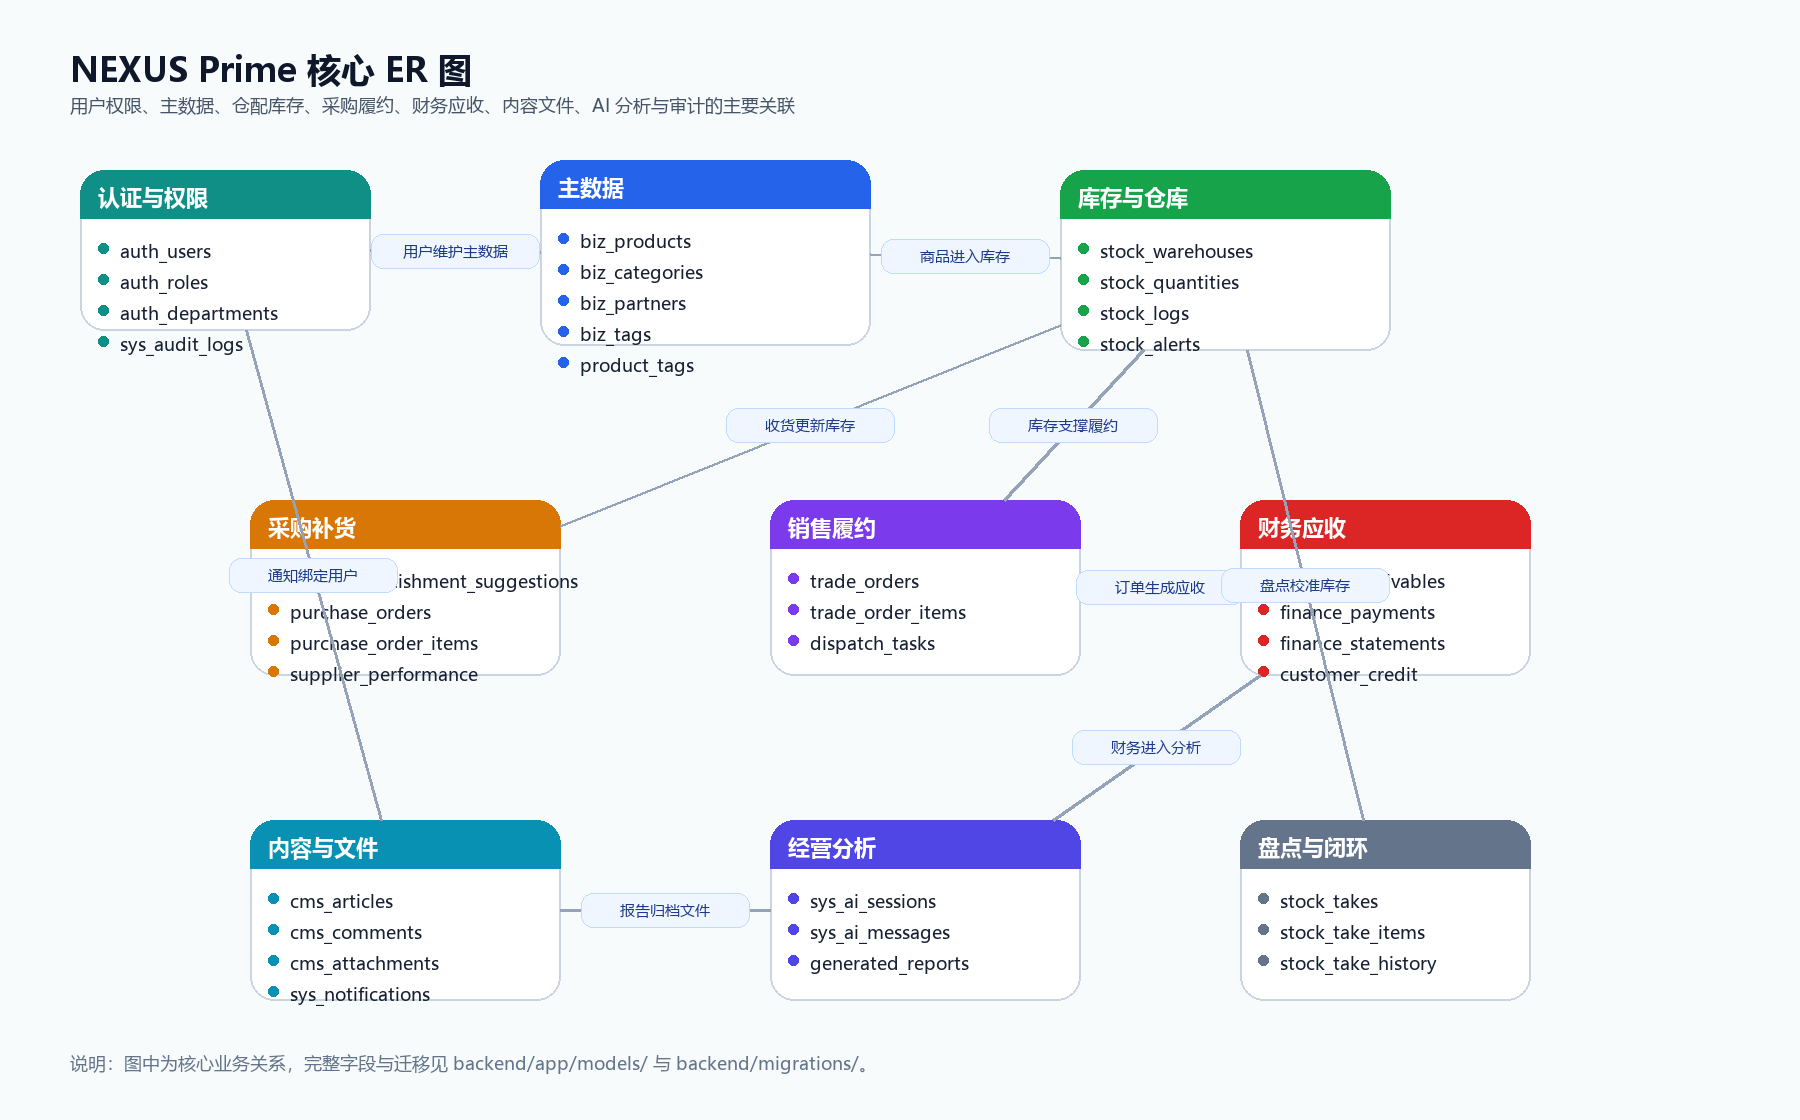
\includegraphics[width=\textwidth,height=0.72\textheight,keepaspectratio]{images/final/er-diagram.png}
  \caption{完整 ER 图}
\end{figure}
数据库按领域划分为身份权限、主数据、库存仓配、采购、销售履约、财务应收、盘点、工作流、内容文件、报表分析、通知审计、AI 会话和异步事件。关键关系包括：商品和仓库通过库存数量表关联；销售订单形成应收账款；应收账款通过收款记录核销；补货建议可转采购单；采购单、销售单和盘点单都有关联明细；用户动作进入审计日志。

\begin{tabularx}{\textwidth}{>{\bfseries}p{0.2\textwidth}X}
\toprule
领域 & ER 覆盖说明 \\
\midrule
身份权限 & 用户、角色、权限和部门决定谁能进入系统、看到哪些模块、执行哪些动作。 \\
主数据 & 商品、分类、标签、客户和供应商是采购、库存、销售、财务共同引用的事实源。 \\
库存采购 & 仓库、库存数量、库存流水、预警、补货建议和采购订单形成补货闭环。 \\
销售财务 & 客户、销售订单、订单明细、应收、收款、信用和合同形成履约回款闭环。 \\
工作流协作 & 流程实例、任务、日志、通知、文章、附件和报表把业务结果沉淀为协作证据。 \\
AI 分析 & AI 会话、消息、文档分块和行动草稿支撑经营问答、结构化诊断和后续执行。 \\
\bottomrule
\end{tabularx}
\clearpage
\section{身份权限与主数据 ER}
\begin{figure}[H]
  \centering
  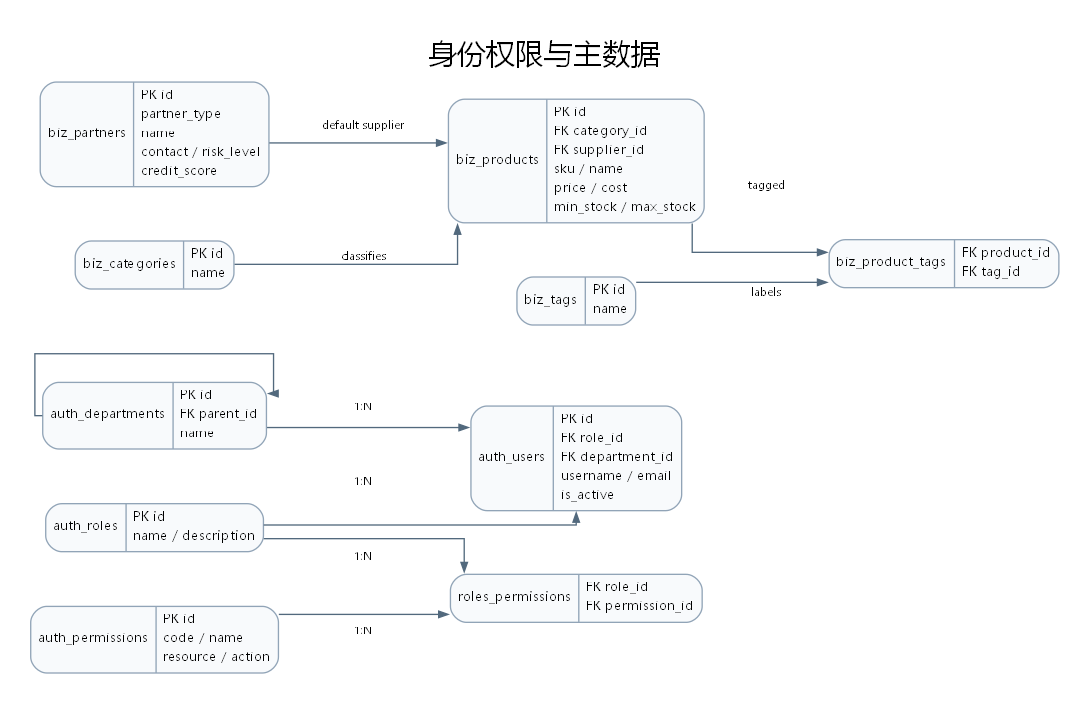
\includegraphics[width=\textwidth,height=0.66\textheight,keepaspectratio]{images/final/er-identity-master.png}
  \caption{身份权限与主数据 ER}
\end{figure}
该图覆盖账号、角色、权限、部门、客户供应商、物料分类、物料标签和商品主数据。身份权限决定谁能进入系统、能执行哪些动作；主数据则是采购、库存、销售、财务等后续交易的共同事实源。

这张分域图用于弥补全局 ER 图信息密度过高的问题。全局图负责展示系统全貌，分域图负责在课程讲解时逐个解释表、外键和业务闭环。
\clearpage
\section{库存仓配与采购补货 ER}
\begin{figure}[H]
  \centering
  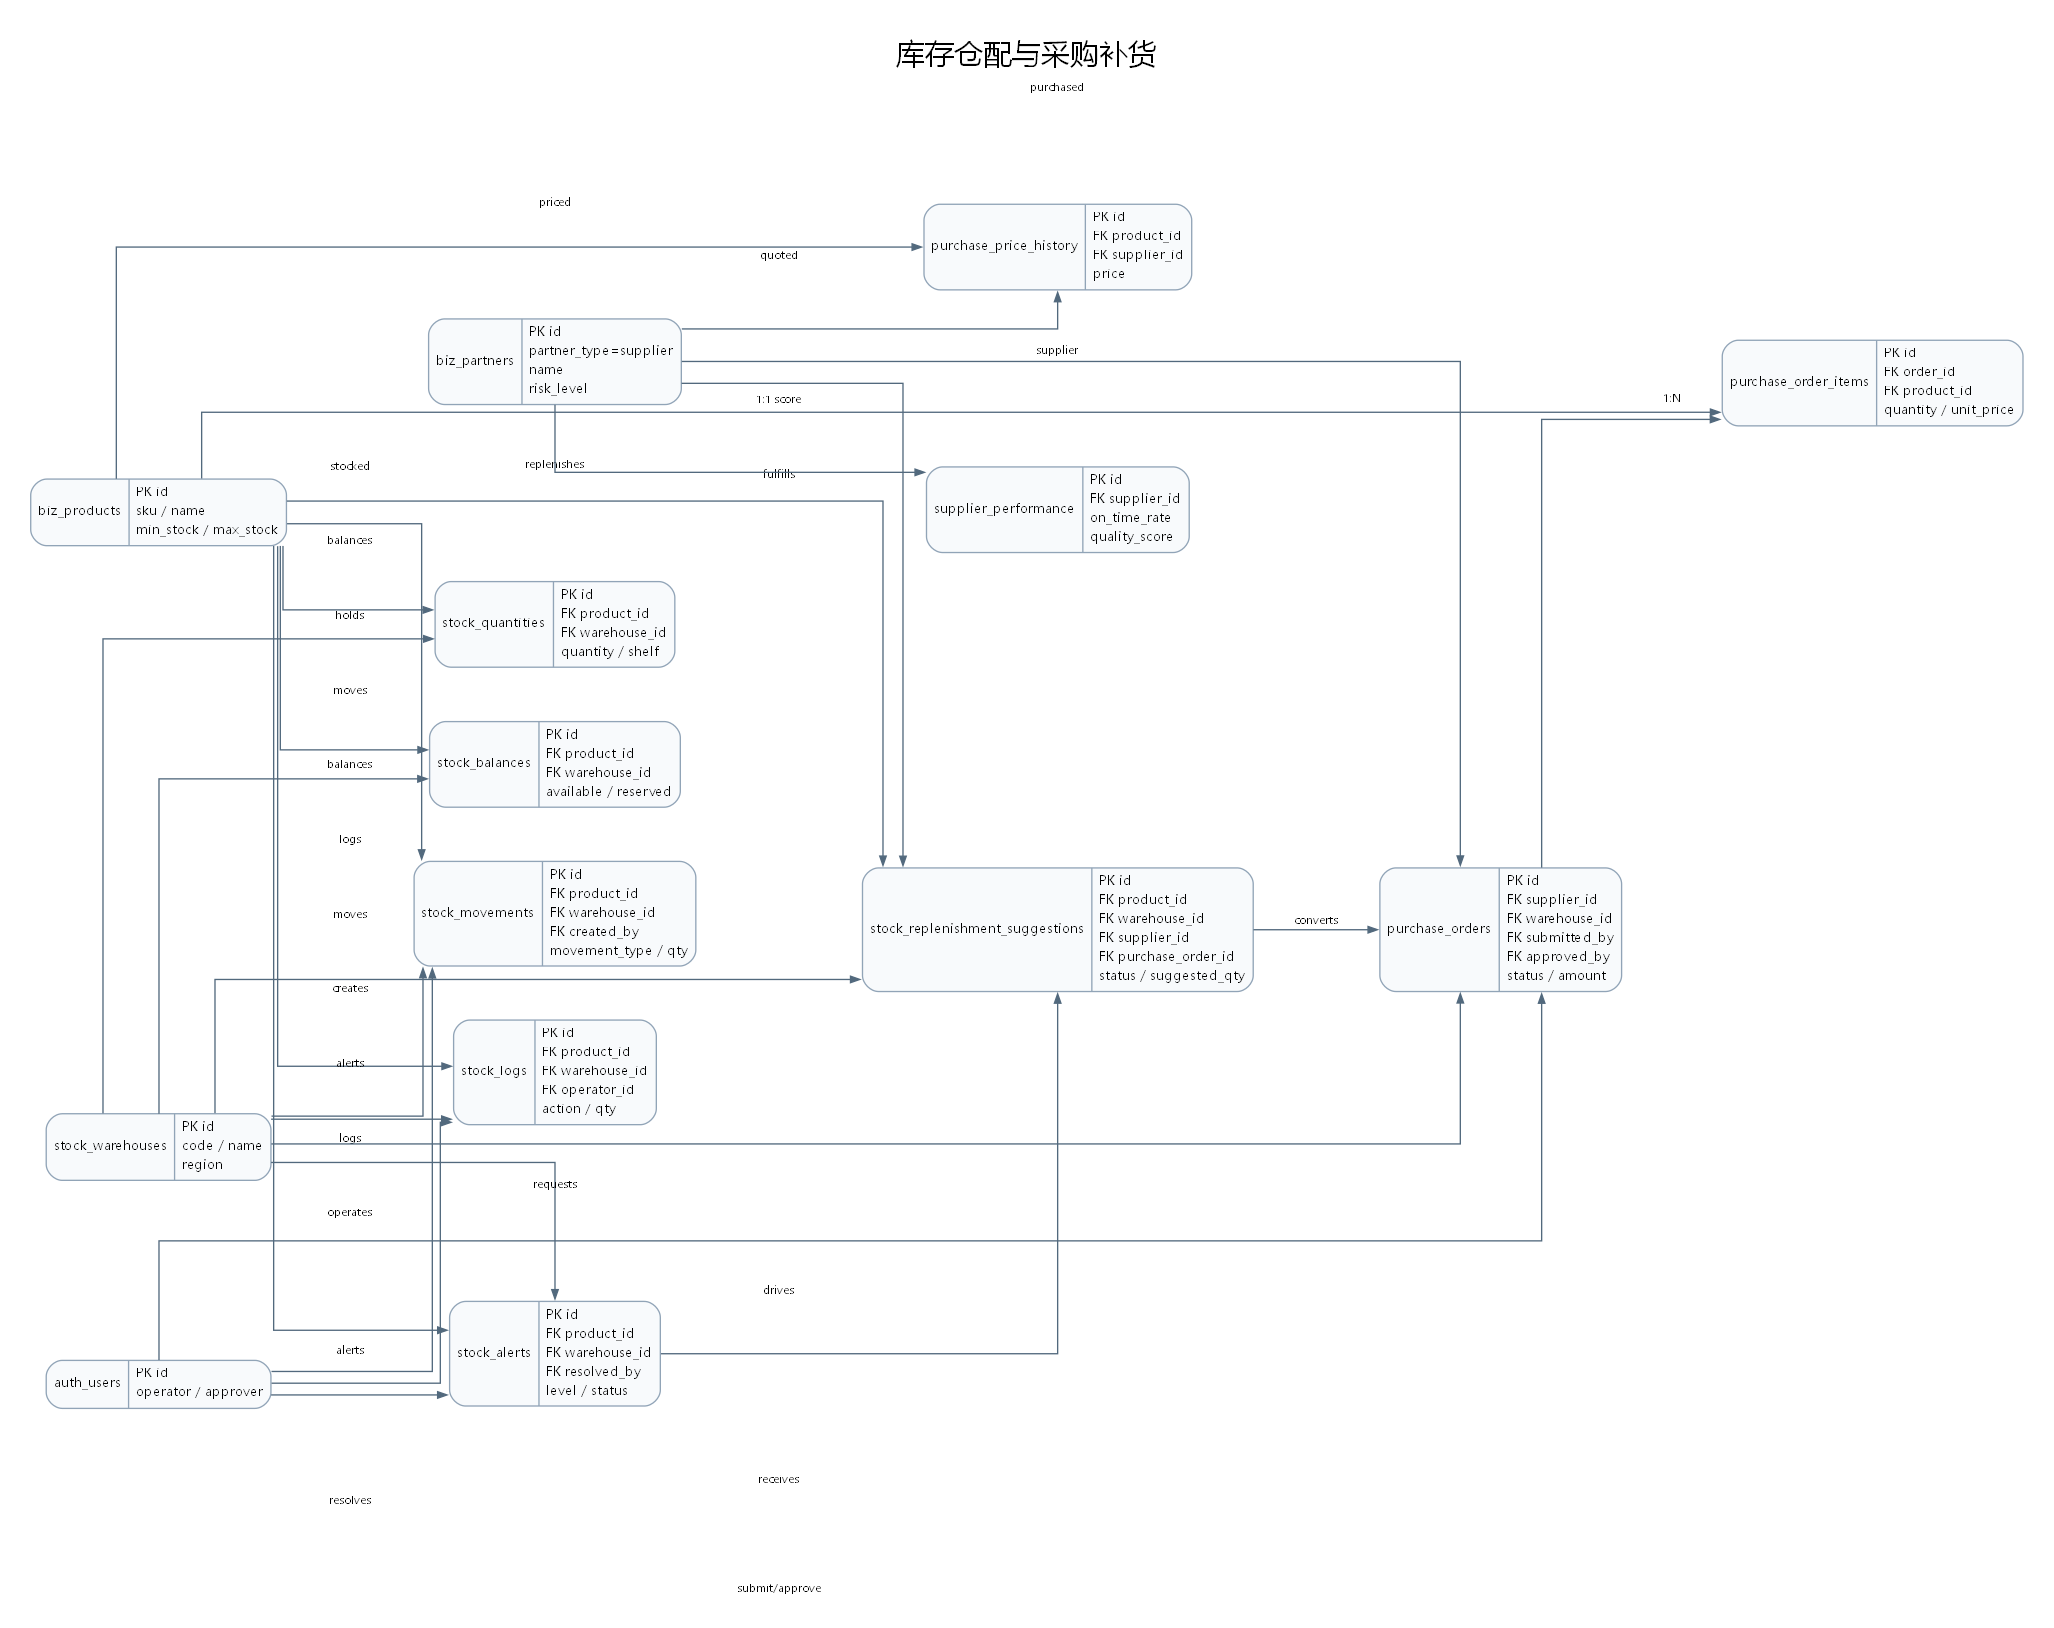
\includegraphics[width=\textwidth,height=0.66\textheight,keepaspectratio]{images/final/er-inventory-procurement.png}
  \caption{库存仓配与采购补货 ER}
\end{figure}
该图覆盖仓库、库存数量、库存余额、库存流水、库存预警、补货建议、采购订单、采购明细、供应商报价和供应商绩效。它解释了从低库存识别到补货建议、采购审批、收货入库、供应商评分的闭环。

这张分域图用于弥补全局 ER 图信息密度过高的问题。全局图负责展示系统全貌，分域图负责在课程讲解时逐个解释表、外键和业务闭环。
\clearpage
\section{销售履约、财务应收与盘点 ER}
\begin{figure}[H]
  \centering
  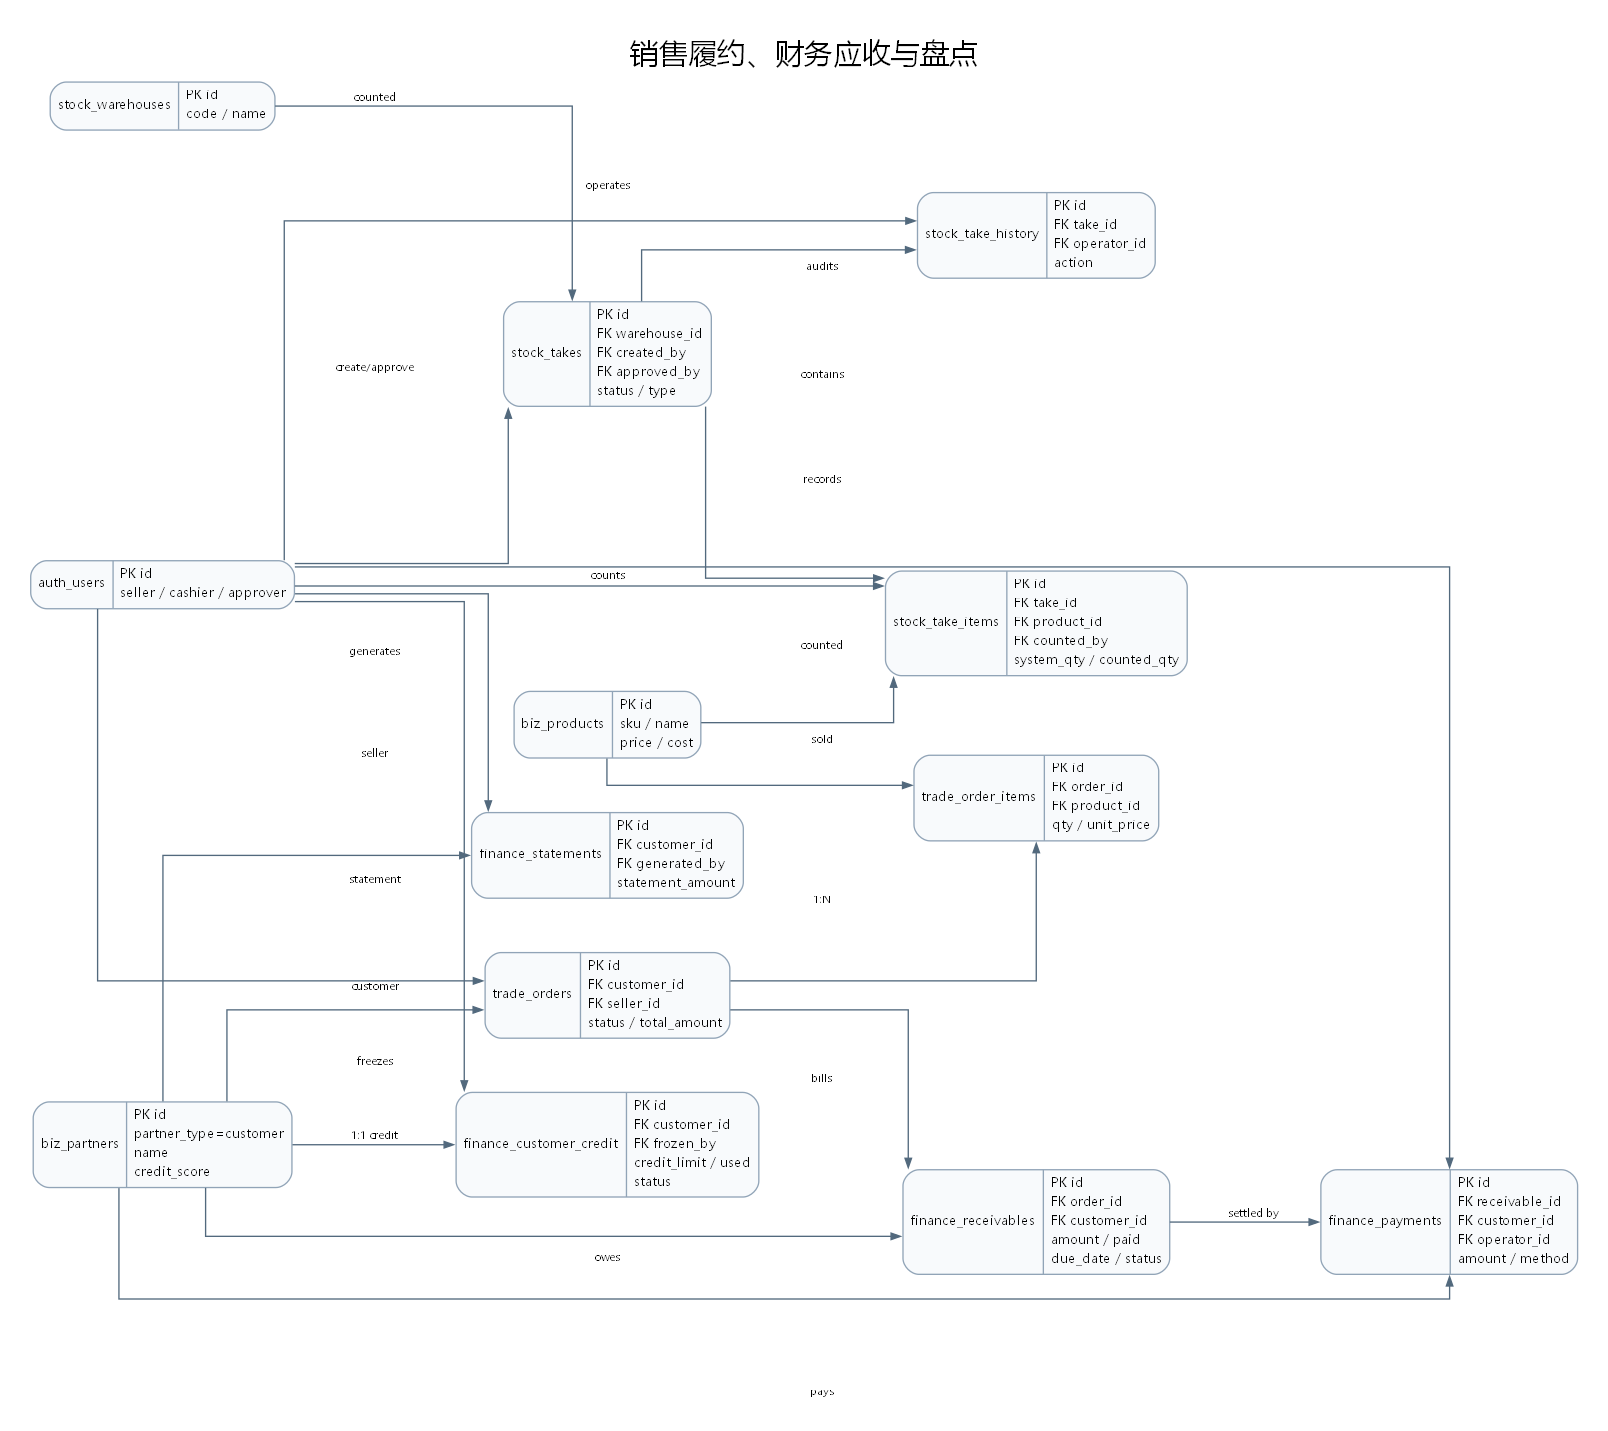
\includegraphics[width=\textwidth,height=0.66\textheight,keepaspectratio]{images/final/er-sales-finance-stocktake.png}
  \caption{销售履约、财务应收与盘点 ER}
\end{figure}
该图覆盖销售订单、销售明细、客户信用、应收、收款、对账单、盘点单、盘点明细和盘点历史。它解释了销售发货后如何形成应收，收款如何核销账龄，盘点差异如何回写库存并进入审计。

这张分域图用于弥补全局 ER 图信息密度过高的问题。全局图负责展示系统全貌，分域图负责在课程讲解时逐个解释表、外键和业务闭环。
\clearpage
\section{工作流、协作、报表与 AI ER}
\begin{figure}[H]
  \centering
  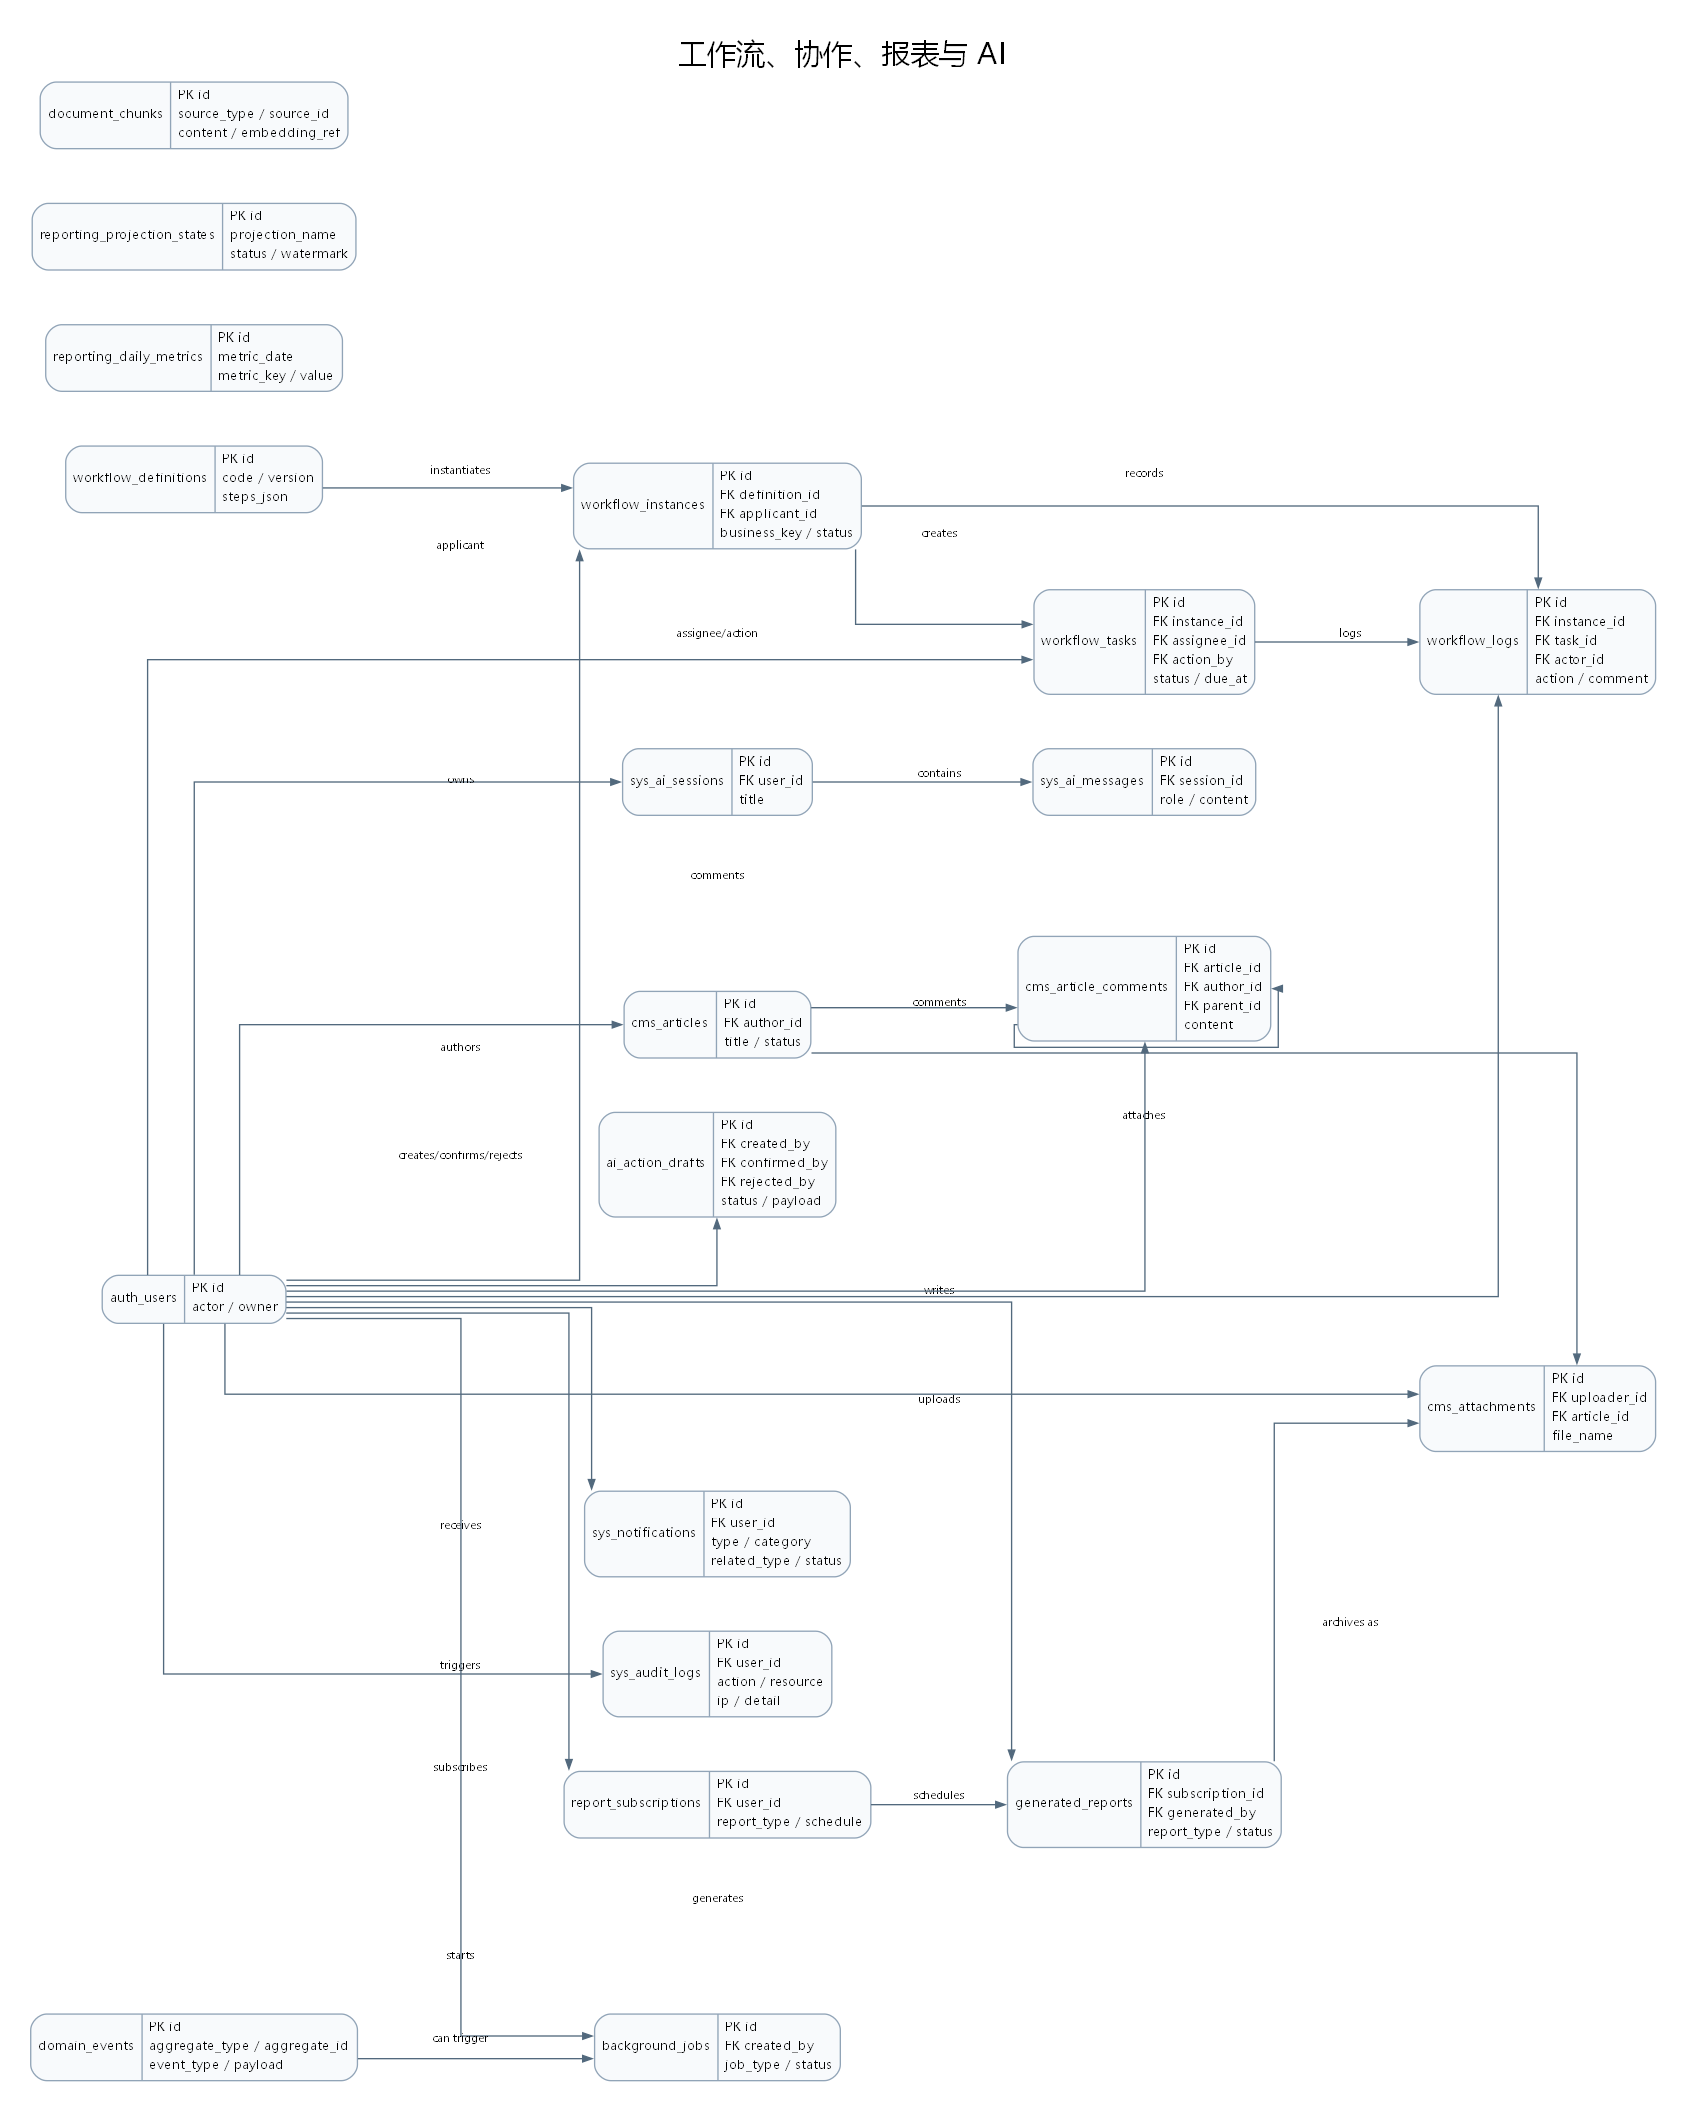
\includegraphics[width=\textwidth,height=0.66\textheight,keepaspectratio]{images/final/er-workflow-collaboration-ai.png}
  \caption{工作流、协作、报表与 AI ER}
\end{figure}
该图覆盖流程定义、流程实例、流程任务、流程日志、通知、公告、评论、附件、报表订阅、生成报表、AI 会话、AI 消息、行动草稿、文档分块、后台任务和领域事件。它解释了系统如何把业务动作变成任务、消息、报表、AI 建议和审计证据。

这张分域图用于弥补全局 ER 图信息密度过高的问题。全局图负责展示系统全貌，分域图负责在课程讲解时逐个解释表、外键和业务闭环。
\clearpage
\section{公共入口页面}
本轮严格遵守约束：首页、登录页、注册页和注册协议页不修改。报告只展示它们在系统流程中的位置，并使用暗色主题截图作为交付材料。
\begin{figure}[H]
  \centering
  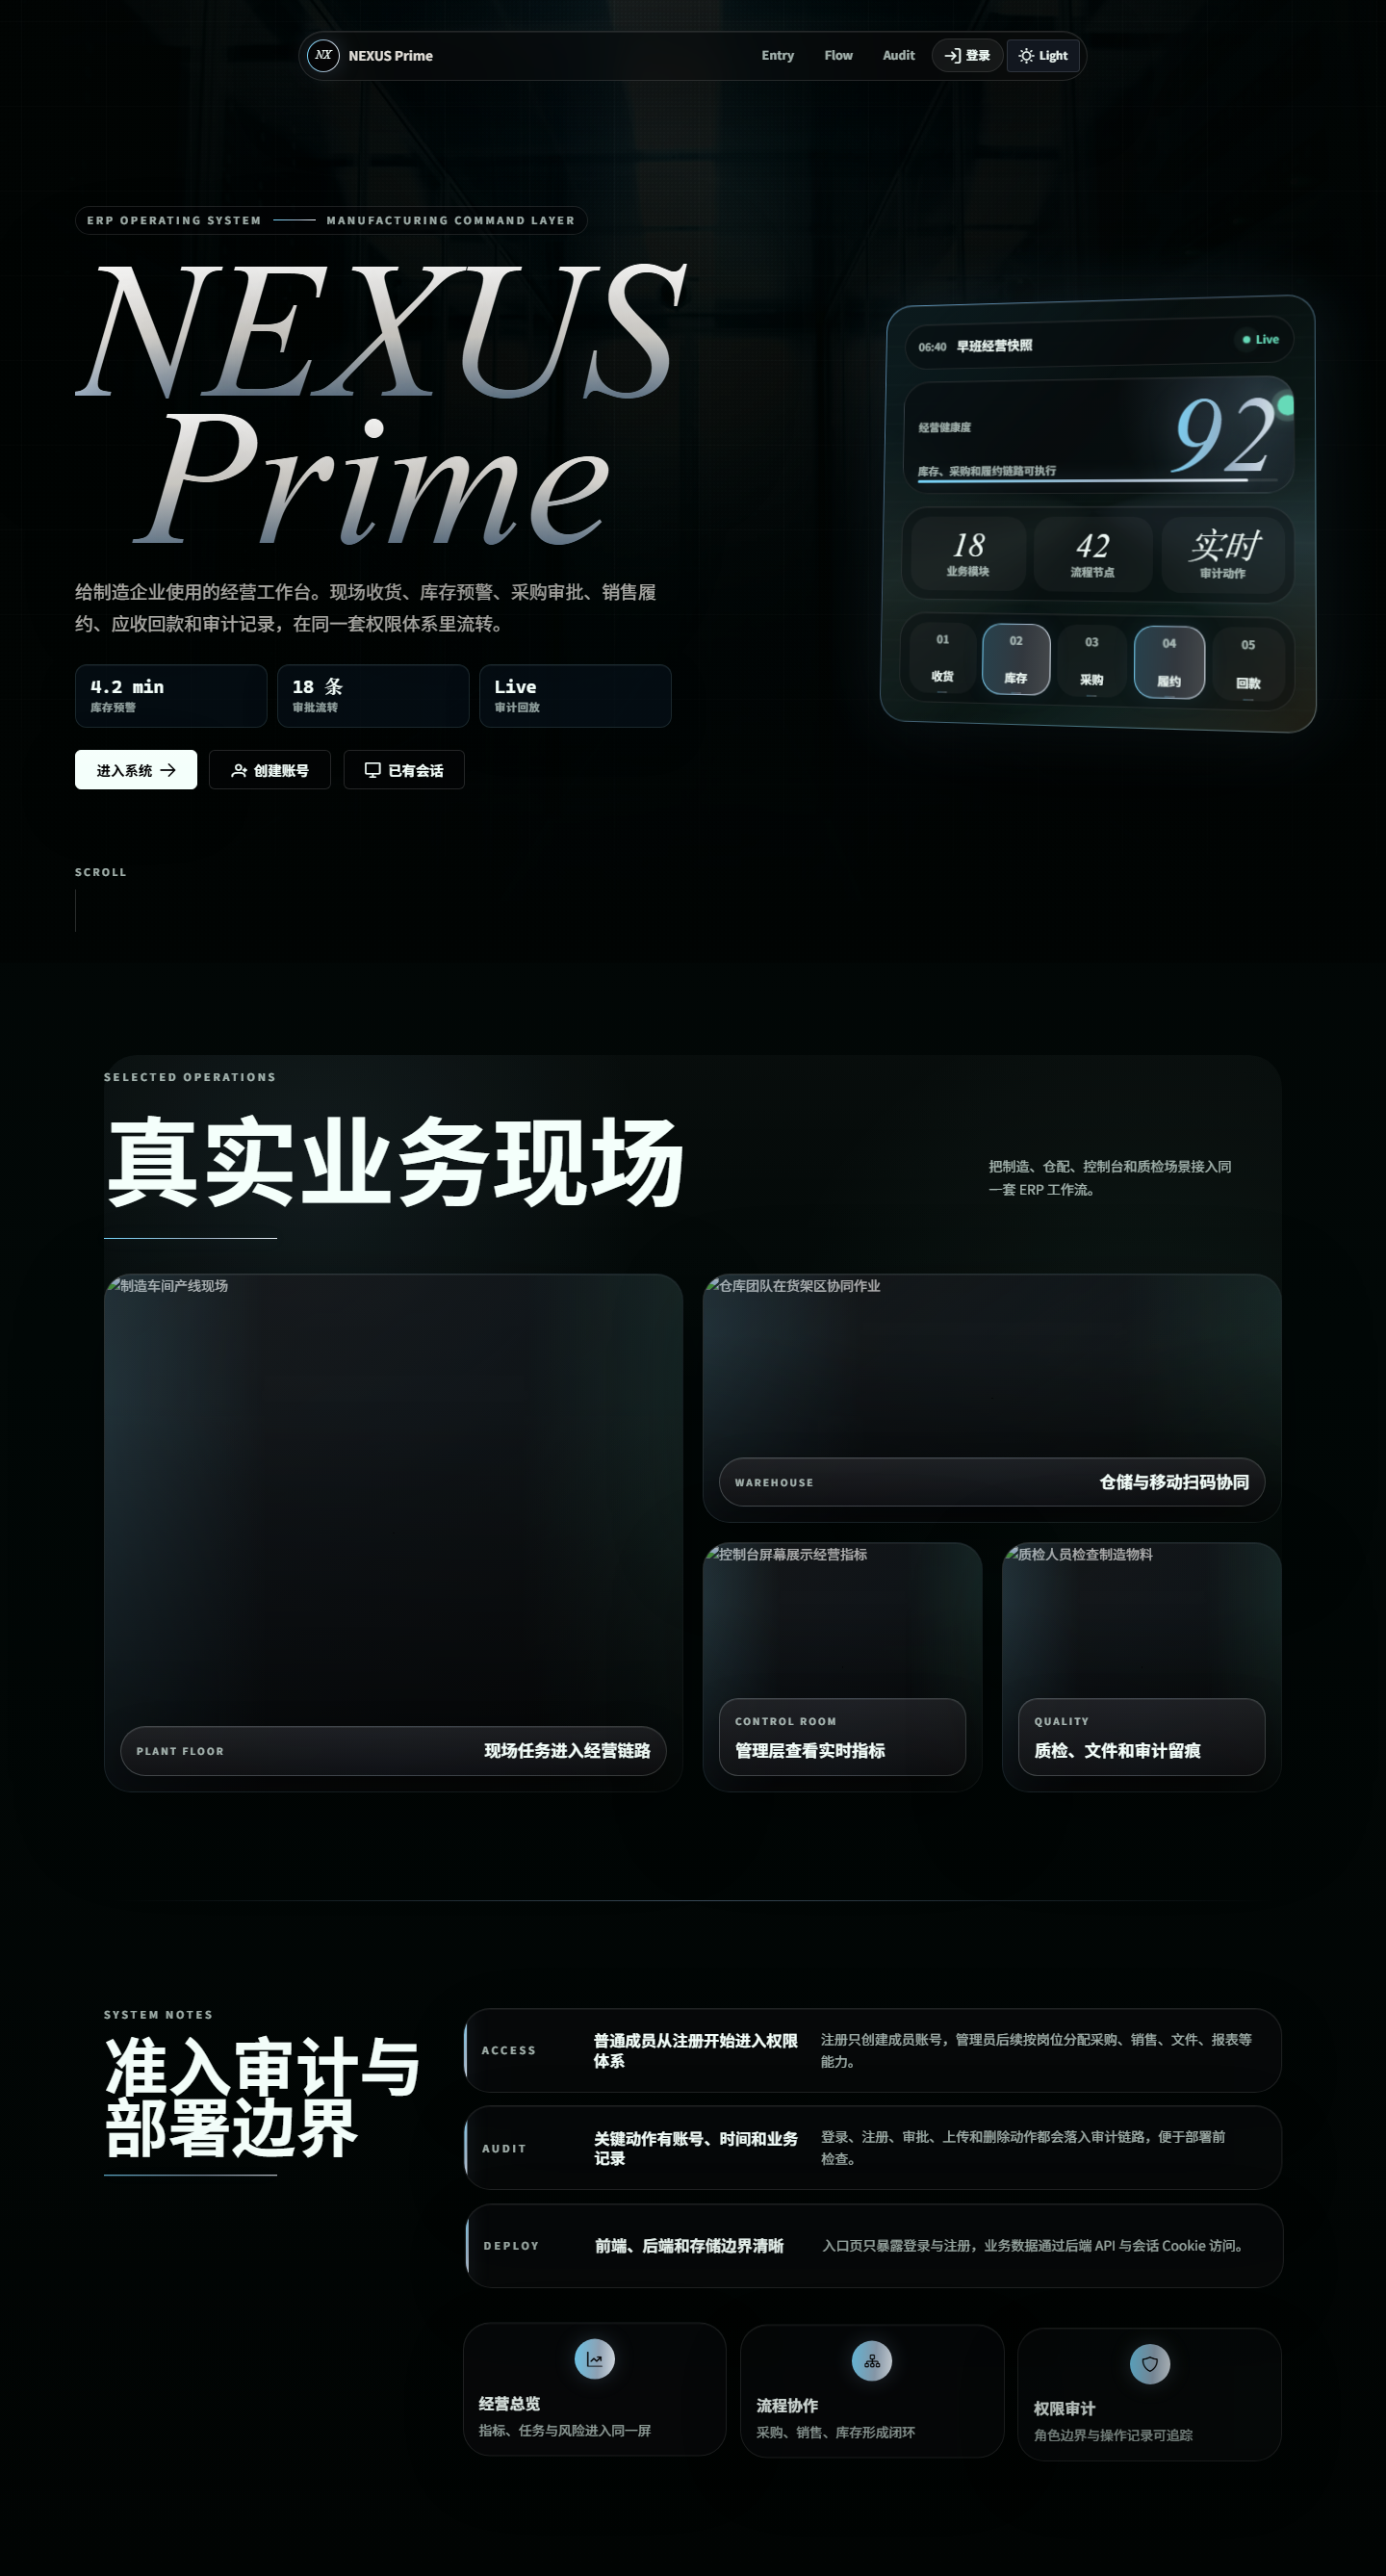
\includegraphics[width=\textwidth,height=0.205\textheight,keepaspectratio]{images/final/entry-dark.png}
  \caption{首页入口，暗色主题截图，源码未修改}
\end{figure}
\tightpara{首页保持原样，仅在报告中使用暗色主题截图。它承担品牌入口、产品气质和进入登录流程的第一视觉锚点。}
\begin{figure}[H]
  \centering
  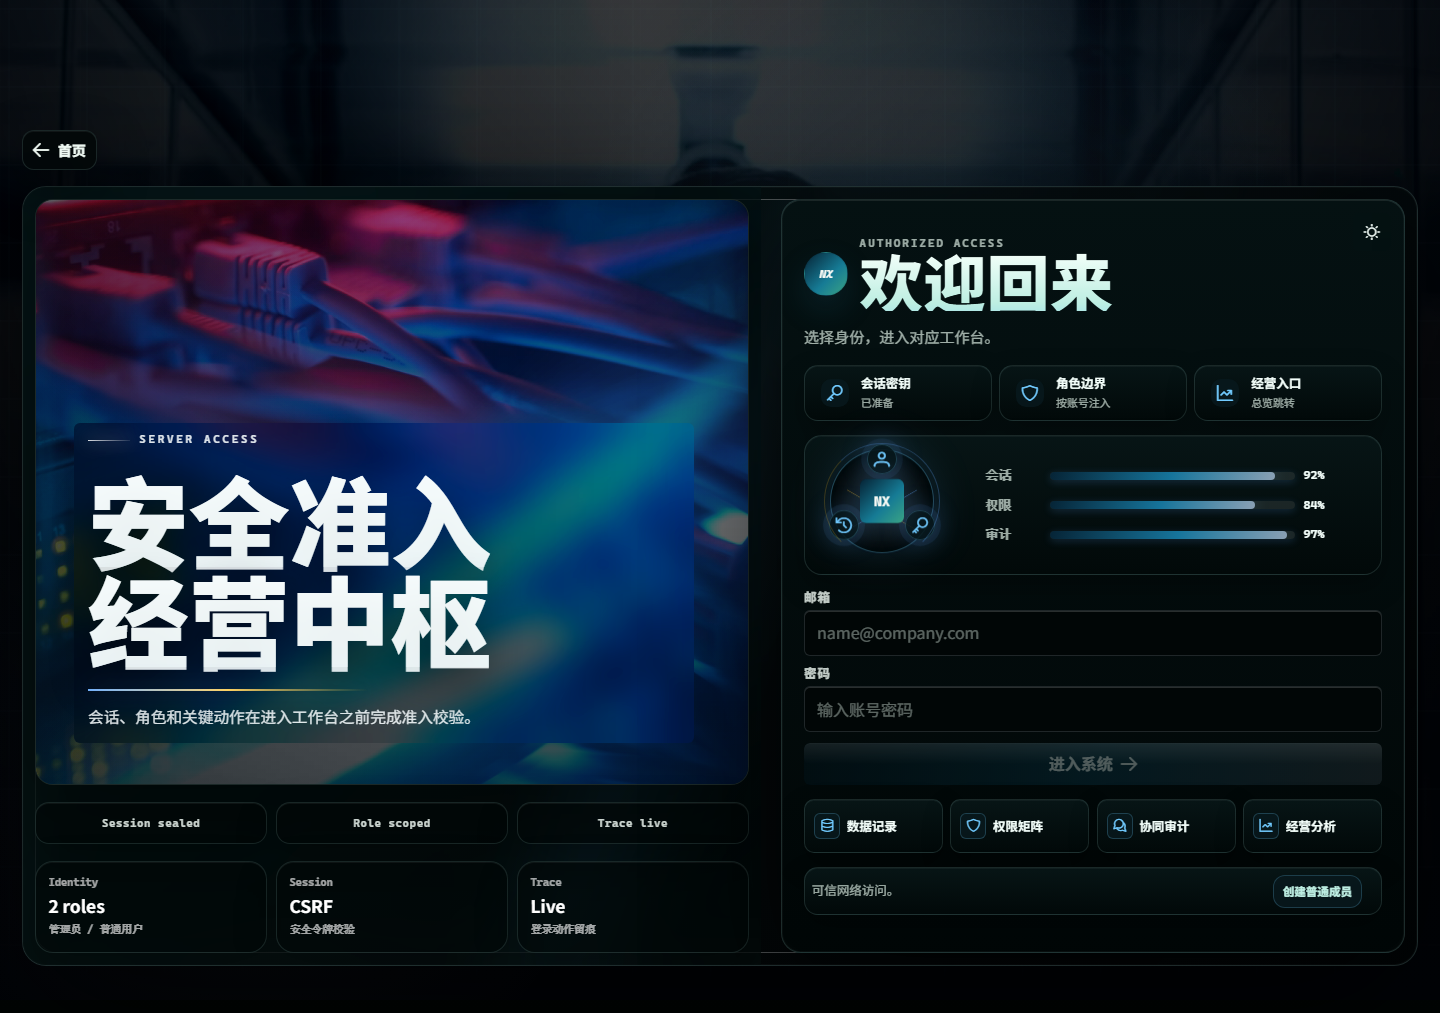
\includegraphics[width=\textwidth,height=0.205\textheight,keepaspectratio]{images/final/login-dark.png}
  \caption{登录页，暗色主题截图，源码未修改}
\end{figure}
\tightpara{登录页保持原样，仅在报告中使用暗色主题截图。它承担账号密码登录、注册切换、会话建立和 CSRF 初始化。}
\begin{figure}[H]
  \centering
  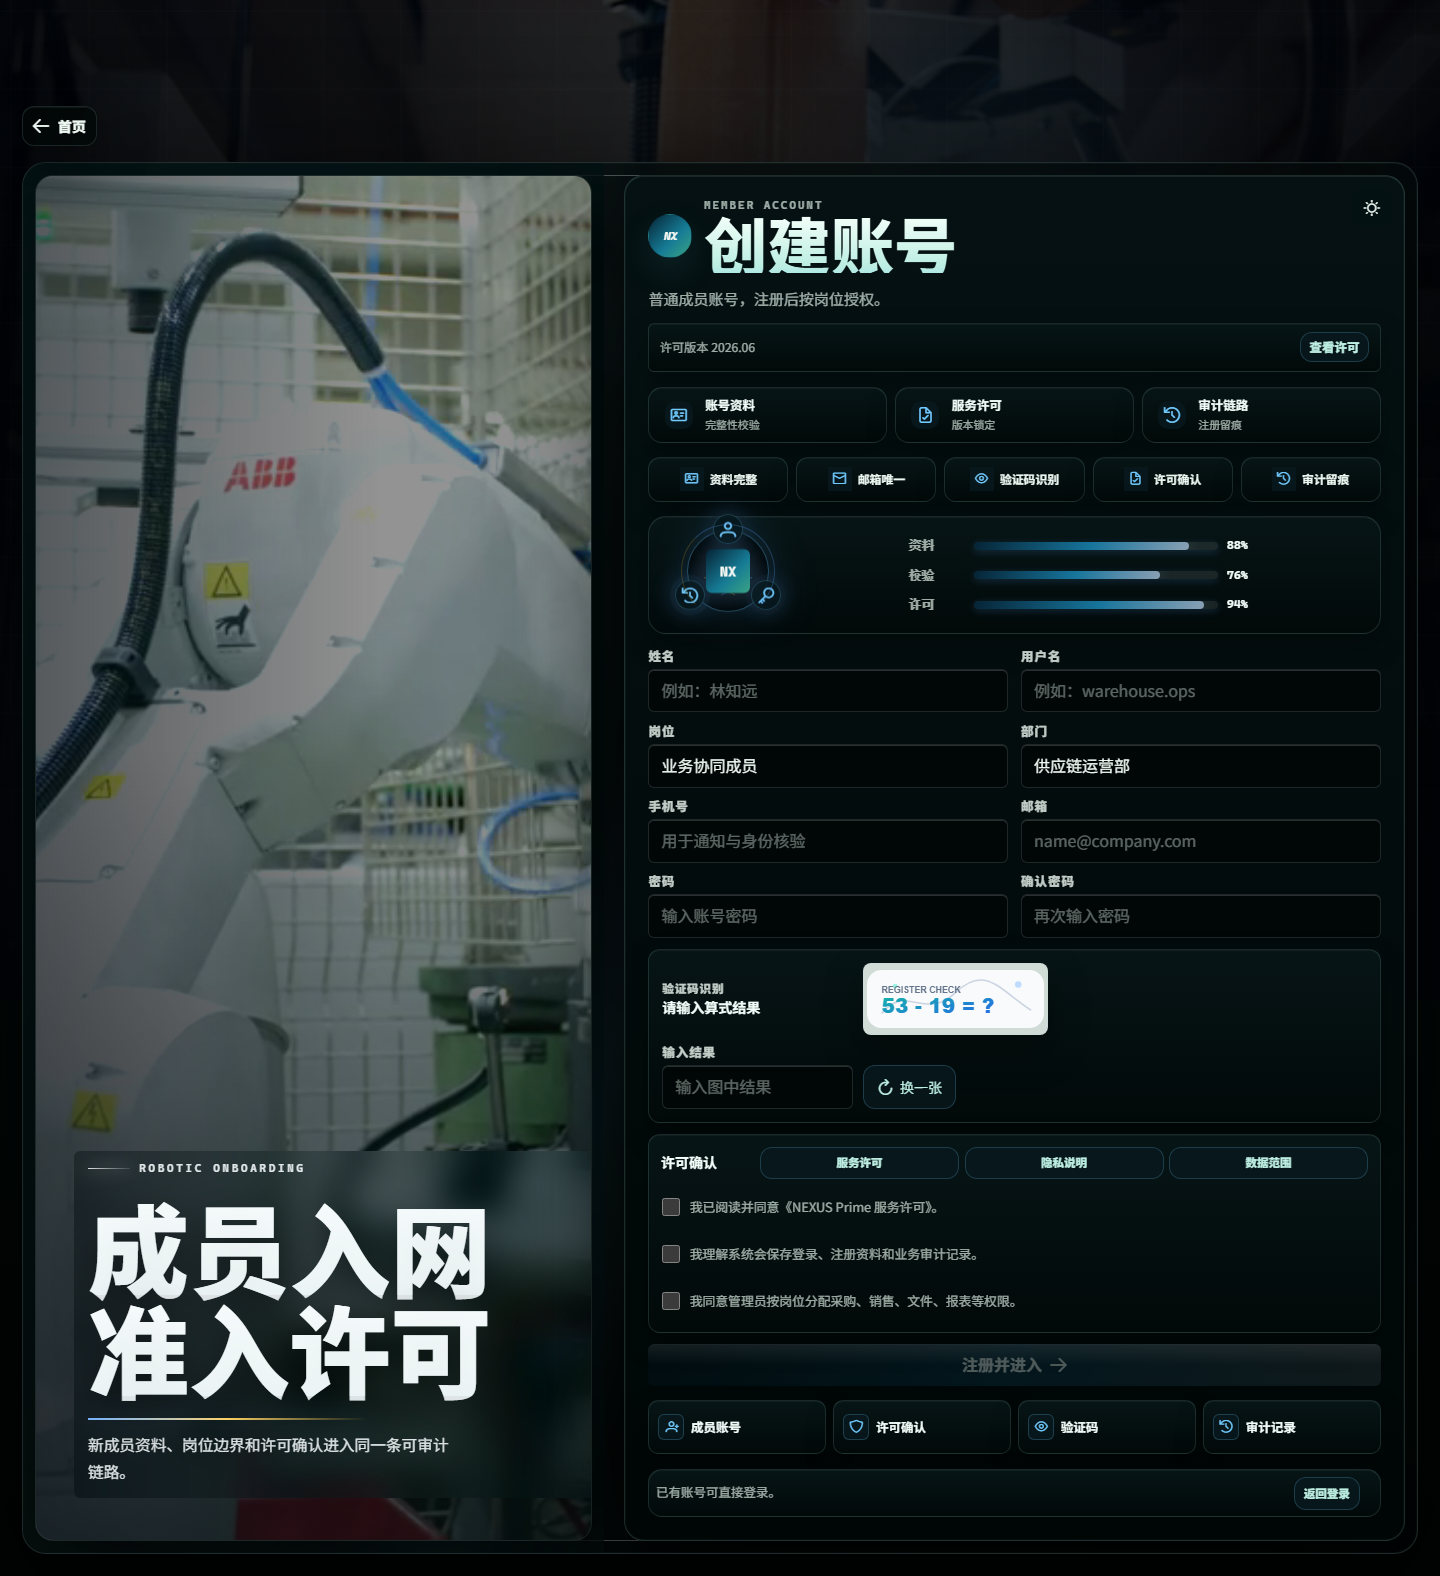
\includegraphics[width=\textwidth,height=0.205\textheight,keepaspectratio]{images/final/register-dark.png}
  \caption{注册页，暗色主题截图，源码未修改}
\end{figure}
\tightpara{注册页保持原样，仅在报告中使用暗色主题截图。它承担普通用户准入、资料填写、协议确认和验证码校验。}
\begin{figure}[H]
  \centering
  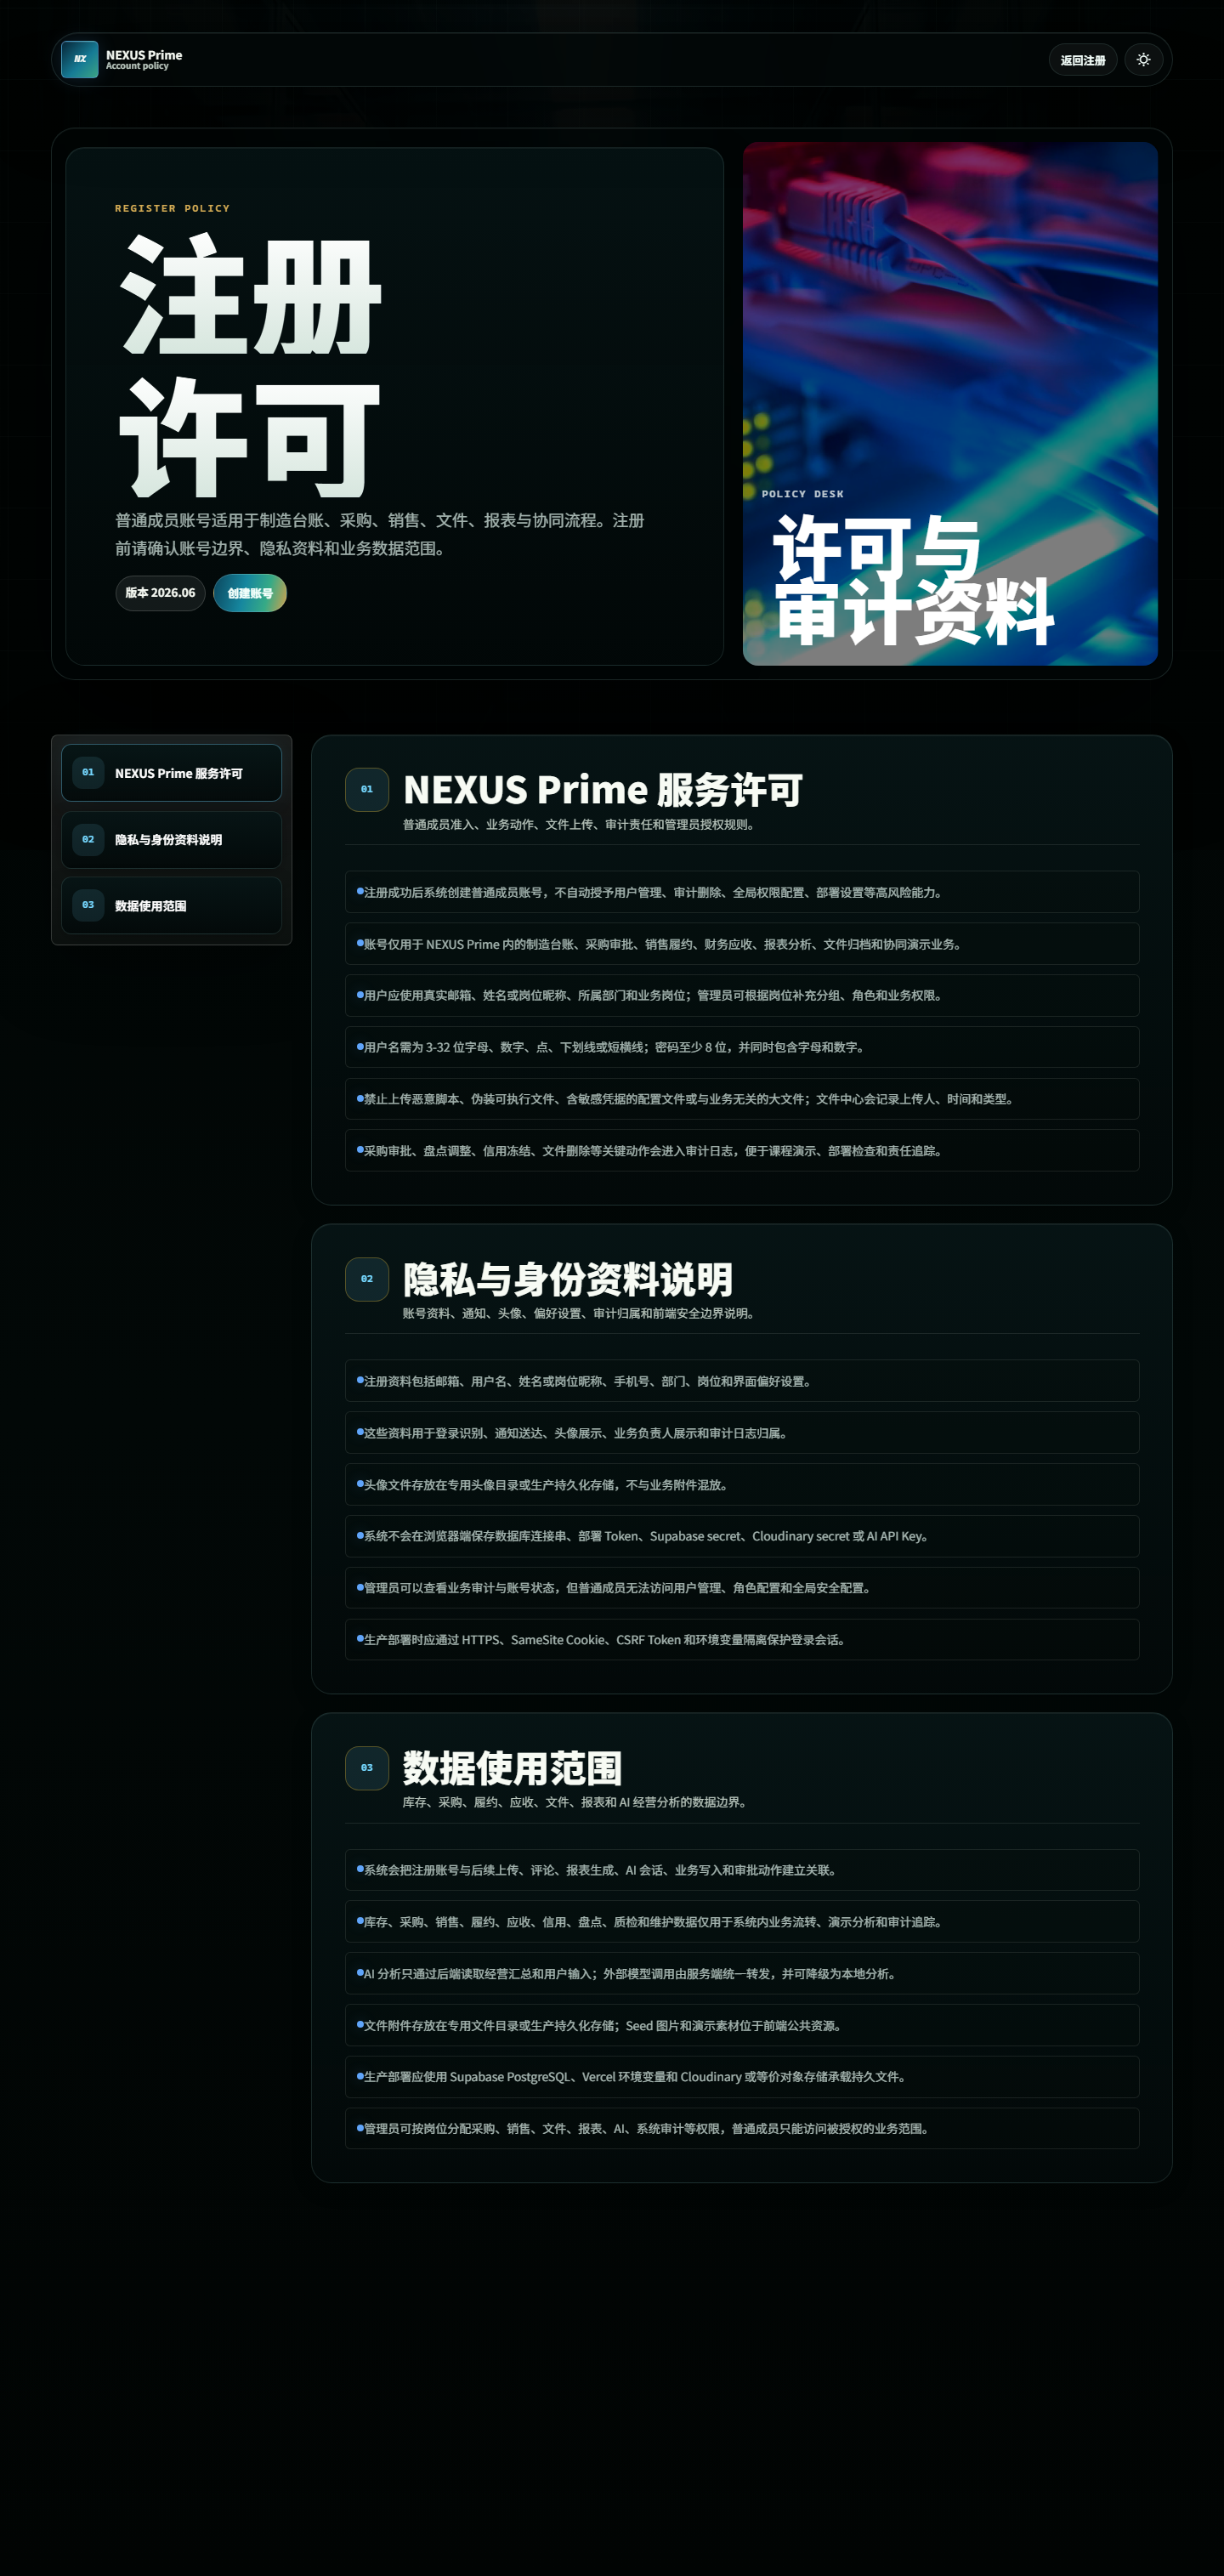
\includegraphics[width=\textwidth,height=0.205\textheight,keepaspectratio]{images/final/register-policy-dark.png}
  \caption{注册协议页，暗色主题截图，源码未修改}
\end{figure}
\tightpara{注册协议页保持原样，仅在报告中使用暗色主题截图。它承担注册规则、隐私说明和用户准入边界说明。}

\clearpage
\section{全部业务页面截图和功能说明}
以下章节从登录后运营首页开始，逐页说明所有业务页面。业务页按顺序使用深色驾驶舱和亮色系统交替截图，既展示主题能力，也展示统一布局在不同背景下的稳定性。每个页面都列出路由、截图、定位、主要功能、数据来源、接口范围、代码关联和升级效果。
\begin{longtable}{p{0.06\textwidth}p{0.2\textwidth}p{0.31\textwidth}p{0.14\textwidth}p{0.19\textwidth}}
\toprule
序号 & 页面 & 路由 & 主题 & 业务域 \\
\midrule
\endhead
1 & 运营控制塔 & \code{/app/overview} & 深色驾驶舱 & 制造指挥中心 \\
2 & 经营指标中心 & \code{/app/metrics} & 亮色系统 & 经营指标 \\
3 & 任务异常中心 & \code{/app/tasks} & 深色驾驶舱 & 待办 \\
4 & 物料库存图谱 & \code{/app/inventory/products} & 亮色系统 & 商品 \\
5 & 仓配流向图 & \code{/app/inventory/stock} & 深色驾驶舱 & 仓库 \\
6 & 采购补货建议 & \code{/app/inventory/replenishment} & 亮色系统 & 补货建议 \\
7 & 客户窗口与发货调度台 & \code{/app/sales/orders} & 深色驾驶舱 & 销售订单 \\
8 & 采购协同控制台 & \code{/app/procurement/orders} & 亮色系统 & 采购订单 \\
9 & 供应商协同 & \code{/app/suppliers/performance} & 深色驾驶舱 & 供应商绩效 \\
10 & 仓配调度中心 & \code{/app/dispatch} & 亮色系统 & 仓库 \\
11 & 数据质量中心 & \code{/app/data-quality} & 深色驾驶舱 & 商品 \\
12 & 质量检验中心 & \code{/app/quality} & 亮色系统 & 质量任务 \\
13 & 客户经营中心 & \code{/app/customers} & 深色驾驶舱 & 客户伙伴 \\
14 & 产能计划中心 & \code{/app/capacity} & 亮色系统 & 产能计划 \\
15 & 设备维护中心 & \code{/app/maintenance} & 深色驾驶舱 & 设备 \\
16 & 合同回款中心 & \code{/app/contracts} & 亮色系统 & 合同 \\
17 & 售后服务中心 & \code{/app/service} & 深色驾驶舱 & 客户 \\
18 & 规则引擎中心 & \code{/app/rules} & 亮色系统 & 规则 \\
19 & 集成监控中心 & \code{/app/integrations} & 深色驾驶舱 & 后台任务 \\
20 & 预算成本中心 & \code{/app/budget} & 亮色系统 & 采购 \\
21 & 移动扫码终端 & \code{/app/mobile-terminal} & 深色驾驶舱 & 移动任务 \\
22 & 账龄风险墙 & \code{/app/finance/receivables} & 亮色系统 & 应收 \\
23 & 客户信用中心 & \code{/app/finance/credits} & 深色驾驶舱 & 客户信用 \\
24 & 库存盘点中心 & \code{/app/stocktakes} & 亮色系统 & 盘点单 \\
25 & 报表工作室 & \code{/app/reports} & 深色驾驶舱 & 生成报表 \\
26 & 文件资料库 & \code{/app/files} & 亮色系统 & 附件 \\
27 & 公告与知识库 & \code{/app/content/articles} & 深色驾驶舱 & 文章 \\
28 & 系统安全中心 & \code{/app/system/users} & 亮色系统 & 用户 \\
29 & 审计日志 & \code{/app/system/audit} & 深色驾驶舱 & 审计日志 \\
30 & 任务通知中心 & \code{/app/notifications} & 亮色系统 & 系统通知 \\
31 & 经营分析台 & \code{/app/ai} & 深色驾驶舱 & AI 会话 \\
32 & 个人中心 & \code{/app/profile} & 亮色系统 & 当前用户 \\
33 & 控制中心 & \code{/app/settings} & 深色驾驶舱 & 个人偏好 \\
\bottomrule
\end{longtable}

上表先给出完整页面地图，后续每页再展开截图、功能、数据、接口和代码关联。这样报告从入口、ER、架构到所有业务页面是一条连续链路，而不是零散截图集合。
\clearpage
\subsection{1. 运营控制塔}
\begin{figure}[H]
  \centering
  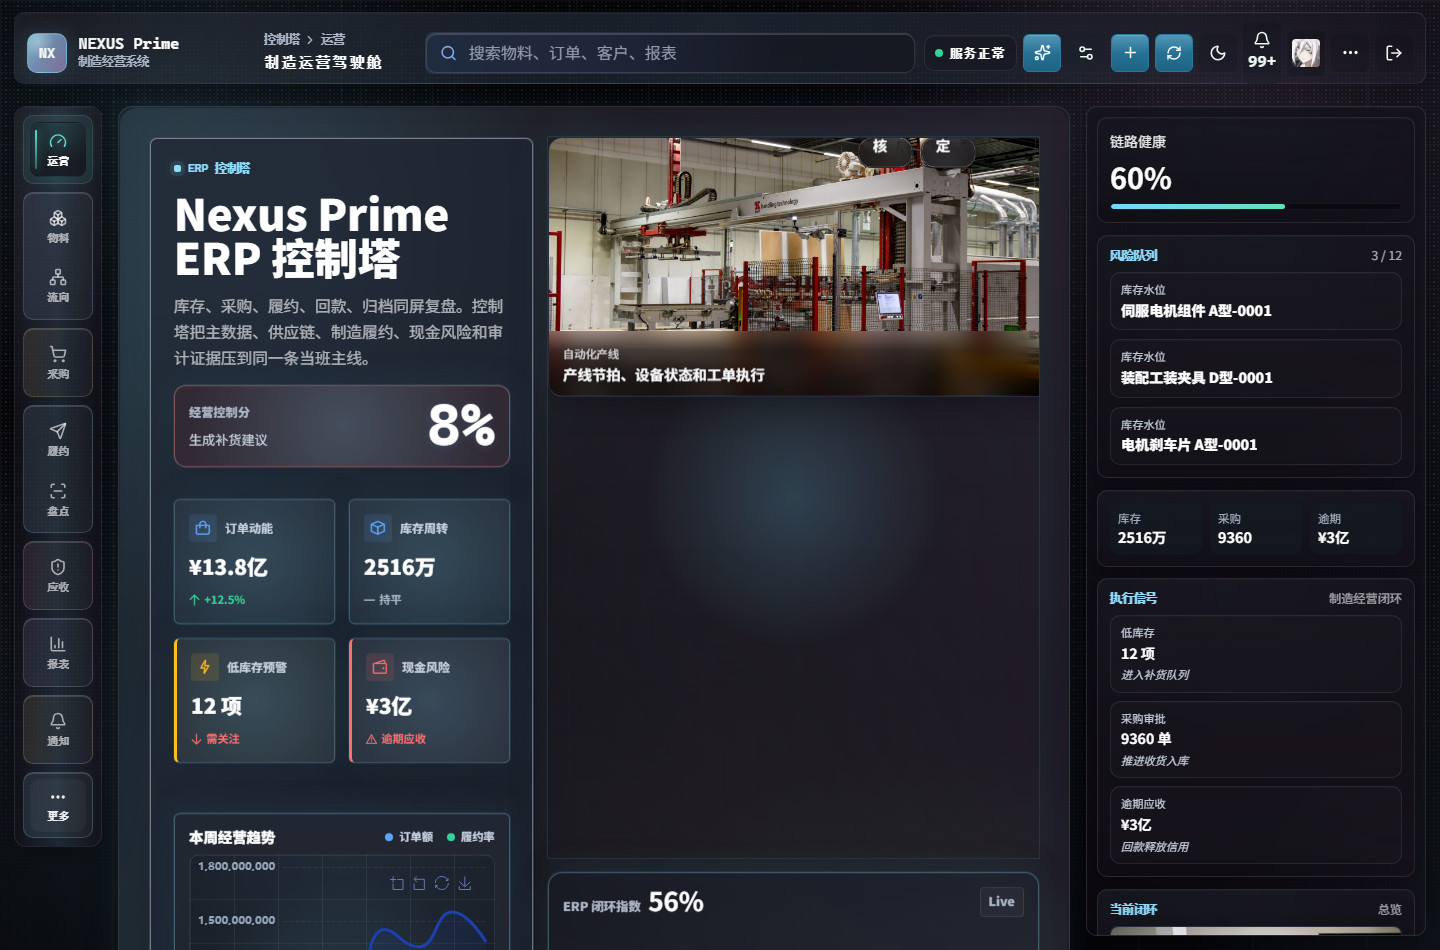
\includegraphics[width=\textwidth,height=0.38\textheight,keepaspectratio]{images/final/pages/desktop-dark-cockpit-overview.png}
  \caption{运营控制塔桌面截图，深色驾驶舱}
\end{figure}
\begin{tabularx}{\textwidth}{>{\bfseries}p{0.16\textwidth}X>{\bfseries}p{0.16\textwidth}X}
\toprule
路由 & \code{/app/overview} & 展示主题 & 深色驾驶舱 \\
主要数据 & 制造指挥中心、待办任务、异常队列、库存和财务摘要。 & 主要接口 & \code{manufacturing/command-center, operations/todo, operations/exceptions} \\
代码关联 & \multicolumn{3}{p{0.7\textwidth}}{\small AppShell + command-center.page.ts + operations APIs} \\
\bottomrule
\end{tabularx}
\vspace{0.5em}
\tightpara{\textbf{页面定位：}作为登录后的总览页，把库存、采购、销售、应收、异常任务和经营风险合并为一个运营控制塔。}
\tightpara{\textbf{升级效果：}运营域强调经营指标、任务异常、产能和设备状态，目标是把管理者每天先看的信息放在同一层。页面不再用零散跳转块，而是以态势图、风险队列和执行列表组织。本页按照“真实图和关键图表在上、交互报表在中、表单和分页操作台在下”的规则整理，减少无意义跳转方框，让业务动作和数据对象保持同一条线。}
\begin{multicols}{2}
\textbf{主要功能}
\begin{itemize}
  \item 查看经营控制分和核心 KPI
  \item 进入库存、采购、销售、财务等业务闭环
  \item 查看当班待办、风险提示和趋势图
\end{itemize}
\columnbreak
\textbf{验收关注}
\begin{itemize}
  \item 上方区域优先展示真实图、态势图和关键指标，不再堆叠重复入口。
  \item 下方操作台承担搜索、分页、创建、编辑、删除、导出和领域动作。
  \item 页面跳转由 Dock、顶部搜索和资源操作台统一管理，避免随机跳转。
\end{itemize}
\end{multicols}
\clearpage
\subsection{2. 经营指标中心}
\begin{figure}[H]
  \centering
  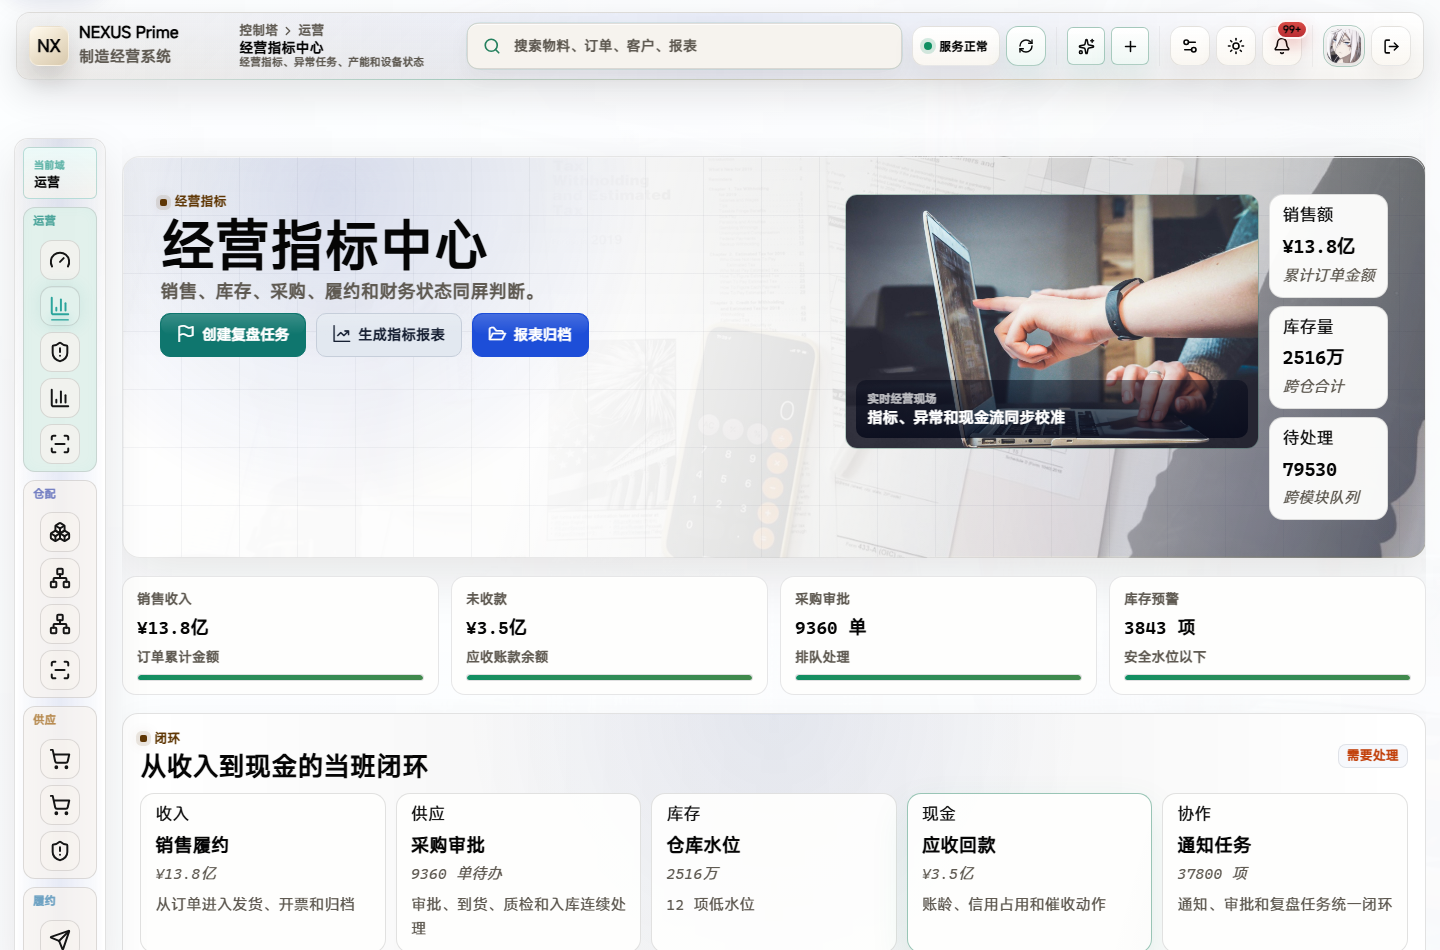
\includegraphics[width=\textwidth,height=0.38\textheight,keepaspectratio]{images/final/pages/desktop-light-luxury-metrics.png}
  \caption{经营指标中心桌面截图，亮色系统}
\end{figure}
\begin{tabularx}{\textwidth}{>{\bfseries}p{0.16\textwidth}X>{\bfseries}p{0.16\textwidth}X}
\toprule
路由 & \code{/app/metrics} & 展示主题 & 亮色系统 \\
主要数据 & 经营指标、库存水位、销售和财务汇总。 & 主要接口 & \code{analytics/executive} \\
代码关联 & \multicolumn{3}{p{0.7\textwidth}}{\small executive-metrics.page.ts + analytics/executive} \\
\bottomrule
\end{tabularx}
\vspace{0.5em}
\tightpara{\textbf{页面定位：}经营指标中心用于展示业务健康度、营收趋势、库存效率和现金流风险。}
\tightpara{\textbf{升级效果：}运营域强调经营指标、任务异常、产能和设备状态，目标是把管理者每天先看的信息放在同一层。页面不再用零散跳转块，而是以态势图、风险队列和执行列表组织。本页按照“真实图和关键图表在上、交互报表在中、表单和分页操作台在下”的规则整理，减少无意义跳转方框，让业务动作和数据对象保持同一条线。}
\begin{multicols}{2}
\textbf{主要功能}
\begin{itemize}
  \item 查看核心经营指标
  \item 对比多维度图表
  \item 识别异常指标并进入相关业务页
\end{itemize}
\columnbreak
\textbf{验收关注}
\begin{itemize}
  \item 上方区域优先展示真实图、态势图和关键指标，不再堆叠重复入口。
  \item 下方操作台承担搜索、分页、创建、编辑、删除、导出和领域动作。
  \item 页面跳转由 Dock、顶部搜索和资源操作台统一管理，避免随机跳转。
\end{itemize}
\end{multicols}
\clearpage
\subsection{3. 任务异常中心}
\begin{figure}[H]
  \centering
  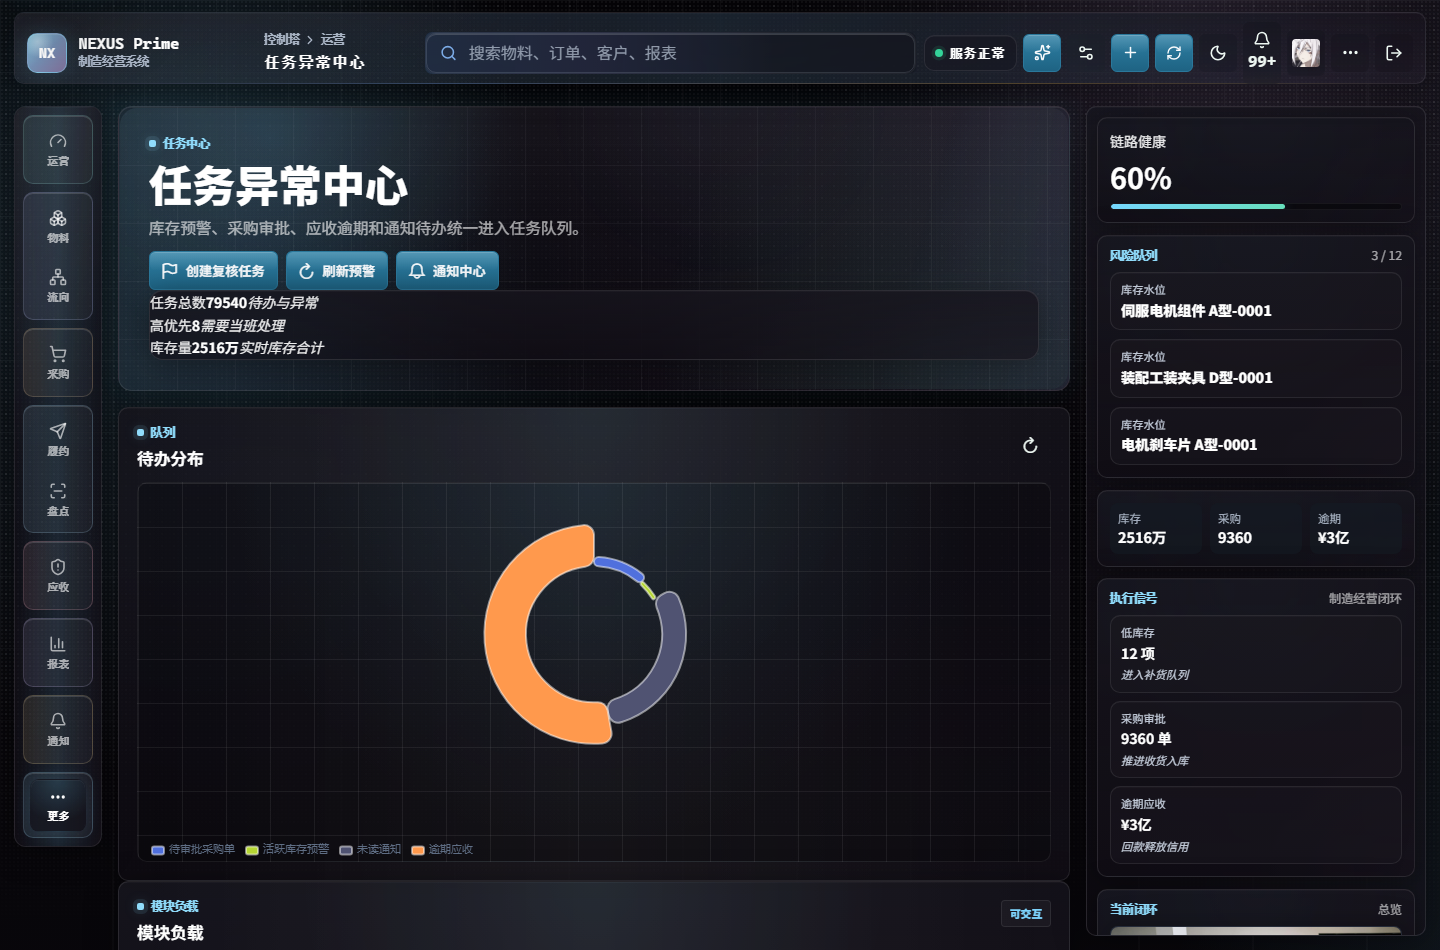
\includegraphics[width=\textwidth,height=0.38\textheight,keepaspectratio]{images/final/pages/desktop-dark-cockpit-tasks.png}
  \caption{任务异常中心桌面截图，深色驾驶舱}
\end{figure}
\begin{tabularx}{\textwidth}{>{\bfseries}p{0.16\textwidth}X>{\bfseries}p{0.16\textwidth}X}
\toprule
路由 & \code{/app/tasks} & 展示主题 & 深色驾驶舱 \\
主要数据 & 待办、异常、流程任务和通知。 & 主要接口 & \code{operations/todo, operations/exceptions, notifications} \\
代码关联 & \multicolumn{3}{p{0.7\textwidth}}{\small operations-tasks.page.ts + operations/todo + notifications} \\
\bottomrule
\end{tabularx}
\vspace{0.5em}
\tightpara{\textbf{页面定位：}任务异常中心把超期、堵点、审批、库存和质量异常集中到统一队列。}
\tightpara{\textbf{升级效果：}运营域强调经营指标、任务异常、产能和设备状态，目标是把管理者每天先看的信息放在同一层。页面不再用零散跳转块，而是以态势图、风险队列和执行列表组织。本页按照“真实图和关键图表在上、交互报表在中、表单和分页操作台在下”的规则整理，减少无意义跳转方框，让业务动作和数据对象保持同一条线。}
\begin{multicols}{2}
\textbf{主要功能}
\begin{itemize}
  \item 查看异常任务
  \item 按状态和优先级识别风险
  \item 从异常跳转到具体业务对象
\end{itemize}
\columnbreak
\textbf{验收关注}
\begin{itemize}
  \item 上方区域优先展示真实图、态势图和关键指标，不再堆叠重复入口。
  \item 下方操作台承担搜索、分页、创建、编辑、删除、导出和领域动作。
  \item 页面跳转由 Dock、顶部搜索和资源操作台统一管理，避免随机跳转。
\end{itemize}
\end{multicols}
\clearpage
\subsection{4. 物料库存图谱}
\begin{figure}[H]
  \centering
  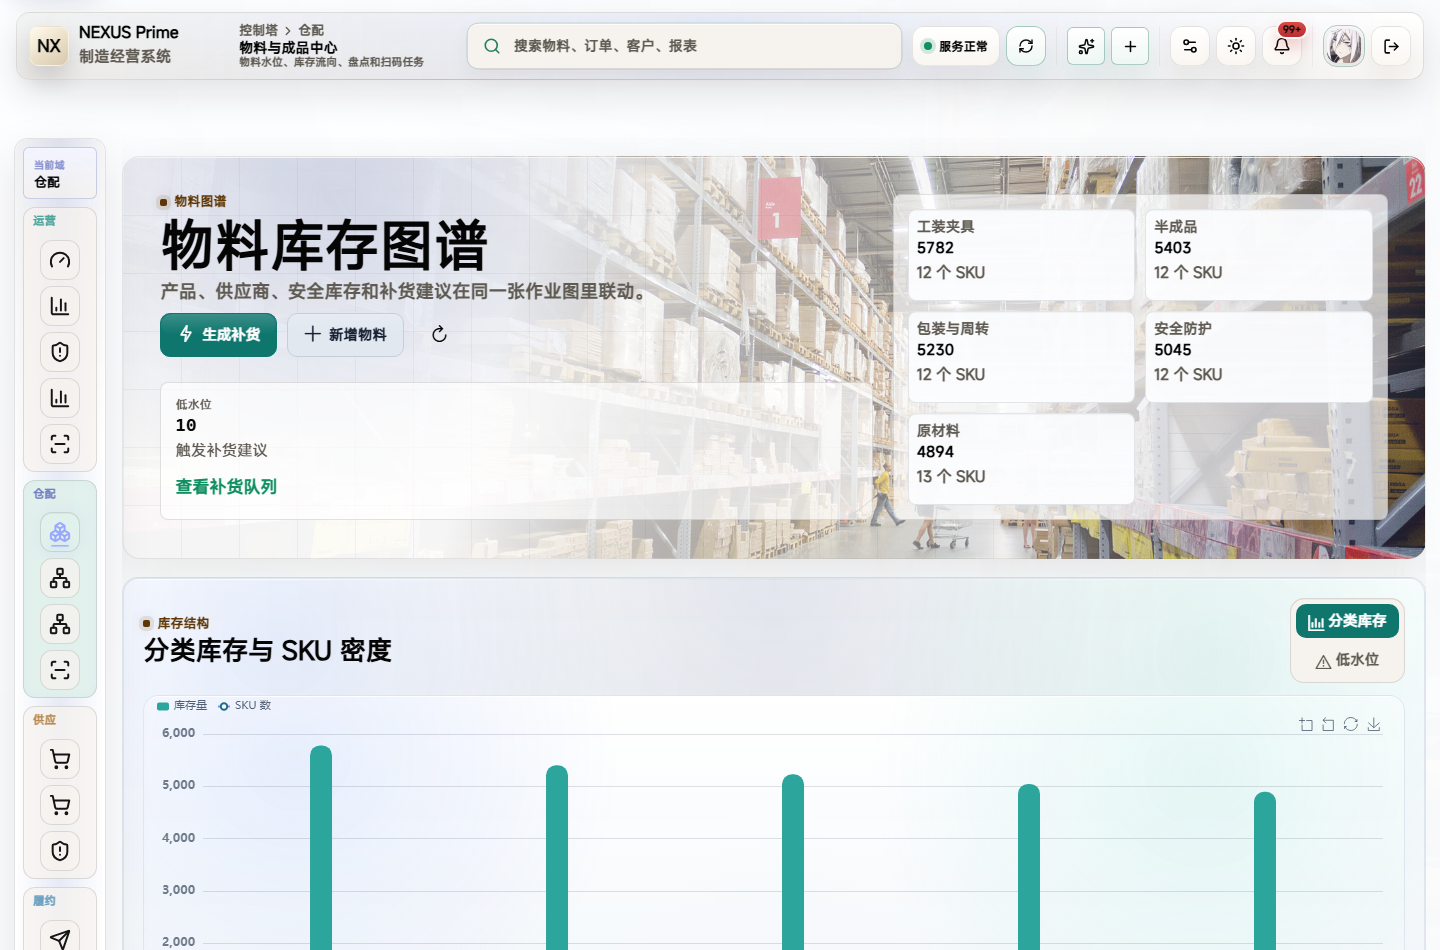
\includegraphics[width=\textwidth,height=0.38\textheight,keepaspectratio]{images/final/pages/desktop-light-luxury-inventory-products.png}
  \caption{物料库存图谱桌面截图，亮色系统}
\end{figure}
\begin{tabularx}{\textwidth}{>{\bfseries}p{0.16\textwidth}X>{\bfseries}p{0.16\textwidth}X}
\toprule
路由 & \code{/app/inventory/products} & 展示主题 & 亮色系统 \\
主要数据 & 商品、分类、供应商、标签和库存数量。 & 主要接口 & \code{products, categories, partners, inventory} \\
代码关联 & \multicolumn{3}{p{0.7\textwidth}}{\small ResourceWorkbench + products 资源配置 + materials.page.ts} \\
\bottomrule
\end{tabularx}
\vspace{0.5em}
\tightpara{\textbf{页面定位：}物料库存图谱管理产品主数据、分类、供应商和库存关联。}
\tightpara{\textbf{升级效果：}仓配域围绕物料、库存、仓库、库位、扫码和盘点。上方看库存真实场景和流向，中间看交互报表，下方用统一操作台处理库存变动、分页和记录检查。本页按照“真实图和关键图表在上、交互报表在中、表单和分页操作台在下”的规则整理，减少无意义跳转方框，让业务动作和数据对象保持同一条线。}
\begin{multicols}{2}
\textbf{主要功能}
\begin{itemize}
  \item 查看物料清单
  \item 搜索筛选商品
  \item 维护物料属性并查看库存摘要
\end{itemize}
\columnbreak
\textbf{验收关注}
\begin{itemize}
  \item 上方区域优先展示真实图、态势图和关键指标，不再堆叠重复入口。
  \item 下方操作台承担搜索、分页、创建、编辑、删除、导出和领域动作。
  \item 页面跳转由 Dock、顶部搜索和资源操作台统一管理，避免随机跳转。
\end{itemize}
\end{multicols}
\clearpage
\subsection{5. 仓配流向图}
\begin{figure}[H]
  \centering
  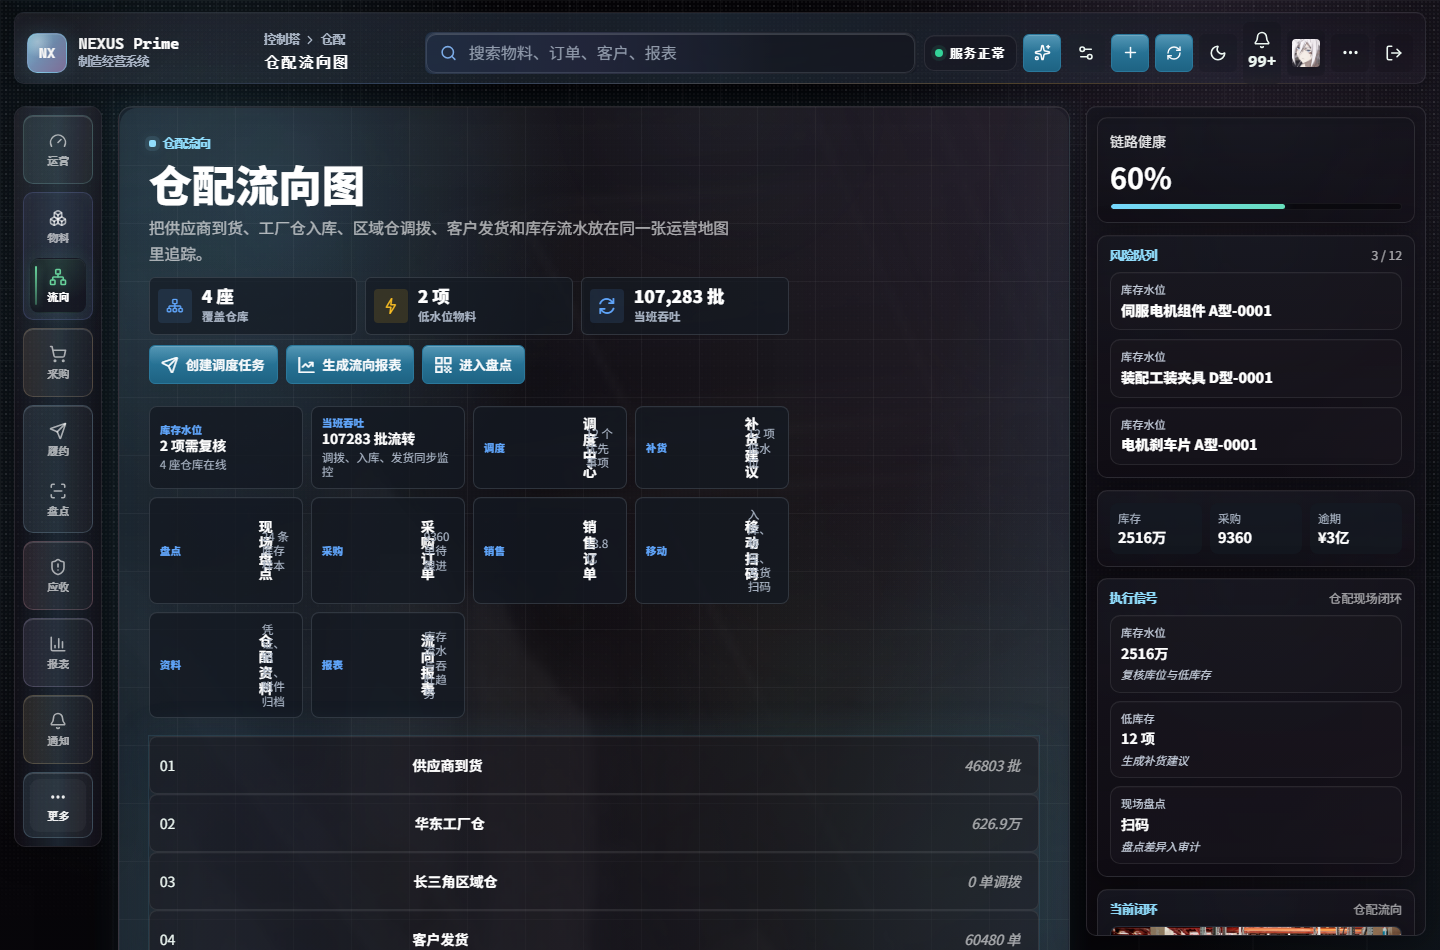
\includegraphics[width=\textwidth,height=0.38\textheight,keepaspectratio]{images/final/pages/desktop-dark-cockpit-inventory-stock.png}
  \caption{仓配流向图桌面截图，深色驾驶舱}
\end{figure}
\begin{tabularx}{\textwidth}{>{\bfseries}p{0.16\textwidth}X>{\bfseries}p{0.16\textwidth}X}
\toprule
路由 & \code{/app/inventory/stock} & 展示主题 & 深色驾驶舱 \\
主要数据 & 仓库、库存数量、库存日志、库存移动和预警。 & 主要接口 & \code{stocks, warehouses, inventory/adjust} \\
代码关联 & \multicolumn{3}{p{0.7\textwidth}}{\small ResourceWorkbench + inventory/adjust + warehouse-flow.page.ts} \\
\bottomrule
\end{tabularx}
\vspace{0.5em}
\tightpara{\textbf{页面定位：}仓配流向图展示仓库、库存数量、调拨流向和库存动作。}
\tightpara{\textbf{升级效果：}仓配域围绕物料、库存、仓库、库位、扫码和盘点。上方看库存真实场景和流向，中间看交互报表，下方用统一操作台处理库存变动、分页和记录检查。本页按照“真实图和关键图表在上、交互报表在中、表单和分页操作台在下”的规则整理，减少无意义跳转方框，让业务动作和数据对象保持同一条线。}
\begin{multicols}{2}
\textbf{主要功能}
\begin{itemize}
  \item 查看仓库和库存流向
  \item 查看库存明细和分页
  \item 执行库存调整和仓配调度
\end{itemize}
\columnbreak
\textbf{验收关注}
\begin{itemize}
  \item 上方区域优先展示真实图、态势图和关键指标，不再堆叠重复入口。
  \item 下方操作台承担搜索、分页、创建、编辑、删除、导出和领域动作。
  \item 页面跳转由 Dock、顶部搜索和资源操作台统一管理，避免随机跳转。
\end{itemize}
\end{multicols}
\clearpage
\subsection{6. 采购补货建议}
\begin{figure}[H]
  \centering
  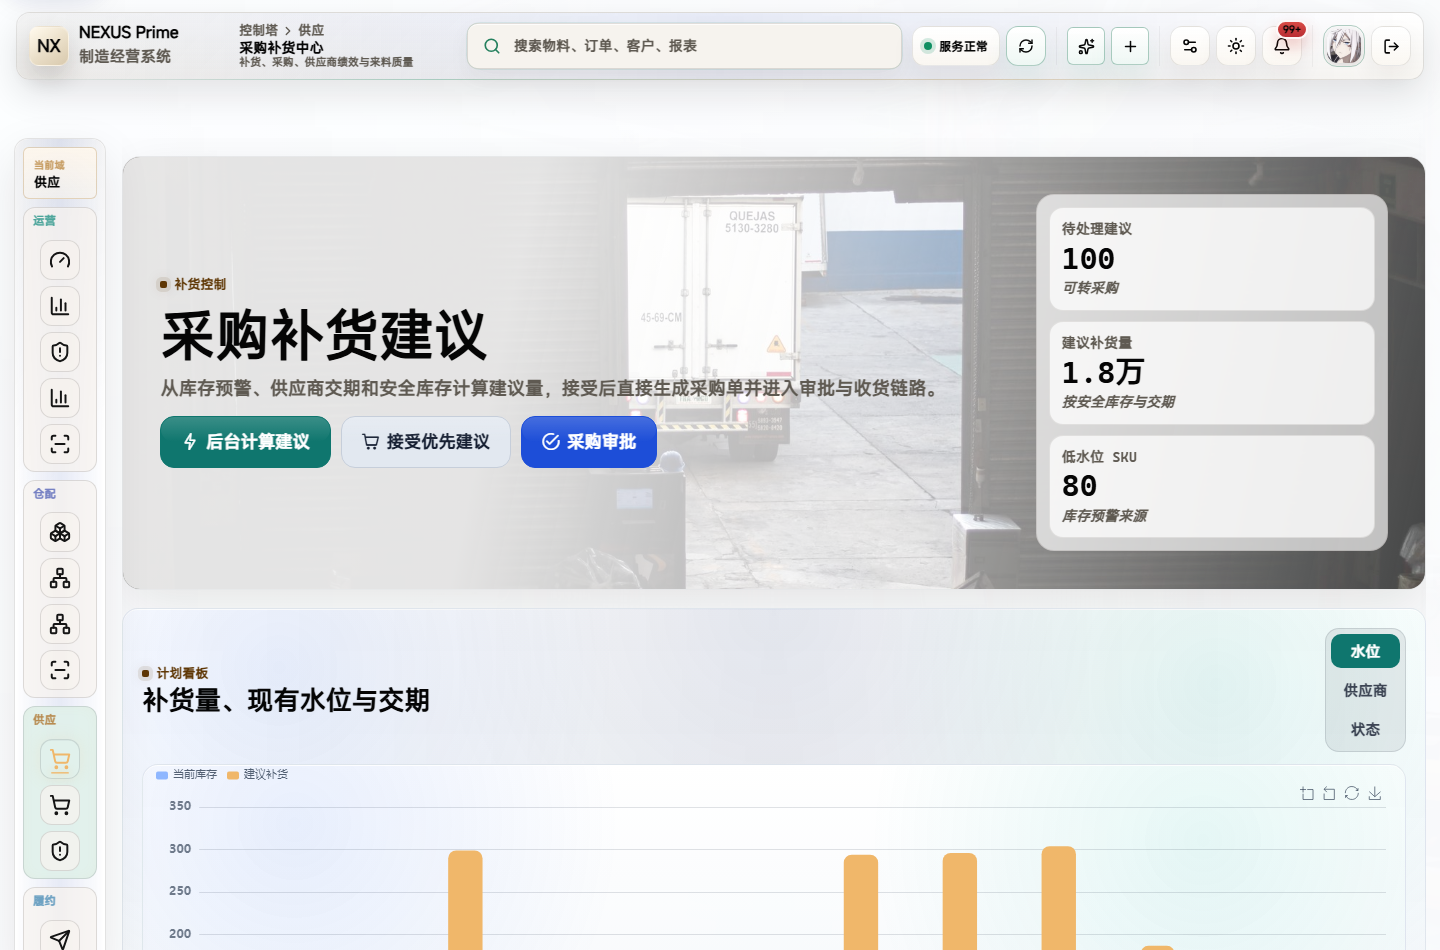
\includegraphics[width=\textwidth,height=0.38\textheight,keepaspectratio]{images/final/pages/desktop-light-luxury-inventory-replenishment.png}
  \caption{采购补货建议桌面截图，亮色系统}
\end{figure}
\begin{tabularx}{\textwidth}{>{\bfseries}p{0.16\textwidth}X>{\bfseries}p{0.16\textwidth}X}
\toprule
路由 & \code{/app/inventory/replenishment} & 展示主题 & 亮色系统 \\
主要数据 & 补货建议、商品、仓库、供应商和采购单。 & 主要接口 & \code{inventory/replenishment-suggestions} \\
代码关联 & \multicolumn{3}{p{0.7\textwidth}}{\small ResourceWorkbench + replenishment-suggestions + replenishment.page.ts} \\
\bottomrule
\end{tabularx}
\vspace{0.5em}
\tightpara{\textbf{页面定位：}采购补货建议把低库存商品、建议数量、供应商和采购转化关系放在同一页。}
\tightpara{\textbf{升级效果：}供应域连接补货建议、采购订单、供应商绩效和质量检验。核心逻辑是从低库存到采购、从采购到收货、从收货结果到供应商评分。本页按照“真实图和关键图表在上、交互报表在中、表单和分页操作台在下”的规则整理，减少无意义跳转方框，让业务动作和数据对象保持同一条线。}
\begin{multicols}{2}
\textbf{主要功能}
\begin{itemize}
  \item 生成补货建议
  \item 接受或忽略建议
  \item 跟踪建议到采购订单的转化
\end{itemize}
\columnbreak
\textbf{验收关注}
\begin{itemize}
  \item 上方区域优先展示真实图、态势图和关键指标，不再堆叠重复入口。
  \item 下方操作台承担搜索、分页、创建、编辑、删除、导出和领域动作。
  \item 页面跳转由 Dock、顶部搜索和资源操作台统一管理，避免随机跳转。
\end{itemize}
\end{multicols}
\clearpage
\subsection{7. 客户窗口与发货调度台}
\begin{figure}[H]
  \centering
  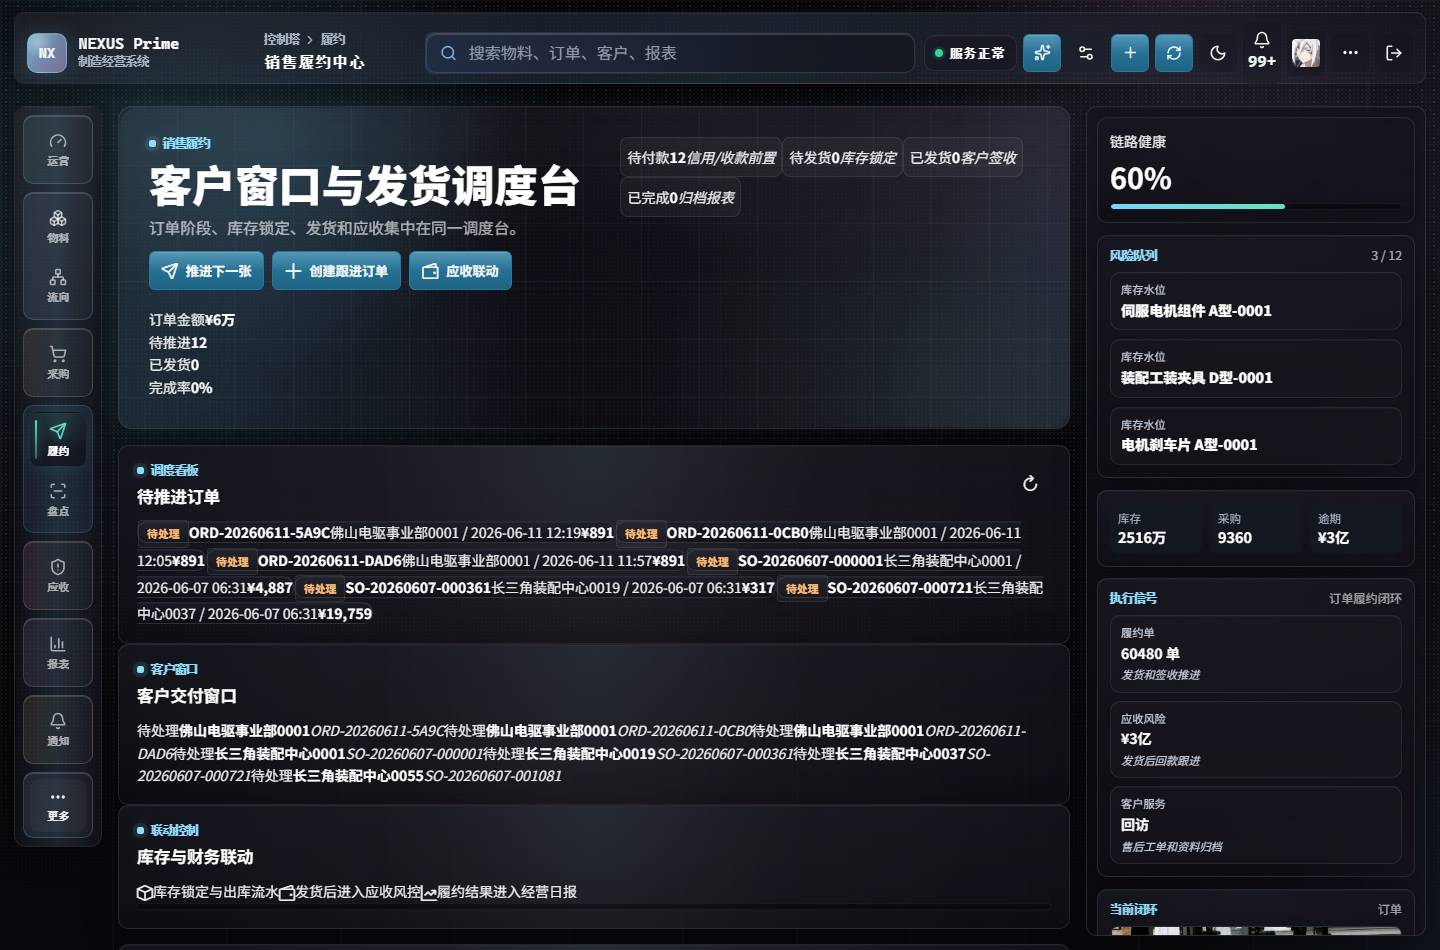
\includegraphics[width=\textwidth,height=0.38\textheight,keepaspectratio]{images/final/pages/desktop-dark-cockpit-sales-orders.png}
  \caption{客户窗口与发货调度台桌面截图，深色驾驶舱}
\end{figure}
\begin{tabularx}{\textwidth}{>{\bfseries}p{0.16\textwidth}X>{\bfseries}p{0.16\textwidth}X}
\toprule
路由 & \code{/app/sales/orders} & 展示主题 & 深色驾驶舱 \\
主要数据 & 销售订单、订单明细、客户、销售员、应收。 & 主要接口 & \code{sales/orders, sales/orders/:id/transition} \\
代码关联 & \multicolumn{3}{p{0.7\textwidth}}{\small ResourceWorkbench + sales/orders transition + fulfillment.page.ts} \\
\bottomrule
\end{tabularx}
\vspace{0.5em}
\tightpara{\textbf{页面定位：}销售履约中心管理客户订单、发货状态、销售人员和应收联动。}
\tightpara{\textbf{升级效果：}履约域连接客户、销售订单、仓配调度和售后服务。页面重点不是孤立订单表，而是展示客户价值、履约阶段、发货动作和服务闭环。本页按照“真实图和关键图表在上、交互报表在中、表单和分页操作台在下”的规则整理，减少无意义跳转方框，让业务动作和数据对象保持同一条线。}
\begin{multicols}{2}
\textbf{主要功能}
\begin{itemize}
  \item 创建和查看销售订单
  \item 推进订单状态
  \item 查看客户和商品明细
\end{itemize}
\columnbreak
\textbf{验收关注}
\begin{itemize}
  \item 上方区域优先展示真实图、态势图和关键指标，不再堆叠重复入口。
  \item 下方操作台承担搜索、分页、创建、编辑、删除、导出和领域动作。
  \item 页面跳转由 Dock、顶部搜索和资源操作台统一管理，避免随机跳转。
\end{itemize}
\end{multicols}
\clearpage
\subsection{8. 采购协同控制台}
\begin{figure}[H]
  \centering
  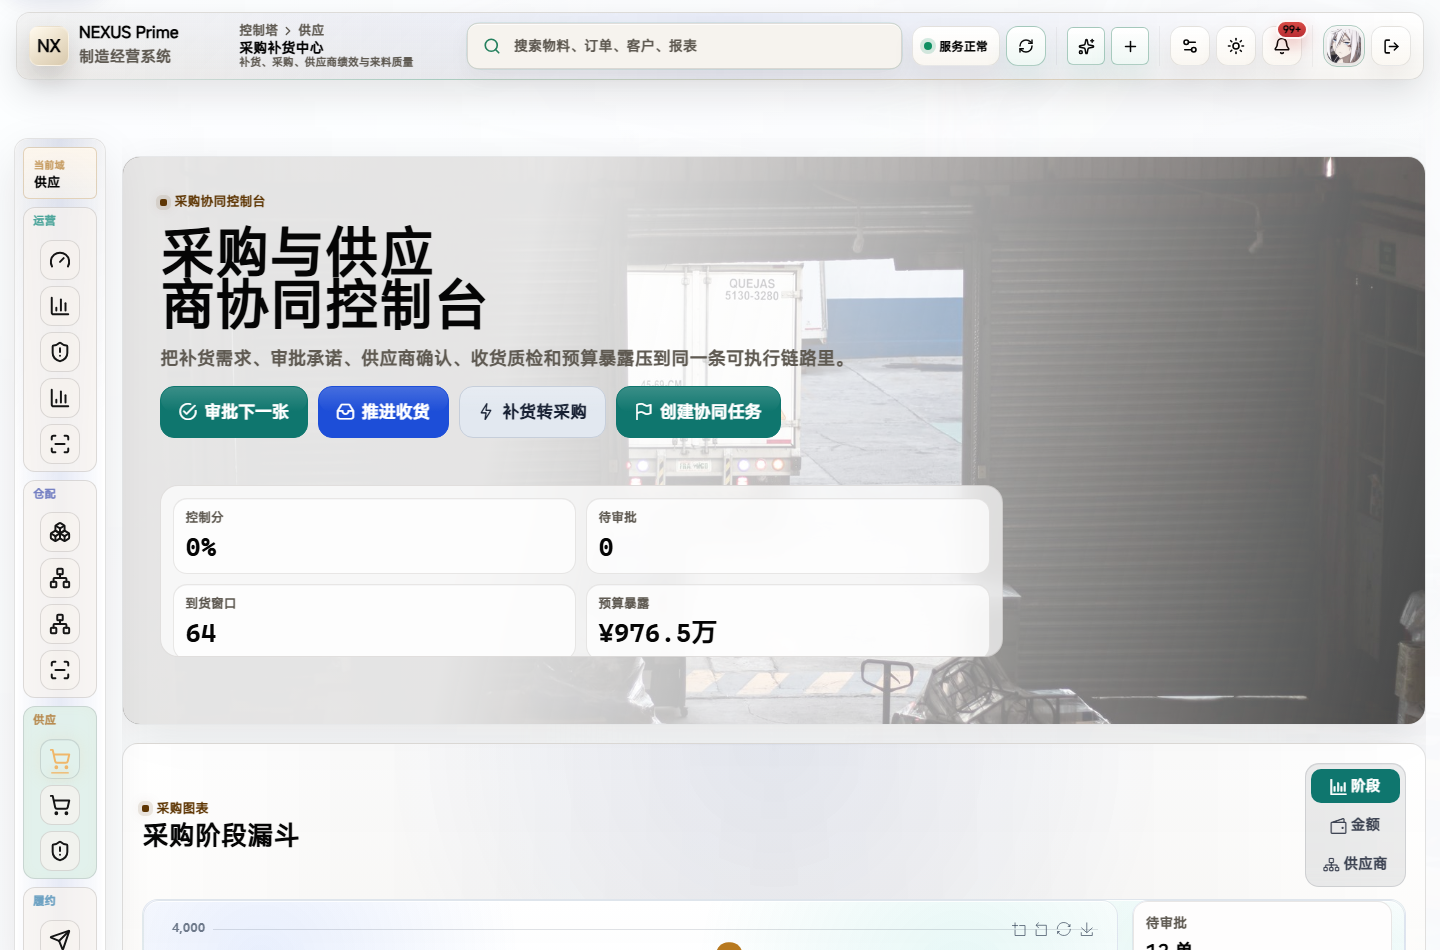
\includegraphics[width=\textwidth,height=0.38\textheight,keepaspectratio]{images/final/pages/desktop-light-luxury-procurement-orders.png}
  \caption{采购协同控制台桌面截图，亮色系统}
\end{figure}
\begin{tabularx}{\textwidth}{>{\bfseries}p{0.16\textwidth}X>{\bfseries}p{0.16\textwidth}X}
\toprule
路由 & \code{/app/procurement/orders} & 展示主题 & 亮色系统 \\
主要数据 & 采购订单、采购明细、供应商、仓库和补货建议。 & 主要接口 & \code{procurement/orders, operations/procurement-control} \\
代码关联 & \multicolumn{3}{p{0.7\textwidth}}{\small ResourceWorkbench + procurement workflow + procurement.page.ts} \\
\bottomrule
\end{tabularx}
\vspace{0.5em}
\tightpara{\textbf{页面定位：}采购协同控制台覆盖采购创建、提交、审批、收货和供应商承诺。}
\tightpara{\textbf{升级效果：}供应域连接补货建议、采购订单、供应商绩效和质量检验。核心逻辑是从低库存到采购、从采购到收货、从收货结果到供应商评分。本页按照“真实图和关键图表在上、交互报表在中、表单和分页操作台在下”的规则整理，减少无意义跳转方框，让业务动作和数据对象保持同一条线。}
\begin{multicols}{2}
\textbf{主要功能}
\begin{itemize}
  \item 查看采购订单
  \item 提交审批和批准
  \item 登记收货并跟踪采购进度
\end{itemize}
\columnbreak
\textbf{验收关注}
\begin{itemize}
  \item 上方区域优先展示真实图、态势图和关键指标，不再堆叠重复入口。
  \item 下方操作台承担搜索、分页、创建、编辑、删除、导出和领域动作。
  \item 页面跳转由 Dock、顶部搜索和资源操作台统一管理，避免随机跳转。
\end{itemize}
\end{multicols}
\clearpage
\subsection{9. 供应商协同}
\begin{figure}[H]
  \centering
  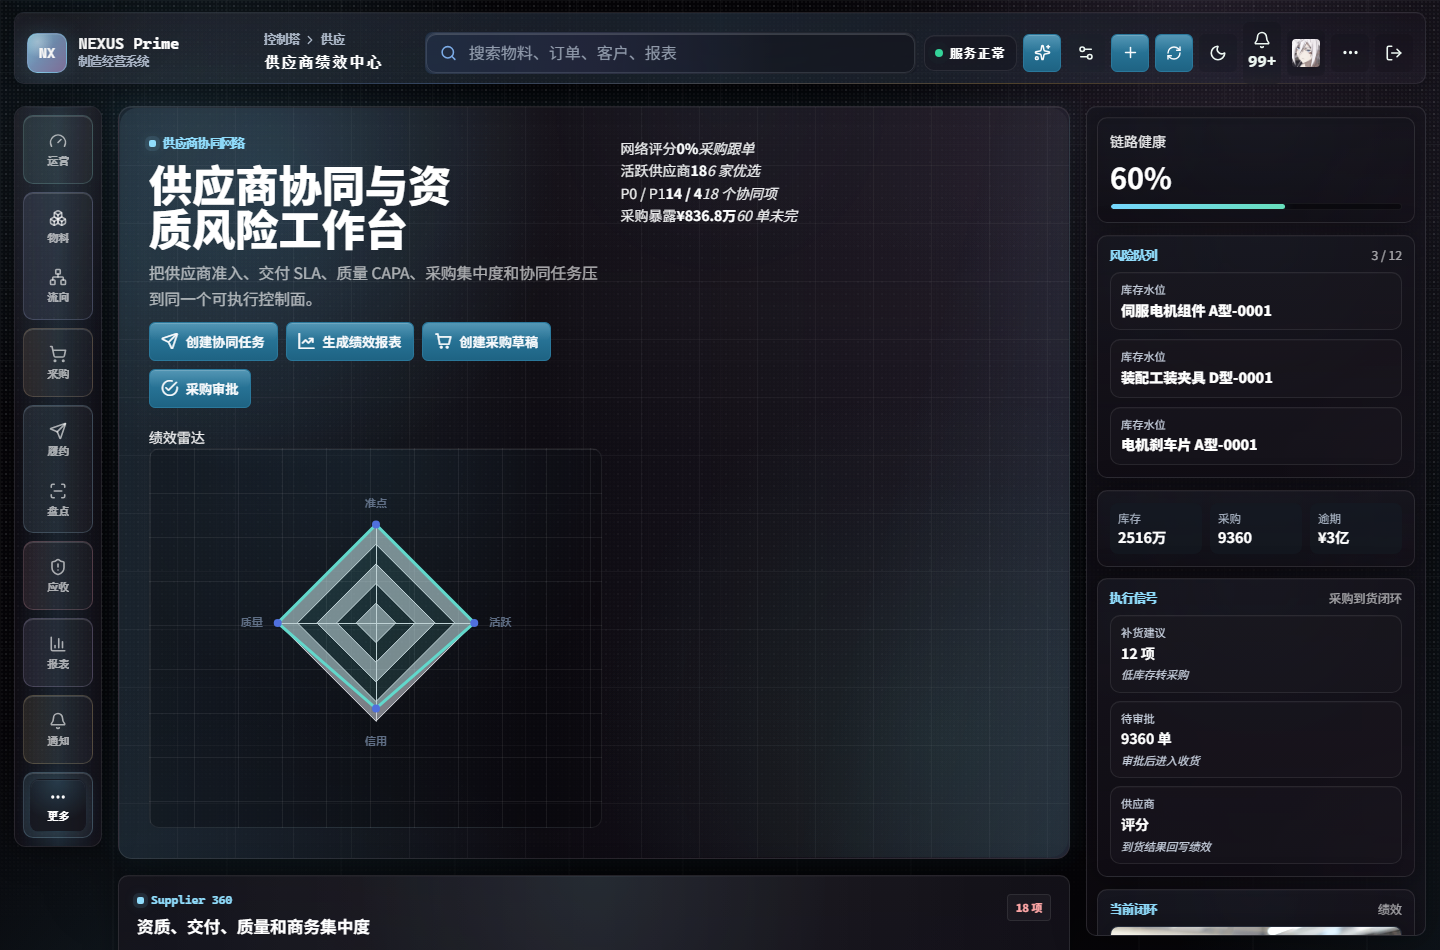
\includegraphics[width=\textwidth,height=0.38\textheight,keepaspectratio]{images/final/pages/desktop-dark-cockpit-suppliers-performance.png}
  \caption{供应商协同桌面截图，深色驾驶舱}
\end{figure}
\begin{tabularx}{\textwidth}{>{\bfseries}p{0.16\textwidth}X>{\bfseries}p{0.16\textwidth}X}
\toprule
路由 & \code{/app/suppliers/performance} & 展示主题 & 深色驾驶舱 \\
主要数据 & 供应商绩效、伙伴档案、采购订单和质量指标。 & 主要接口 & \code{suppliers-performance, partners} \\
代码关联 & \multicolumn{3}{p{0.7\textwidth}}{\small supplier-performance.page.ts + supplier\_performance 模型} \\
\bottomrule
\end{tabularx}
\vspace{0.5em}
\tightpara{\textbf{页面定位：}供应商协同网络评估供应商交付、质量、信用和待办采购风险。}
\tightpara{\textbf{升级效果：}供应域连接补货建议、采购订单、供应商绩效和质量检验。核心逻辑是从低库存到采购、从采购到收货、从收货结果到供应商评分。本页按照“真实图和关键图表在上、交互报表在中、表单和分页操作台在下”的规则整理，减少无意义跳转方框，让业务动作和数据对象保持同一条线。}
\begin{multicols}{2}
\textbf{主要功能}
\begin{itemize}
  \item 查看供应商绩效
  \item 识别延期和质量风险
  \item 联动采购订单和补货任务
\end{itemize}
\columnbreak
\textbf{验收关注}
\begin{itemize}
  \item 上方区域优先展示真实图、态势图和关键指标，不再堆叠重复入口。
  \item 下方操作台承担搜索、分页、创建、编辑、删除、导出和领域动作。
  \item 页面跳转由 Dock、顶部搜索和资源操作台统一管理，避免随机跳转。
\end{itemize}
\end{multicols}
\clearpage
\subsection{10. 仓配调度中心}
\begin{figure}[H]
  \centering
  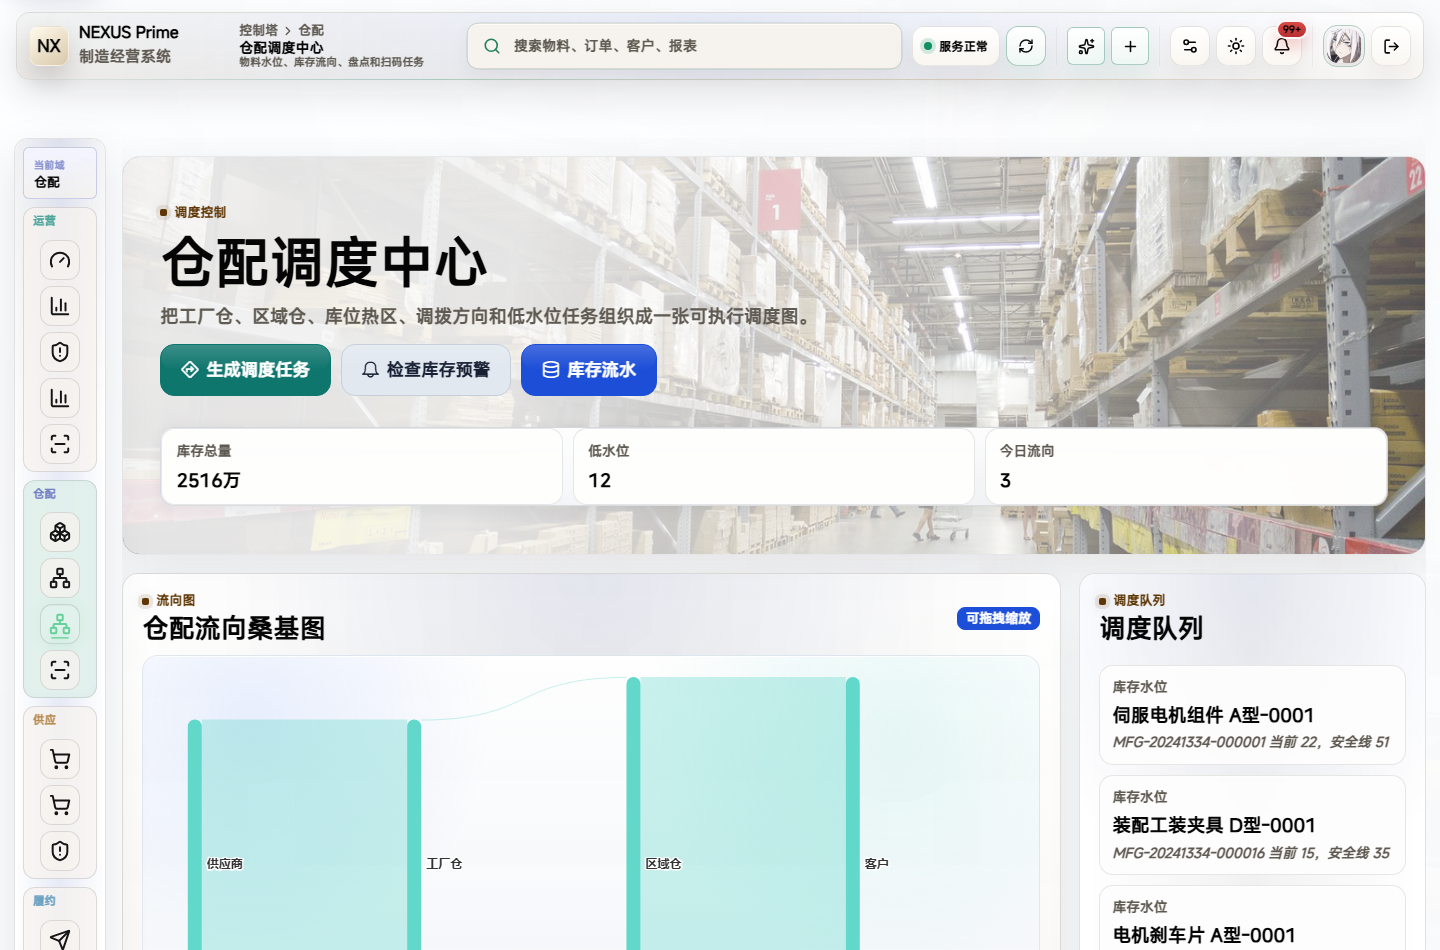
\includegraphics[width=\textwidth,height=0.38\textheight,keepaspectratio]{images/final/pages/desktop-light-luxury-dispatch.png}
  \caption{仓配调度中心桌面截图，亮色系统}
\end{figure}
\begin{tabularx}{\textwidth}{>{\bfseries}p{0.16\textwidth}X>{\bfseries}p{0.16\textwidth}X}
\toprule
路由 & \code{/app/dispatch} & 展示主题 & 亮色系统 \\
主要数据 & 仓库、库存流水、任务队列和异常提示。 & 主要接口 & \code{operations/dispatch, stocks, stock-logs} \\
代码关联 & \multicolumn{3}{p{0.7\textwidth}}{\small dispatch-center.page.ts + operations/dispatch} \\
\bottomrule
\end{tabularx}
\vspace{0.5em}
\tightpara{\textbf{页面定位：}仓配调度中心聚焦仓库负载、出入库节奏和调度任务。}
\tightpara{\textbf{升级效果：}仓配域围绕物料、库存、仓库、库位、扫码和盘点。上方看库存真实场景和流向，中间看交互报表，下方用统一操作台处理库存变动、分页和记录检查。本页按照“真实图和关键图表在上、交互报表在中、表单和分页操作台在下”的规则整理，减少无意义跳转方框，让业务动作和数据对象保持同一条线。}
\begin{multicols}{2}
\textbf{主要功能}
\begin{itemize}
  \item 查看仓配任务
  \item 识别拥堵仓库
  \item 跟踪执行队列和调度建议
\end{itemize}
\columnbreak
\textbf{验收关注}
\begin{itemize}
  \item 上方区域优先展示真实图、态势图和关键指标，不再堆叠重复入口。
  \item 下方操作台承担搜索、分页、创建、编辑、删除、导出和领域动作。
  \item 页面跳转由 Dock、顶部搜索和资源操作台统一管理，避免随机跳转。
\end{itemize}
\end{multicols}
\clearpage
\subsection{11. 数据质量中心}
\begin{figure}[H]
  \centering
  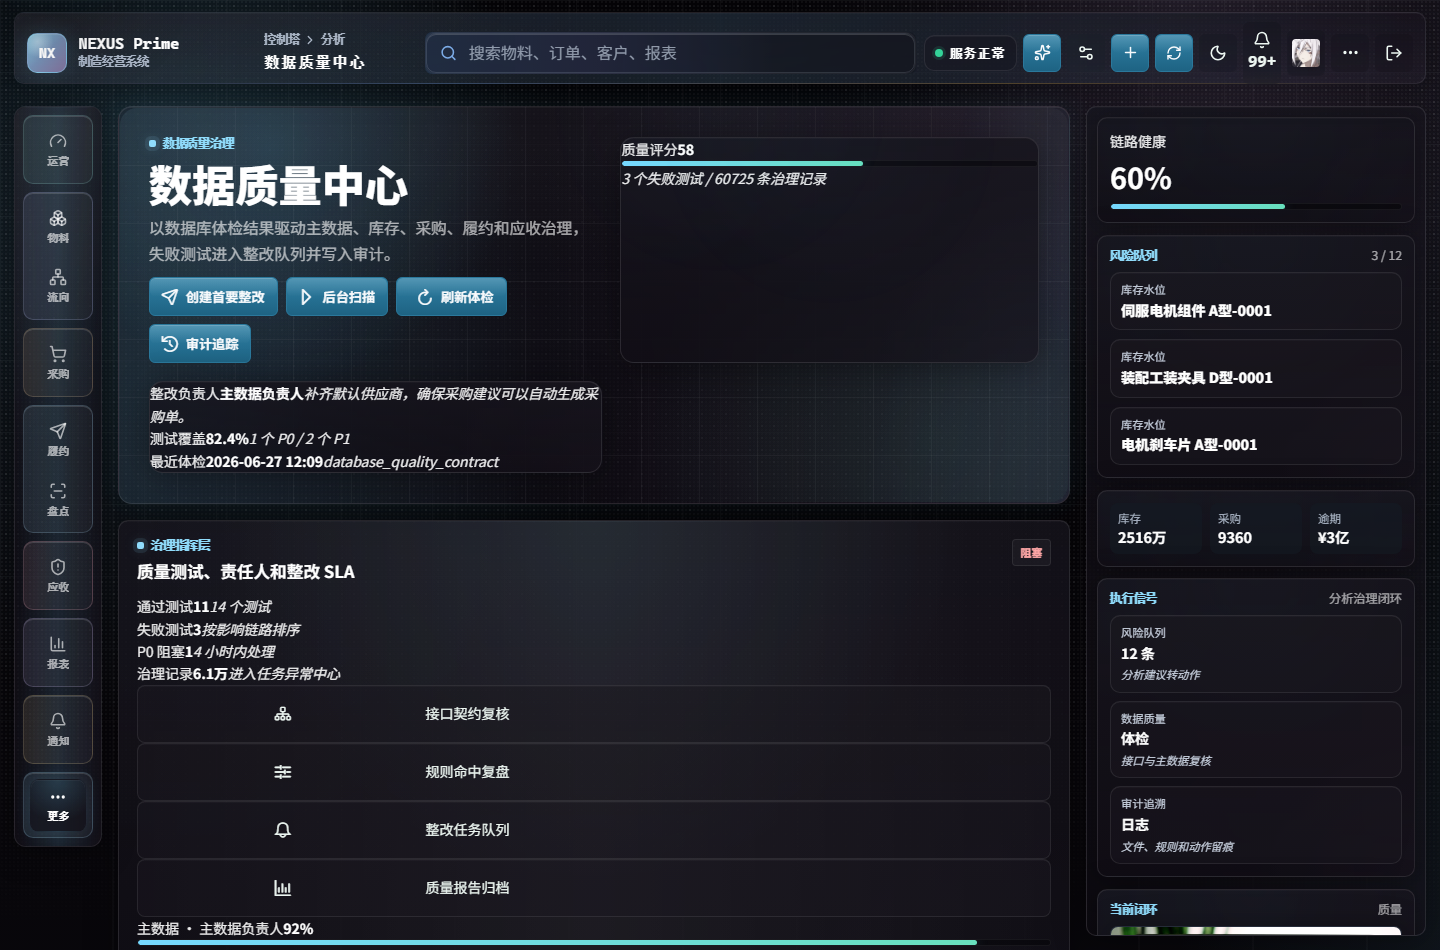
\includegraphics[width=\textwidth,height=0.38\textheight,keepaspectratio]{images/final/pages/desktop-dark-cockpit-data-quality.png}
  \caption{数据质量中心桌面截图，深色驾驶舱}
\end{figure}
\begin{tabularx}{\textwidth}{>{\bfseries}p{0.16\textwidth}X>{\bfseries}p{0.16\textwidth}X}
\toprule
路由 & \code{/app/data-quality} & 展示主题 & 深色驾驶舱 \\
主要数据 & 商品、伙伴、订单、库存和审计检查结果。 & 主要接口 & \code{operations/data-quality} \\
代码关联 & \multicolumn{3}{p{0.7\textwidth}}{\small data-quality.page.ts + data quality jobs} \\
\bottomrule
\end{tabularx}
\vspace{0.5em}
\tightpara{\textbf{页面定位：}数据质量中心用于检查主数据完整性、重复记录和业务字段异常。}
\tightpara{\textbf{升级效果：}分析域覆盖报表、规则、数据质量、集成和 AI。它把系统状态、数据可信度和经营建议放到一套分析流程里。本页按照“真实图和关键图表在上、交互报表在中、表单和分页操作台在下”的规则整理，减少无意义跳转方框，让业务动作和数据对象保持同一条线。}
\begin{multicols}{2}
\textbf{主要功能}
\begin{itemize}
  \item 查看数据质量评分
  \item 定位缺失字段
  \item 跟踪修复任务
\end{itemize}
\columnbreak
\textbf{验收关注}
\begin{itemize}
  \item 上方区域优先展示真实图、态势图和关键指标，不再堆叠重复入口。
  \item 下方操作台承担搜索、分页、创建、编辑、删除、导出和领域动作。
  \item 页面跳转由 Dock、顶部搜索和资源操作台统一管理，避免随机跳转。
\end{itemize}
\end{multicols}
\clearpage
\subsection{12. 质量检验中心}
\begin{figure}[H]
  \centering
  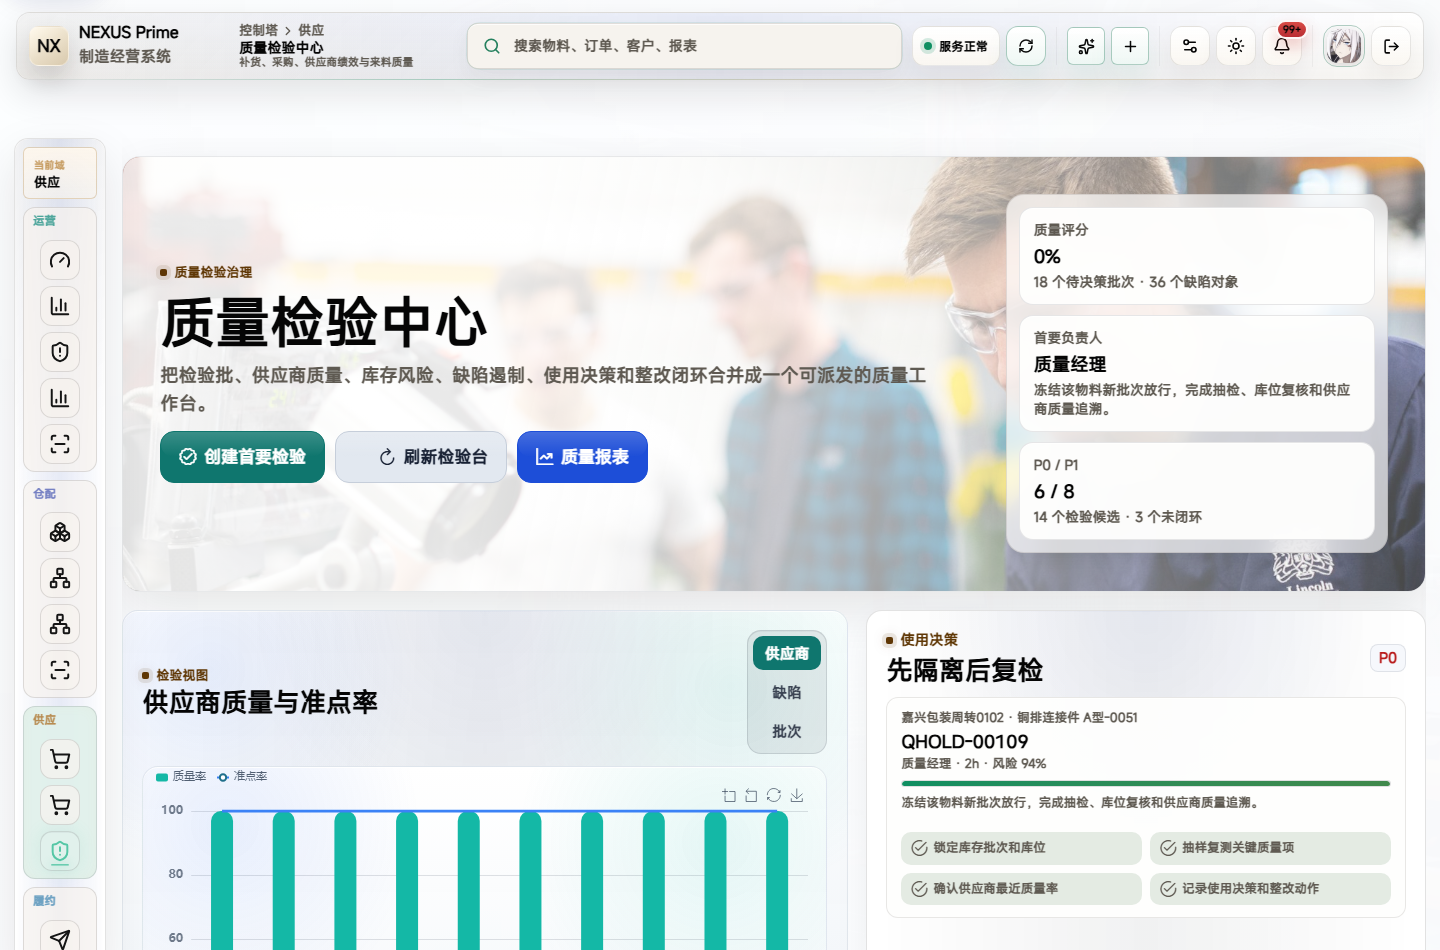
\includegraphics[width=\textwidth,height=0.38\textheight,keepaspectratio]{images/final/pages/desktop-light-luxury-quality.png}
  \caption{质量检验中心桌面截图，亮色系统}
\end{figure}
\begin{tabularx}{\textwidth}{>{\bfseries}p{0.16\textwidth}X>{\bfseries}p{0.16\textwidth}X}
\toprule
路由 & \code{/app/quality} & 展示主题 & 亮色系统 \\
主要数据 & 质量任务、采购、供应商、商品和异常记录。 & 主要接口 & \code{operations/quality-inspection} \\
代码关联 & \multicolumn{3}{p{0.7\textwidth}}{\small quality-inspection.page.ts + operations/quality-inspection} \\
\bottomrule
\end{tabularx}
\vspace{0.5em}
\tightpara{\textbf{页面定位：}质量检验中心管理检验批、质量问题、处置动作和质量趋势。}
\tightpara{\textbf{升级效果：}供应域连接补货建议、采购订单、供应商绩效和质量检验。核心逻辑是从低库存到采购、从采购到收货、从收货结果到供应商评分。本页按照“真实图和关键图表在上、交互报表在中、表单和分页操作台在下”的规则整理，减少无意义跳转方框，让业务动作和数据对象保持同一条线。}
\begin{multicols}{2}
\textbf{主要功能}
\begin{itemize}
  \item 查看检验任务
  \item 记录质量处置
  \item 识别供应商和产品质量风险
\end{itemize}
\columnbreak
\textbf{验收关注}
\begin{itemize}
  \item 上方区域优先展示真实图、态势图和关键指标，不再堆叠重复入口。
  \item 下方操作台承担搜索、分页、创建、编辑、删除、导出和领域动作。
  \item 页面跳转由 Dock、顶部搜索和资源操作台统一管理，避免随机跳转。
\end{itemize}
\end{multicols}
\clearpage
\subsection{13. 客户经营中心}
\begin{figure}[H]
  \centering
  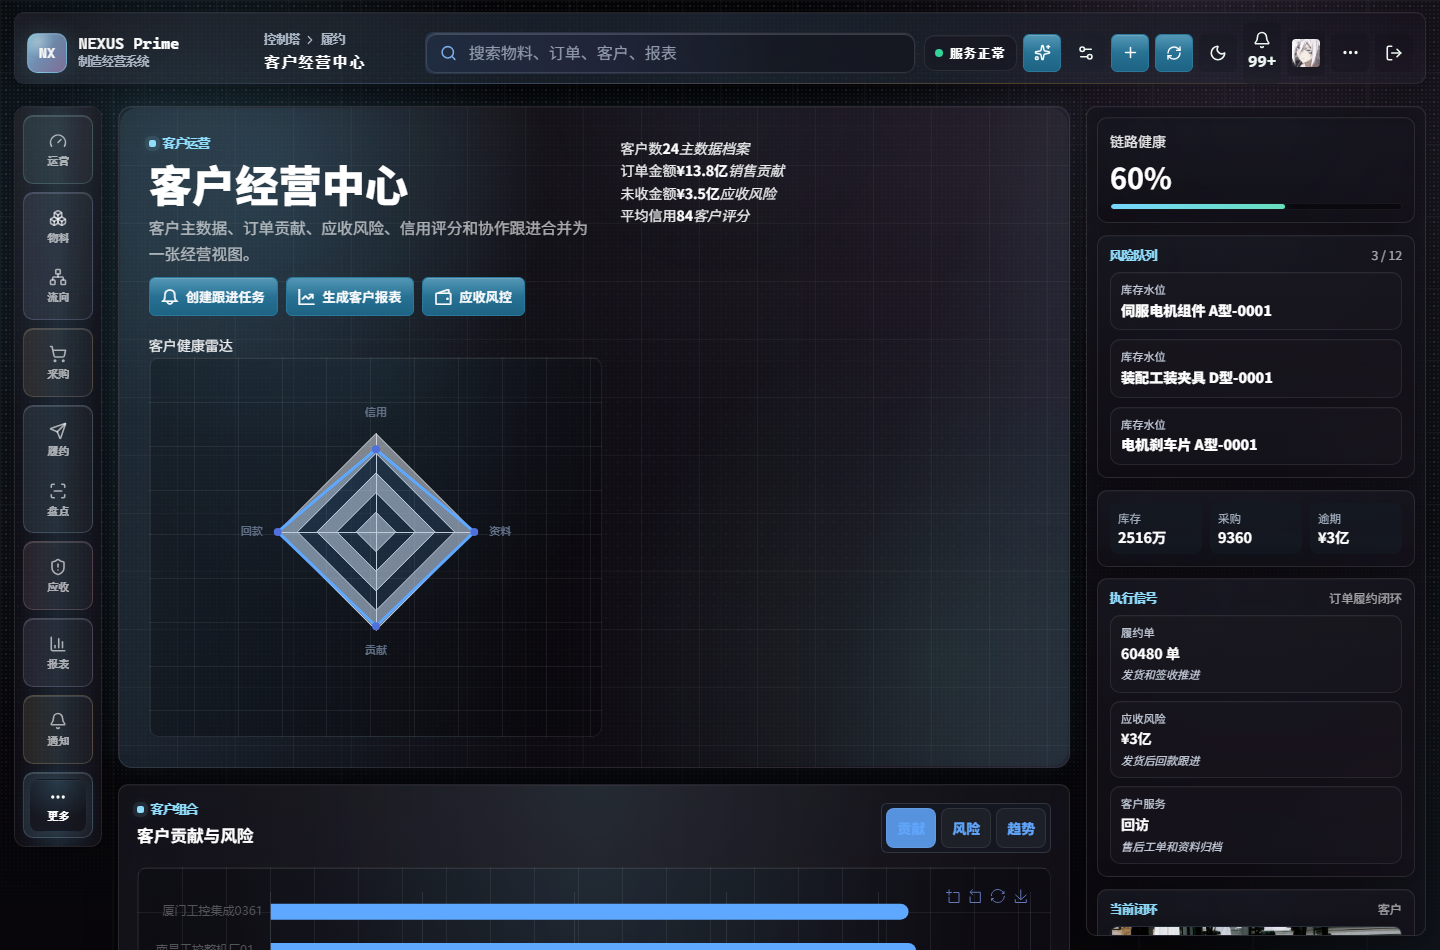
\includegraphics[width=\textwidth,height=0.38\textheight,keepaspectratio]{images/final/pages/desktop-dark-cockpit-customers.png}
  \caption{客户经营中心桌面截图，深色驾驶舱}
\end{figure}
\begin{tabularx}{\textwidth}{>{\bfseries}p{0.16\textwidth}X>{\bfseries}p{0.16\textwidth}X}
\toprule
路由 & \code{/app/customers} & 展示主题 & 深色驾驶舱 \\
主要数据 & 客户伙伴、订单、应收、信用和服务记录。 & 主要接口 & \code{partners, sales/orders, finance/credits} \\
代码关联 & \multicolumn{3}{p{0.7\textwidth}}{\small ResourceWorkbench + partners 资源配置 + customer-operations.page.ts} \\
\bottomrule
\end{tabularx}
\vspace{0.5em}
\tightpara{\textbf{页面定位：}客户经营中心把客户档案、交易贡献、风险和服务动作合并展示。}
\tightpara{\textbf{升级效果：}履约域连接客户、销售订单、仓配调度和售后服务。页面重点不是孤立订单表，而是展示客户价值、履约阶段、发货动作和服务闭环。本页按照“真实图和关键图表在上、交互报表在中、表单和分页操作台在下”的规则整理，减少无意义跳转方框，让业务动作和数据对象保持同一条线。}
\begin{multicols}{2}
\textbf{主要功能}
\begin{itemize}
  \item 查看客户清单
  \item 识别高价值和高风险客户
  \item 进入订单、应收和信用动作
\end{itemize}
\columnbreak
\textbf{验收关注}
\begin{itemize}
  \item 上方区域优先展示真实图、态势图和关键指标，不再堆叠重复入口。
  \item 下方操作台承担搜索、分页、创建、编辑、删除、导出和领域动作。
  \item 页面跳转由 Dock、顶部搜索和资源操作台统一管理，避免随机跳转。
\end{itemize}
\end{multicols}
\clearpage
\subsection{14. 产能计划中心}
\begin{figure}[H]
  \centering
  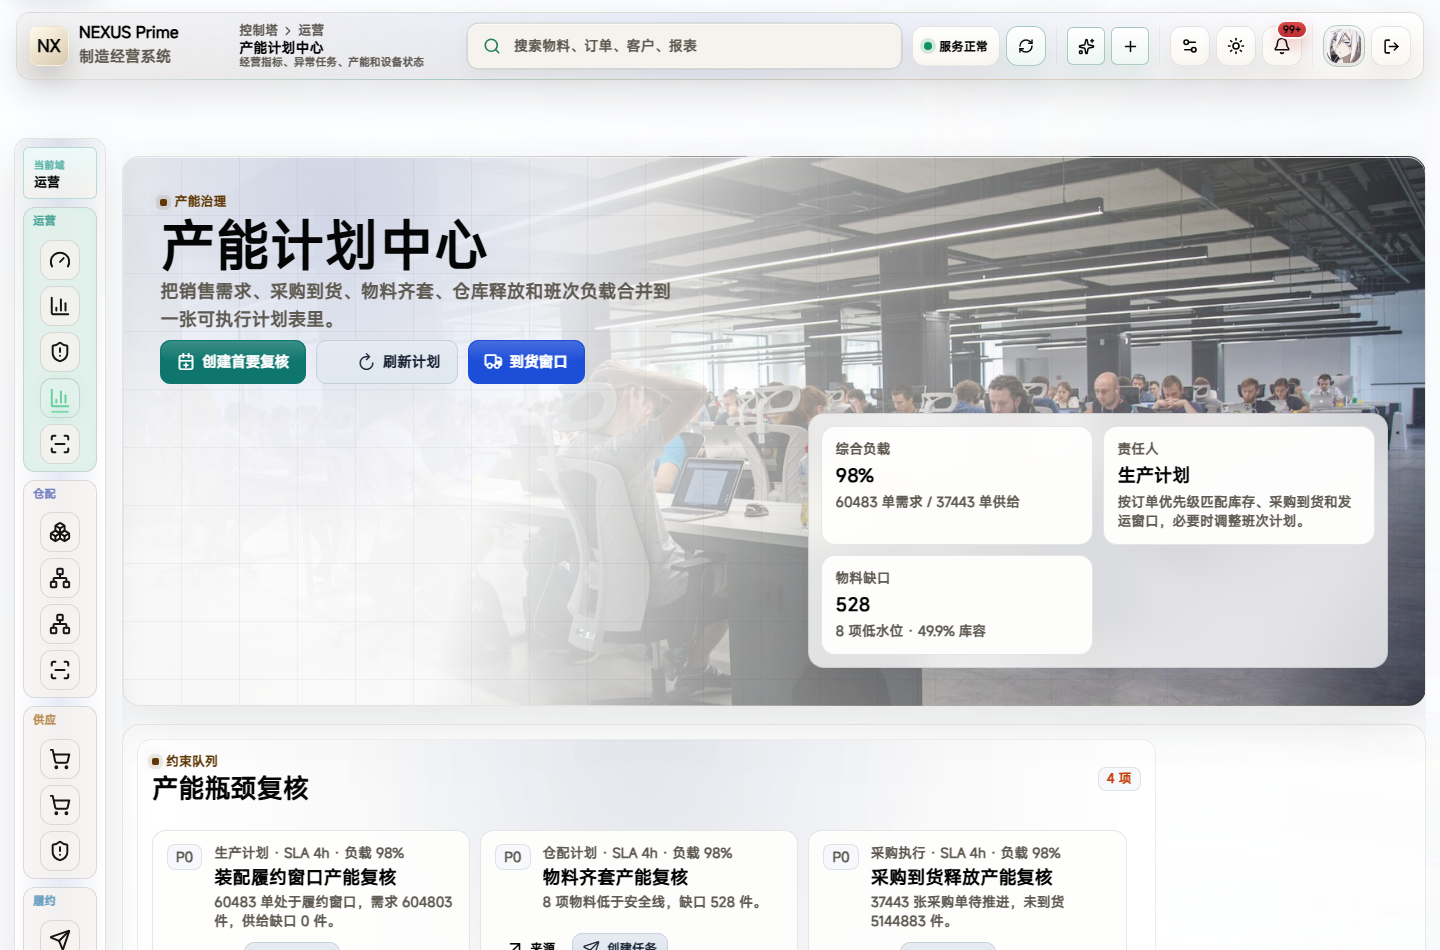
\includegraphics[width=\textwidth,height=0.38\textheight,keepaspectratio]{images/final/pages/desktop-light-luxury-capacity.png}
  \caption{产能计划中心桌面截图，亮色系统}
\end{figure}
\begin{tabularx}{\textwidth}{>{\bfseries}p{0.16\textwidth}X>{\bfseries}p{0.16\textwidth}X}
\toprule
路由 & \code{/app/capacity} & 展示主题 & 亮色系统 \\
主要数据 & 产能计划、设备、采购、库存和任务队列。 & 主要接口 & \code{operations/capacity, operations/capacity/review} \\
代码关联 & \multicolumn{3}{p{0.7\textwidth}}{\small capacity-planning.page.ts + operations/capacity} \\
\bottomrule
\end{tabularx}
\vspace{0.5em}
\tightpara{\textbf{页面定位：}产能计划中心用于查看产能负载、瓶颈工序、齐套风险和排产建议。}
\tightpara{\textbf{升级效果：}运营域强调经营指标、任务异常、产能和设备状态，目标是把管理者每天先看的信息放在同一层。页面不再用零散跳转块，而是以态势图、风险队列和执行列表组织。本页按照“真实图和关键图表在上、交互报表在中、表单和分页操作台在下”的规则整理，减少无意义跳转方框，让业务动作和数据对象保持同一条线。}
\begin{multicols}{2}
\textbf{主要功能}
\begin{itemize}
  \item 查看产能负载
  \item 发起产能复核
  \item 识别齐套和设备瓶颈
\end{itemize}
\columnbreak
\textbf{验收关注}
\begin{itemize}
  \item 上方区域优先展示真实图、态势图和关键指标，不再堆叠重复入口。
  \item 下方操作台承担搜索、分页、创建、编辑、删除、导出和领域动作。
  \item 页面跳转由 Dock、顶部搜索和资源操作台统一管理，避免随机跳转。
\end{itemize}
\end{multicols}
\clearpage
\subsection{15. 设备维护中心}
\begin{figure}[H]
  \centering
  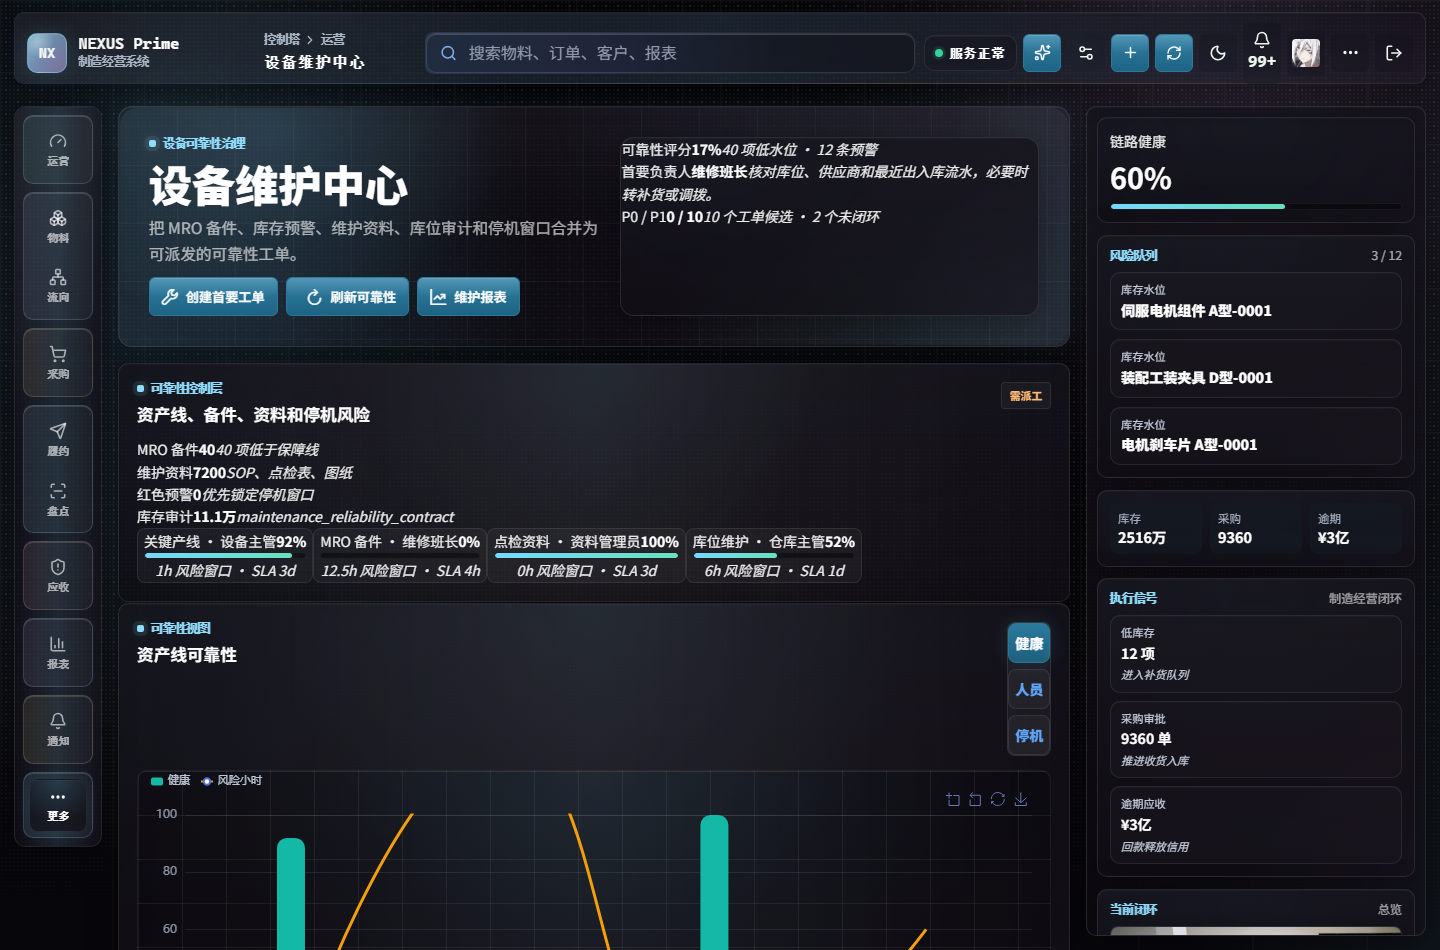
\includegraphics[width=\textwidth,height=0.38\textheight,keepaspectratio]{images/final/pages/desktop-dark-cockpit-maintenance.png}
  \caption{设备维护中心桌面截图，深色驾驶舱}
\end{figure}
\begin{tabularx}{\textwidth}{>{\bfseries}p{0.16\textwidth}X>{\bfseries}p{0.16\textwidth}X}
\toprule
路由 & \code{/app/maintenance} & 展示主题 & 深色驾驶舱 \\
主要数据 & 设备、维护工单、产能和质量异常。 & 主要接口 & \code{operations/maintenance, operations/maintenance-workorder} \\
代码关联 & \multicolumn{3}{p{0.7\textwidth}}{\small maintenance.page.ts + operations/maintenance} \\
\bottomrule
\end{tabularx}
\vspace{0.5em}
\tightpara{\textbf{页面定位：}设备维护中心用于管理设备状态、预防维护、故障工单和可靠性指标。}
\tightpara{\textbf{升级效果：}运营域强调经营指标、任务异常、产能和设备状态，目标是把管理者每天先看的信息放在同一层。页面不再用零散跳转块，而是以态势图、风险队列和执行列表组织。本页按照“真实图和关键图表在上、交互报表在中、表单和分页操作台在下”的规则整理，减少无意义跳转方框，让业务动作和数据对象保持同一条线。}
\begin{multicols}{2}
\textbf{主要功能}
\begin{itemize}
  \item 查看设备健康
  \item 创建维护工单
  \item 跟踪维修队列和停机影响
\end{itemize}
\columnbreak
\textbf{验收关注}
\begin{itemize}
  \item 上方区域优先展示真实图、态势图和关键指标，不再堆叠重复入口。
  \item 下方操作台承担搜索、分页、创建、编辑、删除、导出和领域动作。
  \item 页面跳转由 Dock、顶部搜索和资源操作台统一管理，避免随机跳转。
\end{itemize}
\end{multicols}
\clearpage
\subsection{16. 合同回款中心}
\begin{figure}[H]
  \centering
  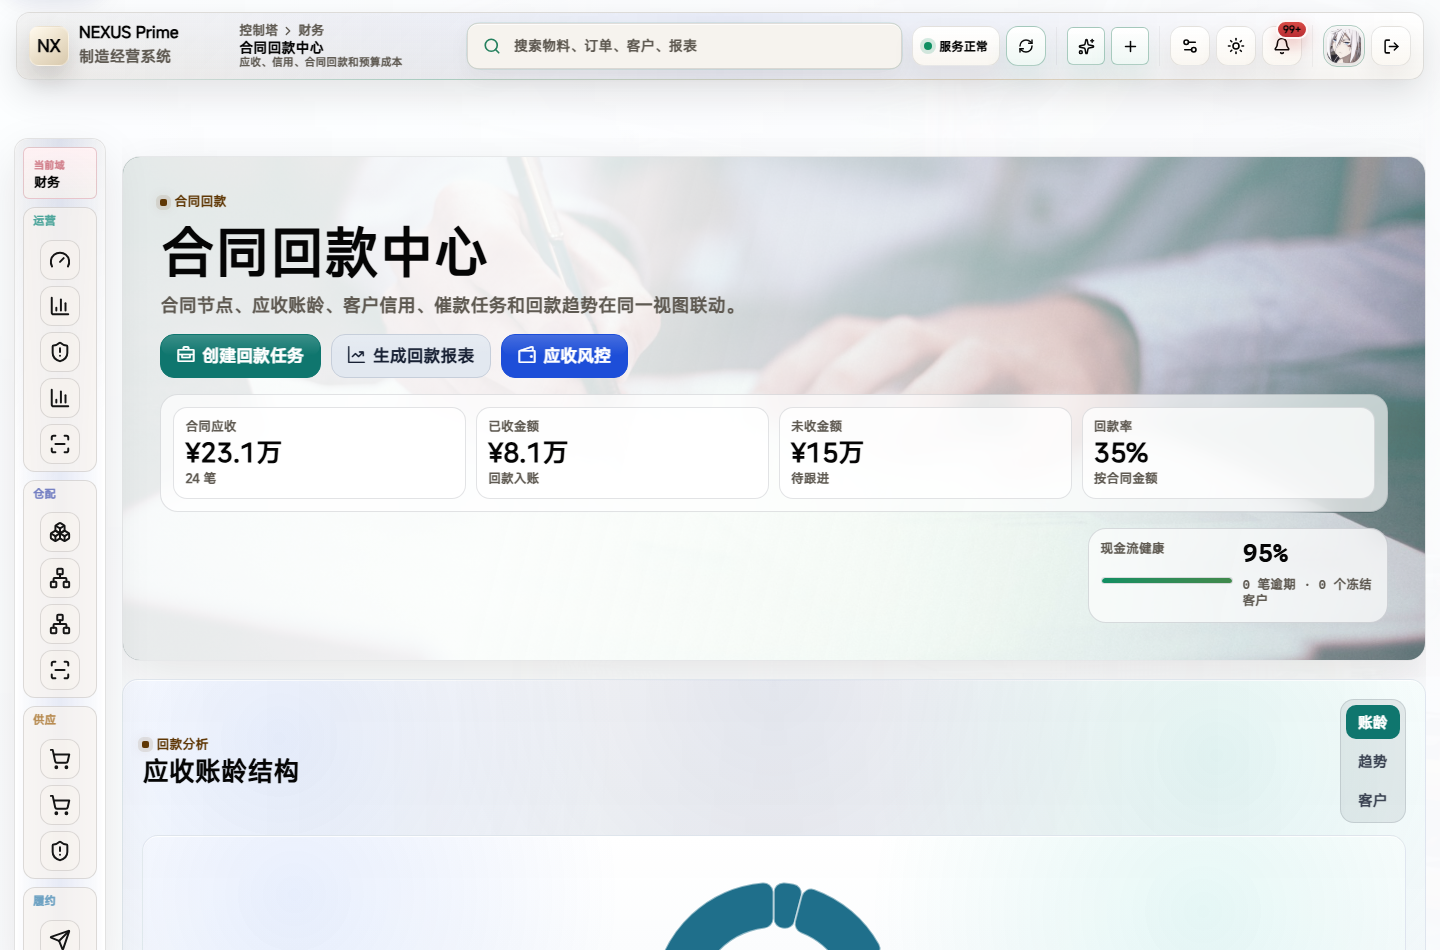
\includegraphics[width=\textwidth,height=0.38\textheight,keepaspectratio]{images/final/pages/desktop-light-luxury-contracts.png}
  \caption{合同回款中心桌面截图，亮色系统}
\end{figure}
\begin{tabularx}{\textwidth}{>{\bfseries}p{0.16\textwidth}X>{\bfseries}p{0.16\textwidth}X}
\toprule
路由 & \code{/app/contracts} & 展示主题 & 亮色系统 \\
主要数据 & 合同、销售订单、应收账款、收款记录和客户。 & 主要接口 & \code{contracts, finance/receivables} \\
代码关联 & \multicolumn{3}{p{0.7\textwidth}}{\small contract-collection.page.ts + finance/receivables} \\
\bottomrule
\end{tabularx}
\vspace{0.5em}
\tightpara{\textbf{页面定位：}合同回款中心连接合同、订单、应收和回款风险。}
\tightpara{\textbf{升级效果：}财务域覆盖应收、信用、合同和预算成本。它用账龄、额度、回款和成本偏差表达经营风险，让财务动作能回到订单、客户和合同。本页按照“真实图和关键图表在上、交互报表在中、表单和分页操作台在下”的规则整理，减少无意义跳转方框，让业务动作和数据对象保持同一条线。}
\begin{multicols}{2}
\textbf{主要功能}
\begin{itemize}
  \item 查看合同和回款节点
  \item 识别逾期风险
  \item 联动财务收款和客户信用
\end{itemize}
\columnbreak
\textbf{验收关注}
\begin{itemize}
  \item 上方区域优先展示真实图、态势图和关键指标，不再堆叠重复入口。
  \item 下方操作台承担搜索、分页、创建、编辑、删除、导出和领域动作。
  \item 页面跳转由 Dock、顶部搜索和资源操作台统一管理，避免随机跳转。
\end{itemize}
\end{multicols}
\clearpage
\subsection{17. 售后服务中心}
\begin{figure}[H]
  \centering
  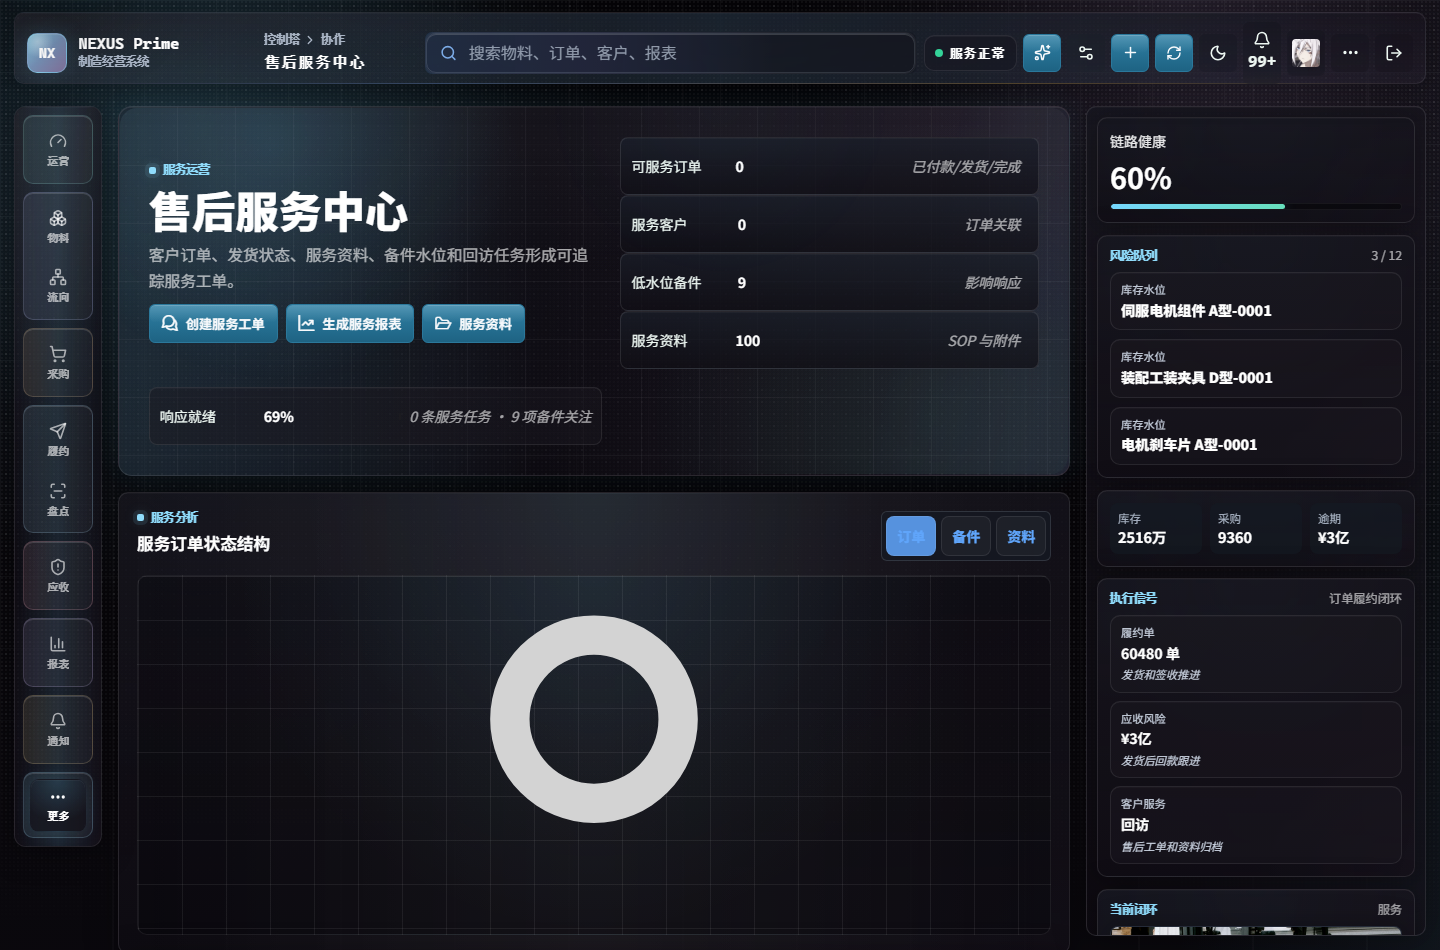
\includegraphics[width=\textwidth,height=0.38\textheight,keepaspectratio]{images/final/pages/desktop-dark-cockpit-service.png}
  \caption{售后服务中心桌面截图，深色驾驶舱}
\end{figure}
\begin{tabularx}{\textwidth}{>{\bfseries}p{0.16\textwidth}X>{\bfseries}p{0.16\textwidth}X}
\toprule
路由 & \code{/app/service} & 展示主题 & 深色驾驶舱 \\
主要数据 & 客户、订单、售后工单、质量问题和通知。 & 主要接口 & \code{operations/service, partners} \\
代码关联 & \multicolumn{3}{p{0.7\textwidth}}{\small service-workorders.page.ts + operations/service} \\
\bottomrule
\end{tabularx}
\vspace{0.5em}
\tightpara{\textbf{页面定位：}售后服务中心管理客户服务、问题处理和履约后的反馈闭环。}
\tightpara{\textbf{升级效果：}履约域连接客户、销售订单、仓配调度和售后服务。页面重点不是孤立订单表，而是展示客户价值、履约阶段、发货动作和服务闭环。本页按照“真实图和关键图表在上、交互报表在中、表单和分页操作台在下”的规则整理，减少无意义跳转方框，让业务动作和数据对象保持同一条线。}
\begin{multicols}{2}
\textbf{主要功能}
\begin{itemize}
  \item 查看服务工单
  \item 识别客户反馈风险
  \item 联动客户、订单和质量页面
\end{itemize}
\columnbreak
\textbf{验收关注}
\begin{itemize}
  \item 上方区域优先展示真实图、态势图和关键指标，不再堆叠重复入口。
  \item 下方操作台承担搜索、分页、创建、编辑、删除、导出和领域动作。
  \item 页面跳转由 Dock、顶部搜索和资源操作台统一管理，避免随机跳转。
\end{itemize}
\end{multicols}
\clearpage
\subsection{18. 规则引擎中心}
\begin{figure}[H]
  \centering
  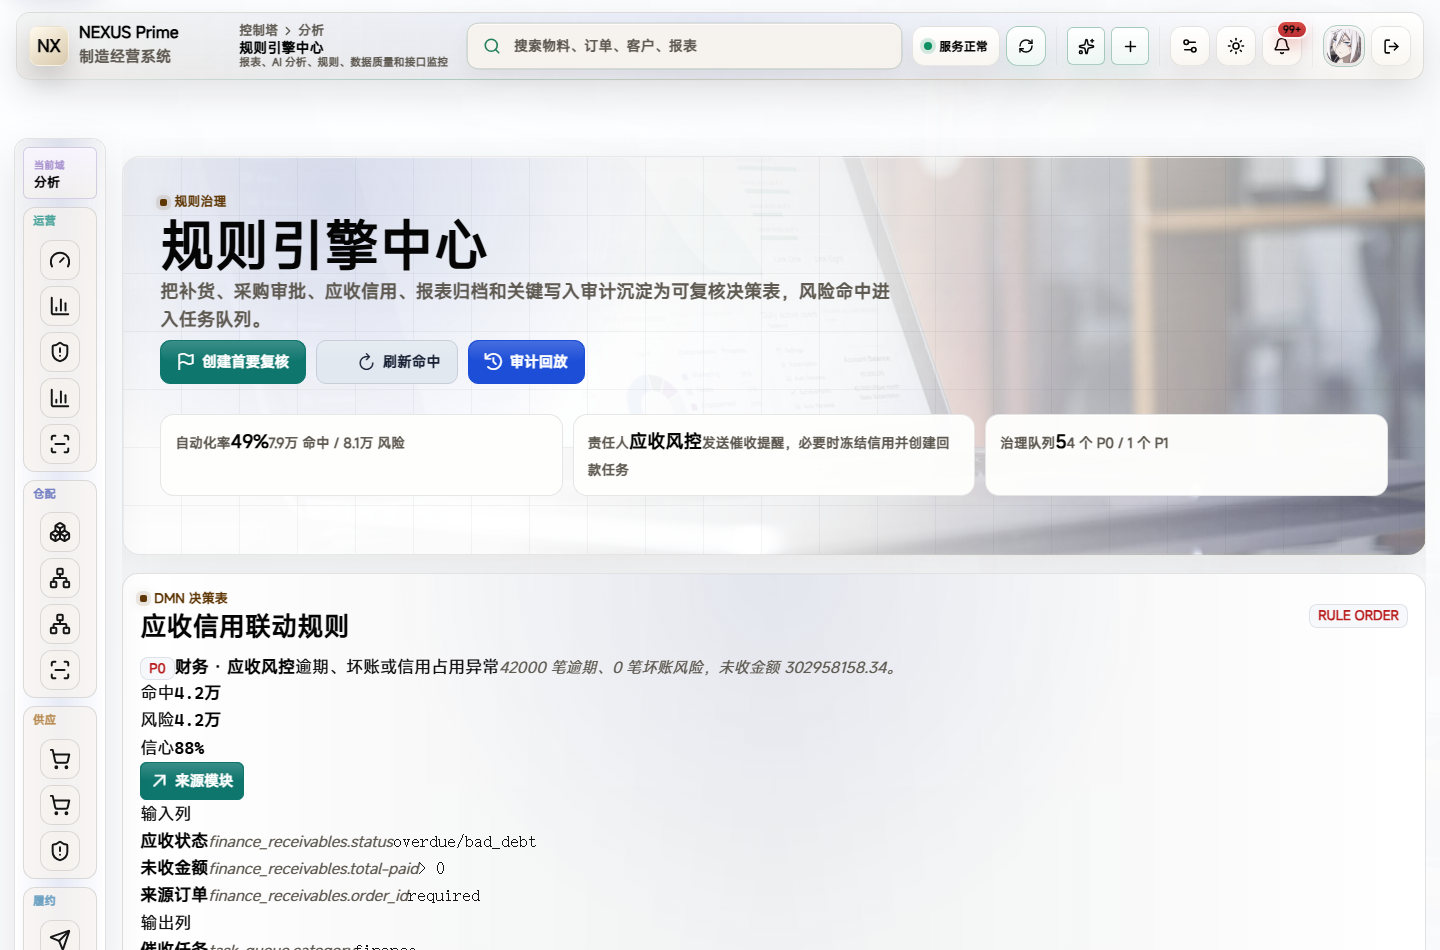
\includegraphics[width=\textwidth,height=0.38\textheight,keepaspectratio]{images/final/pages/desktop-light-luxury-rules.png}
  \caption{规则引擎中心桌面截图，亮色系统}
\end{figure}
\begin{tabularx}{\textwidth}{>{\bfseries}p{0.16\textwidth}X>{\bfseries}p{0.16\textwidth}X}
\toprule
路由 & \code{/app/rules} & 展示主题 & 亮色系统 \\
主要数据 & 规则、通知、报表订阅、补货建议和审计记录。 & 主要接口 & \code{rules, notifications, report-subscriptions} \\
代码关联 & \multicolumn{3}{p{0.7\textwidth}}{\small rules-engine.page.ts + rules/notifications/report-subscriptions} \\
\bottomrule
\end{tabularx}
\vspace{0.5em}
\tightpara{\textbf{页面定位：}规则引擎中心展示预警、审批、补货和报表规则的运行状态。}
\tightpara{\textbf{升级效果：}分析域覆盖报表、规则、数据质量、集成和 AI。它把系统状态、数据可信度和经营建议放到一套分析流程里。本页按照“真实图和关键图表在上、交互报表在中、表单和分页操作台在下”的规则整理，减少无意义跳转方框，让业务动作和数据对象保持同一条线。}
\begin{multicols}{2}
\textbf{主要功能}
\begin{itemize}
  \item 查看规则命中
  \item 管理规则状态
  \item 追踪规则带来的任务和通知
\end{itemize}
\columnbreak
\textbf{验收关注}
\begin{itemize}
  \item 上方区域优先展示真实图、态势图和关键指标，不再堆叠重复入口。
  \item 下方操作台承担搜索、分页、创建、编辑、删除、导出和领域动作。
  \item 页面跳转由 Dock、顶部搜索和资源操作台统一管理，避免随机跳转。
\end{itemize}
\end{multicols}
\clearpage
\subsection{19. 集成监控中心}
\begin{figure}[H]
  \centering
  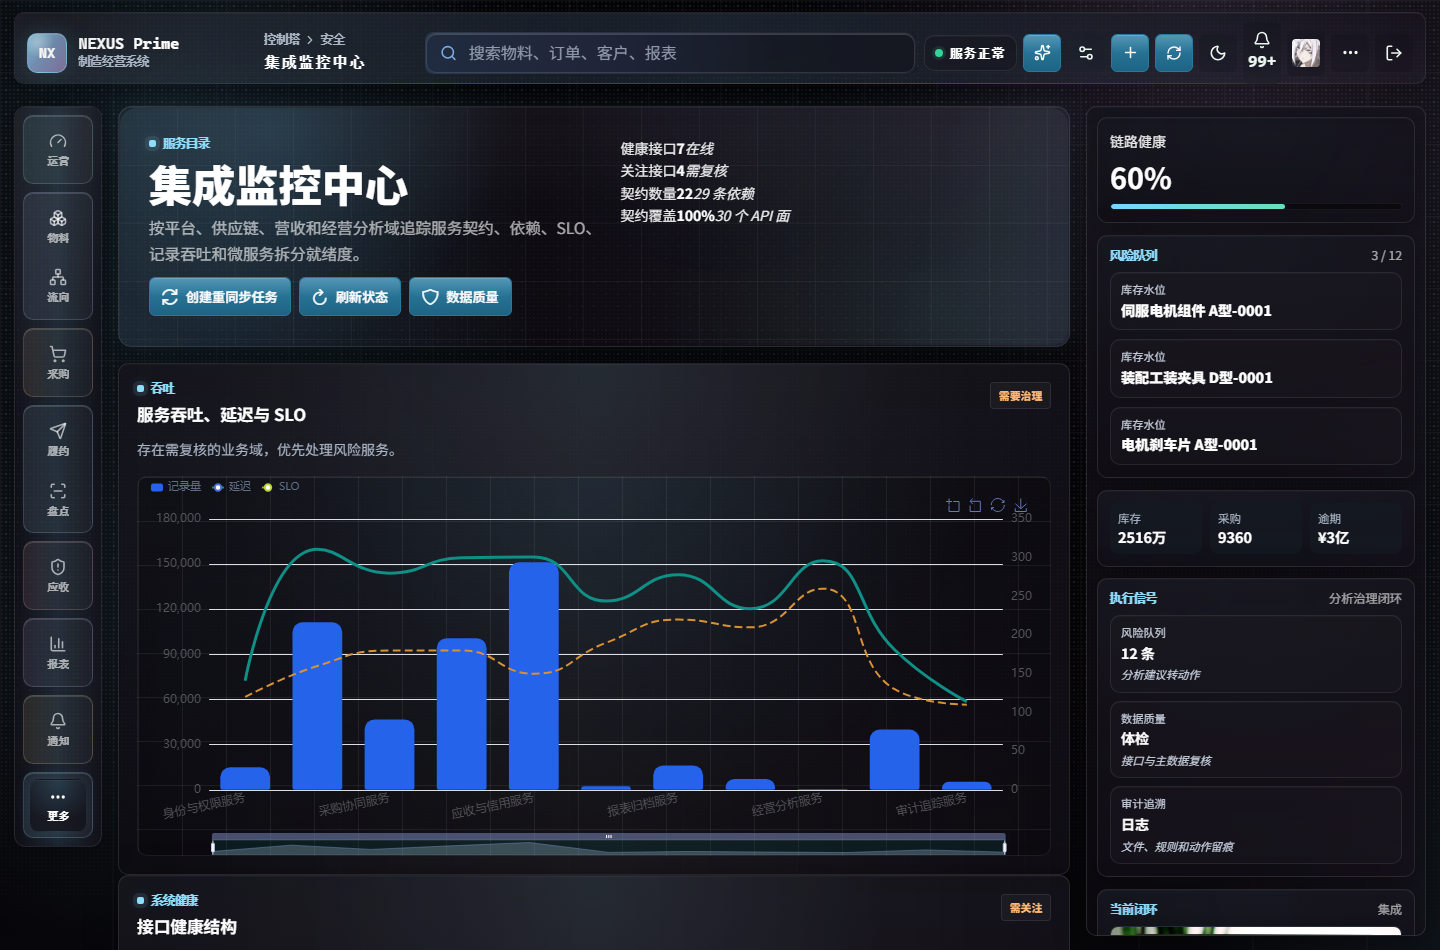
\includegraphics[width=\textwidth,height=0.38\textheight,keepaspectratio]{images/final/pages/desktop-dark-cockpit-integrations.png}
  \caption{集成监控中心桌面截图，深色驾驶舱}
\end{figure}
\begin{tabularx}{\textwidth}{>{\bfseries}p{0.16\textwidth}X>{\bfseries}p{0.16\textwidth}X}
\toprule
路由 & \code{/app/integrations} & 展示主题 & 深色驾驶舱 \\
主要数据 & 后台任务、领域事件、集成状态和错误摘要。 & 主要接口 & \code{integrations, background-jobs, domain-events} \\
代码关联 & \multicolumn{3}{p{0.7\textwidth}}{\small integration-monitor.page.ts + background\_jobs + domain\_events} \\
\bottomrule
\end{tabularx}
\vspace{0.5em}
\tightpara{\textbf{页面定位：}集成监控中心用于查看外部系统、任务队列和数据同步状态。}
\tightpara{\textbf{升级效果：}分析域覆盖报表、规则、数据质量、集成和 AI。它把系统状态、数据可信度和经营建议放到一套分析流程里。本页按照“真实图和关键图表在上、交互报表在中、表单和分页操作台在下”的规则整理，减少无意义跳转方框，让业务动作和数据对象保持同一条线。}
\begin{multicols}{2}
\textbf{主要功能}
\begin{itemize}
  \item 查看集成健康
  \item 识别失败同步
  \item 跟踪后台任务和领域事件
\end{itemize}
\columnbreak
\textbf{验收关注}
\begin{itemize}
  \item 上方区域优先展示真实图、态势图和关键指标，不再堆叠重复入口。
  \item 下方操作台承担搜索、分页、创建、编辑、删除、导出和领域动作。
  \item 页面跳转由 Dock、顶部搜索和资源操作台统一管理，避免随机跳转。
\end{itemize}
\end{multicols}
\clearpage
\subsection{20. 预算成本中心}
\begin{figure}[H]
  \centering
  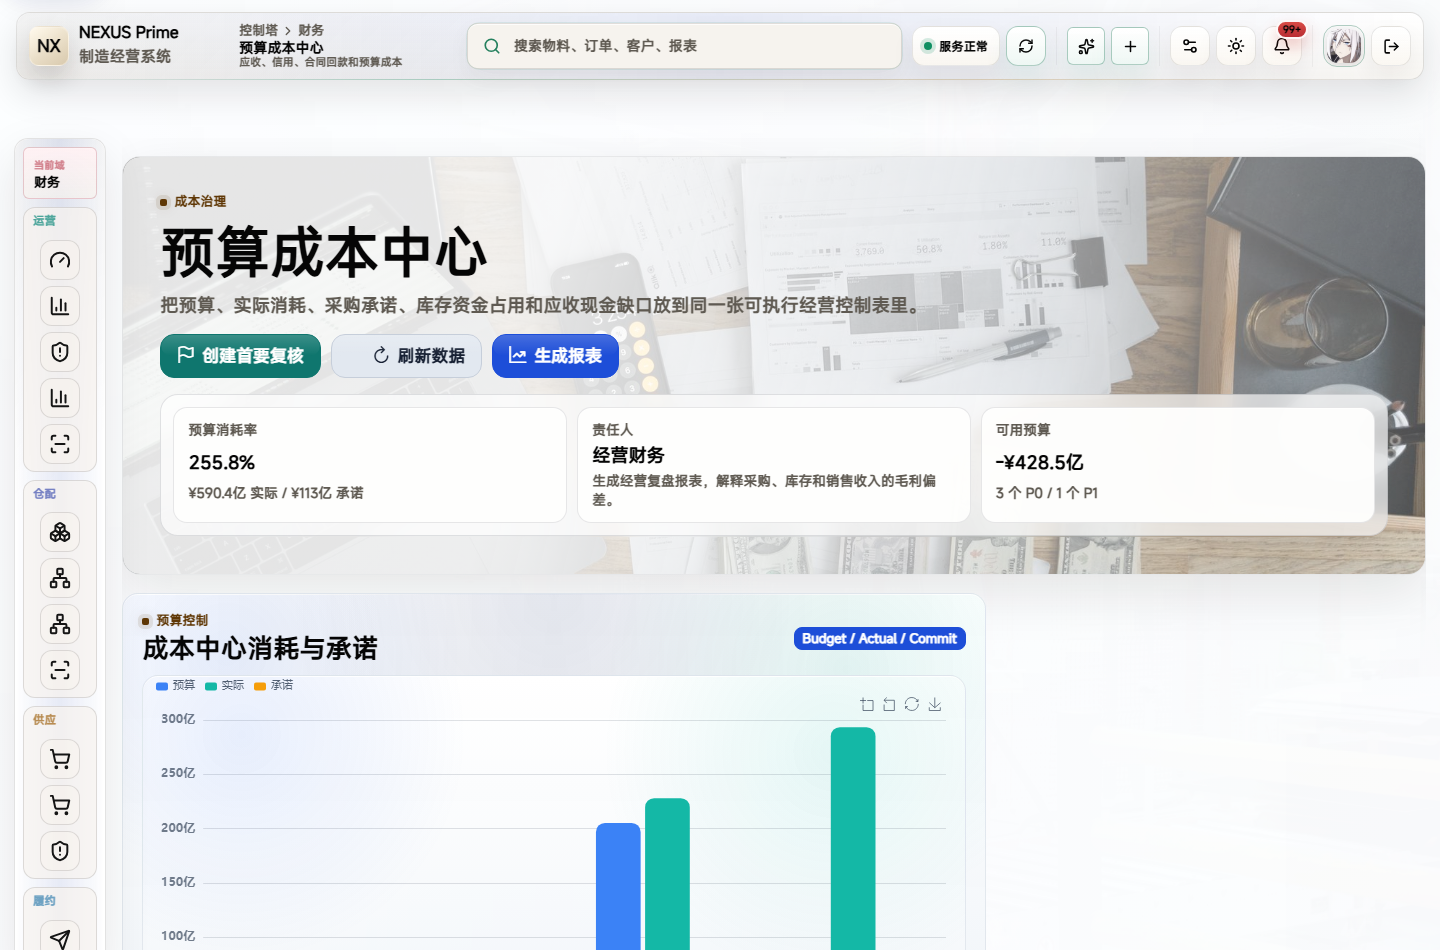
\includegraphics[width=\textwidth,height=0.38\textheight,keepaspectratio]{images/final/pages/desktop-light-luxury-budget.png}
  \caption{预算成本中心桌面截图，亮色系统}
\end{figure}
\begin{tabularx}{\textwidth}{>{\bfseries}p{0.16\textwidth}X>{\bfseries}p{0.16\textwidth}X}
\toprule
路由 & \code{/app/budget} & 展示主题 & 亮色系统 \\
主要数据 & 采购、库存、财务、预算指标和异常任务。 & 主要接口 & \code{operations/costs, operations/costs/review} \\
代码关联 & \multicolumn{3}{p{0.7\textwidth}}{\small budget-cost.page.ts + operations/costs} \\
\bottomrule
\end{tabularx}
\vspace{0.5em}
\tightpara{\textbf{页面定位：}预算成本中心管理采购成本、库存成本、预算偏差和复核动作。}
\tightpara{\textbf{升级效果：}财务域覆盖应收、信用、合同和预算成本。它用账龄、额度、回款和成本偏差表达经营风险，让财务动作能回到订单、客户和合同。本页按照“真实图和关键图表在上、交互报表在中、表单和分页操作台在下”的规则整理，减少无意义跳转方框，让业务动作和数据对象保持同一条线。}
\begin{multicols}{2}
\textbf{主要功能}
\begin{itemize}
  \item 查看预算执行
  \item 识别成本偏差
  \item 发起预算复核
\end{itemize}
\columnbreak
\textbf{验收关注}
\begin{itemize}
  \item 上方区域优先展示真实图、态势图和关键指标，不再堆叠重复入口。
  \item 下方操作台承担搜索、分页、创建、编辑、删除、导出和领域动作。
  \item 页面跳转由 Dock、顶部搜索和资源操作台统一管理，避免随机跳转。
\end{itemize}
\end{multicols}
\clearpage
\subsection{21. 移动扫码终端}
\begin{figure}[H]
  \centering
  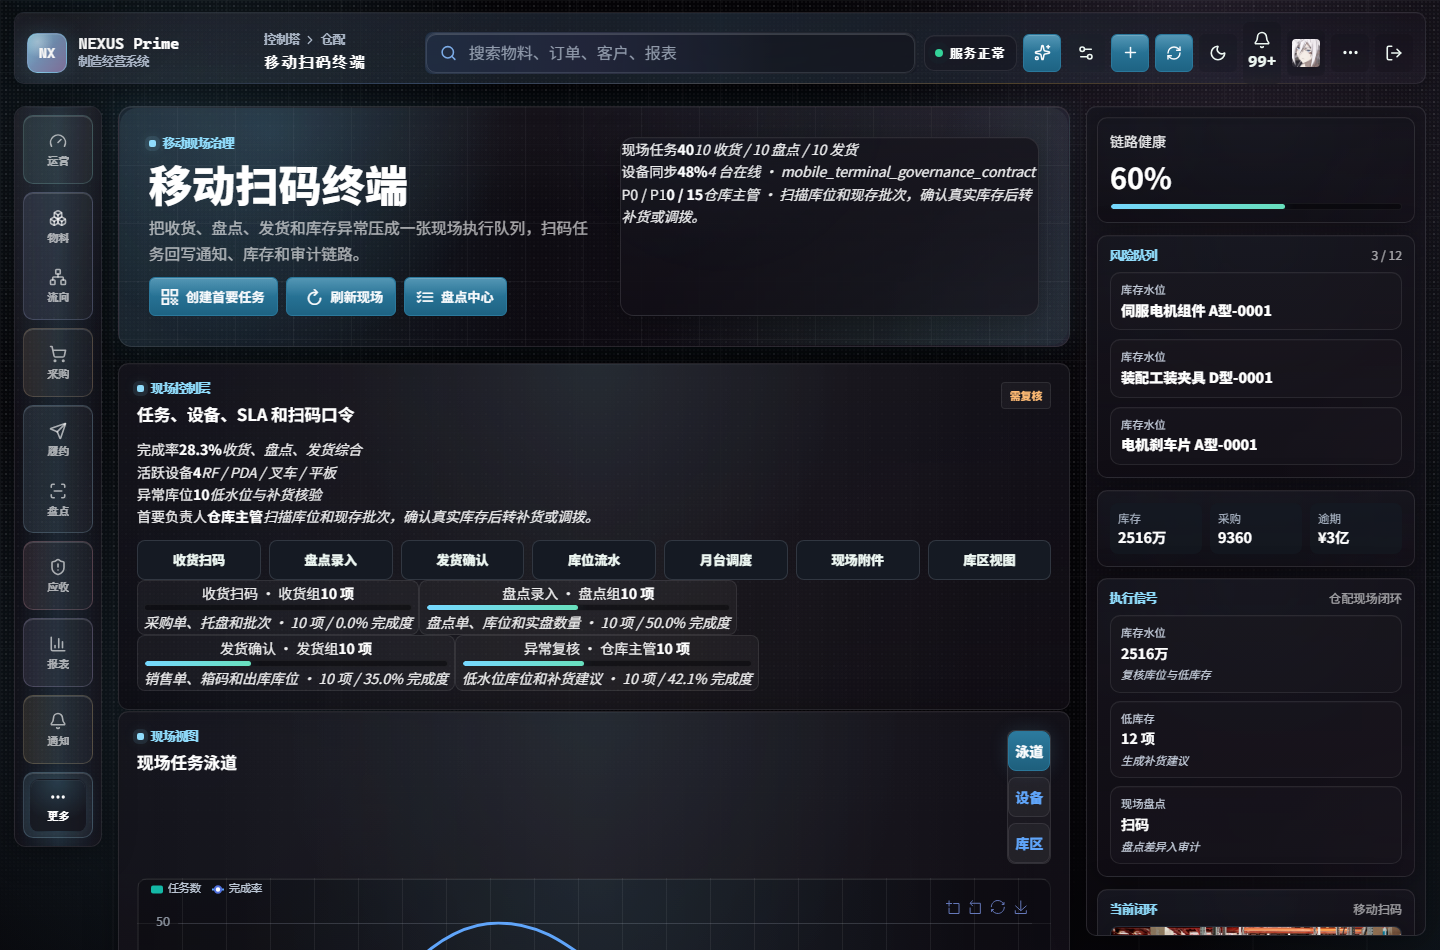
\includegraphics[width=\textwidth,height=0.38\textheight,keepaspectratio]{images/final/pages/desktop-dark-cockpit-mobile-terminal.png}
  \caption{移动扫码终端桌面截图，深色驾驶舱}
\end{figure}
\begin{tabularx}{\textwidth}{>{\bfseries}p{0.16\textwidth}X>{\bfseries}p{0.16\textwidth}X}
\toprule
路由 & \code{/app/mobile-terminal} & 展示主题 & 深色驾驶舱 \\
主要数据 & 移动任务、库存、仓库、盘点和通知。 & 主要接口 & \code{operations/mobile-terminal, operations/mobile-terminal/task} \\
代码关联 & \multicolumn{3}{p{0.7\textwidth}}{\small mobile-terminal.page.ts + operations/mobile-terminal} \\
\bottomrule
\end{tabularx}
\vspace{0.5em}
\tightpara{\textbf{页面定位：}移动扫码终端模拟仓库现场扫码、拣货、上架、盘点和执行记录。}
\tightpara{\textbf{升级效果：}仓配域围绕物料、库存、仓库、库位、扫码和盘点。上方看库存真实场景和流向，中间看交互报表，下方用统一操作台处理库存变动、分页和记录检查。本页按照“真实图和关键图表在上、交互报表在中、表单和分页操作台在下”的规则整理，减少无意义跳转方框，让业务动作和数据对象保持同一条线。}
\begin{multicols}{2}
\textbf{主要功能}
\begin{itemize}
  \item 查看扫码任务
  \item 创建现场任务
  \item 跟踪执行状态和移动端适配
\end{itemize}
\columnbreak
\textbf{验收关注}
\begin{itemize}
  \item 上方区域优先展示真实图、态势图和关键指标，不再堆叠重复入口。
  \item 下方操作台承担搜索、分页、创建、编辑、删除、导出和领域动作。
  \item 页面跳转由 Dock、顶部搜索和资源操作台统一管理，避免随机跳转。
\end{itemize}
\end{multicols}
\clearpage
\subsection{22. 账龄风险墙}
\begin{figure}[H]
  \centering
  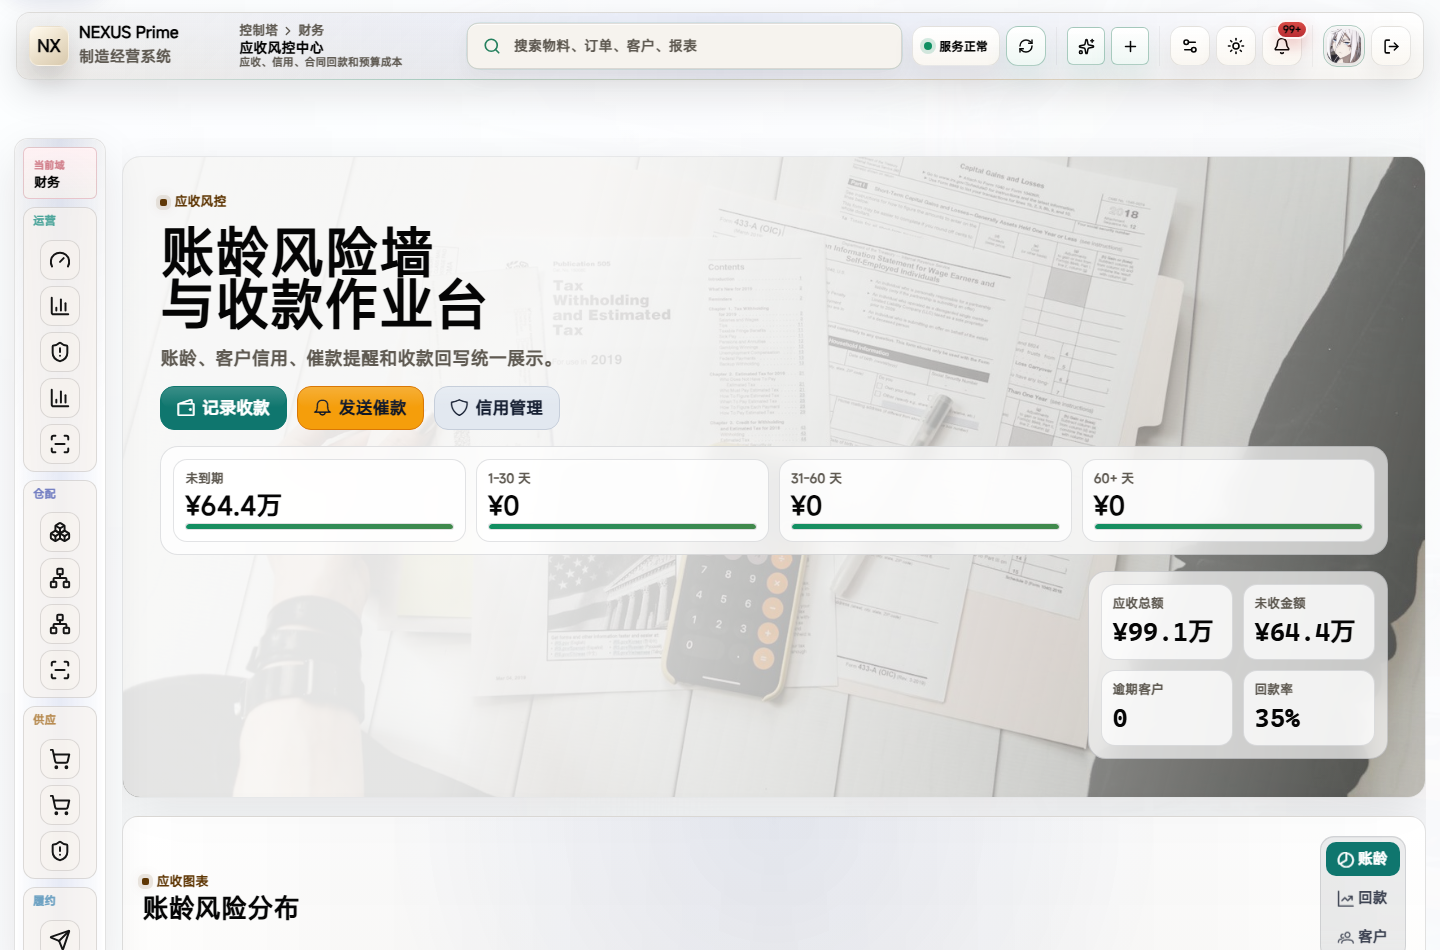
\includegraphics[width=\textwidth,height=0.38\textheight,keepaspectratio]{images/final/pages/desktop-light-luxury-finance-receivables.png}
  \caption{账龄风险墙桌面截图，亮色系统}
\end{figure}
\begin{tabularx}{\textwidth}{>{\bfseries}p{0.16\textwidth}X>{\bfseries}p{0.16\textwidth}X}
\toprule
路由 & \code{/app/finance/receivables} & 展示主题 & 亮色系统 \\
主要数据 & 应收、收款、客户、销售订单和账龄统计。 & 主要接口 & \code{finance/receivables, finance/receivables/aging} \\
代码关联 & \multicolumn{3}{p{0.7\textwidth}}{\small ResourceWorkbench + receivables + payment action} \\
\bottomrule
\end{tabularx}
\vspace{0.5em}
\tightpara{\textbf{页面定位：}账龄风险墙用于查看应收账款、逾期天数、账龄分布和催收动作。}
\tightpara{\textbf{升级效果：}财务域覆盖应收、信用、合同和预算成本。它用账龄、额度、回款和成本偏差表达经营风险，让财务动作能回到订单、客户和合同。本页按照“真实图和关键图表在上、交互报表在中、表单和分页操作台在下”的规则整理，减少无意义跳转方框，让业务动作和数据对象保持同一条线。}
\begin{multicols}{2}
\textbf{主要功能}
\begin{itemize}
  \item 查看应收列表
  \item 登记收款
  \item 分析账龄风险和客户风险
\end{itemize}
\columnbreak
\textbf{验收关注}
\begin{itemize}
  \item 上方区域优先展示真实图、态势图和关键指标，不再堆叠重复入口。
  \item 下方操作台承担搜索、分页、创建、编辑、删除、导出和领域动作。
  \item 页面跳转由 Dock、顶部搜索和资源操作台统一管理，避免随机跳转。
\end{itemize}
\end{multicols}
\clearpage
\subsection{23. 客户信用中心}
\begin{figure}[H]
  \centering
  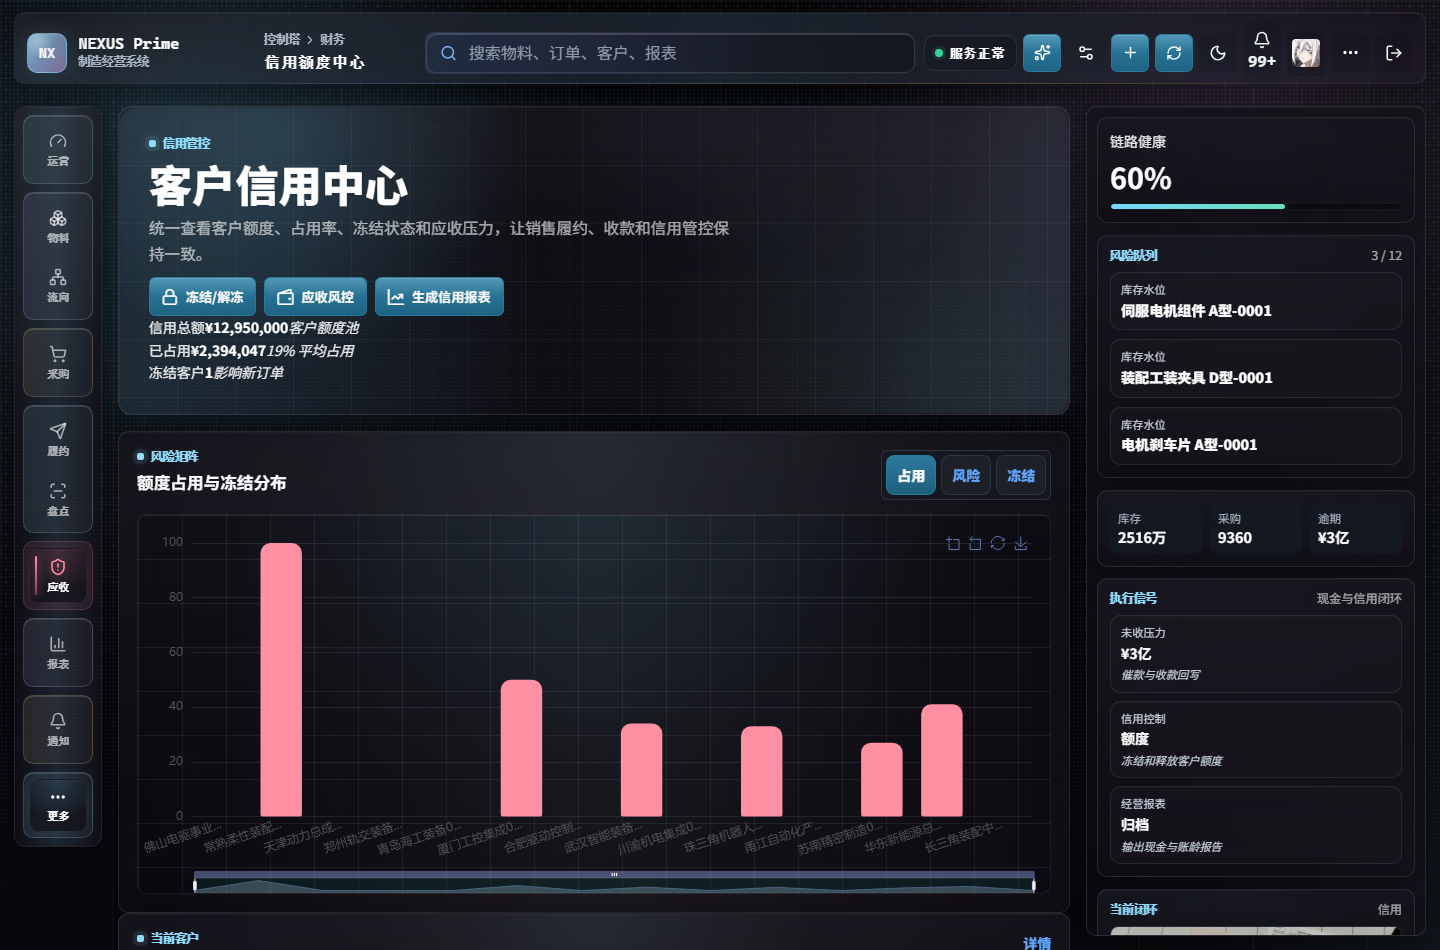
\includegraphics[width=\textwidth,height=0.38\textheight,keepaspectratio]{images/final/pages/desktop-dark-cockpit-finance-credits.png}
  \caption{客户信用中心桌面截图，深色驾驶舱}
\end{figure}
\begin{tabularx}{\textwidth}{>{\bfseries}p{0.16\textwidth}X>{\bfseries}p{0.16\textwidth}X}
\toprule
路由 & \code{/app/finance/credits} & 展示主题 & 深色驾驶舱 \\
主要数据 & 客户信用、客户、订单和应收。 & 主要接口 & \code{finance/credits, finance/credits/:id/freeze} \\
代码关联 & \multicolumn{3}{p{0.7\textwidth}}{\small ResourceWorkbench + credits + freeze/unfreeze action} \\
\bottomrule
\end{tabularx}
\vspace{0.5em}
\tightpara{\textbf{页面定位：}客户信用中心管理信用额度、可用额度、冻结状态和客户风险。}
\tightpara{\textbf{升级效果：}财务域覆盖应收、信用、合同和预算成本。它用账龄、额度、回款和成本偏差表达经营风险，让财务动作能回到订单、客户和合同。本页按照“真实图和关键图表在上、交互报表在中、表单和分页操作台在下”的规则整理，减少无意义跳转方框，让业务动作和数据对象保持同一条线。}
\begin{multicols}{2}
\textbf{主要功能}
\begin{itemize}
  \item 查看客户信用
  \item 冻结或释放信用
  \item 联动订单和应收风险
\end{itemize}
\columnbreak
\textbf{验收关注}
\begin{itemize}
  \item 上方区域优先展示真实图、态势图和关键指标，不再堆叠重复入口。
  \item 下方操作台承担搜索、分页、创建、编辑、删除、导出和领域动作。
  \item 页面跳转由 Dock、顶部搜索和资源操作台统一管理，避免随机跳转。
\end{itemize}
\end{multicols}
\clearpage
\subsection{24. 库存盘点中心}
\begin{figure}[H]
  \centering
  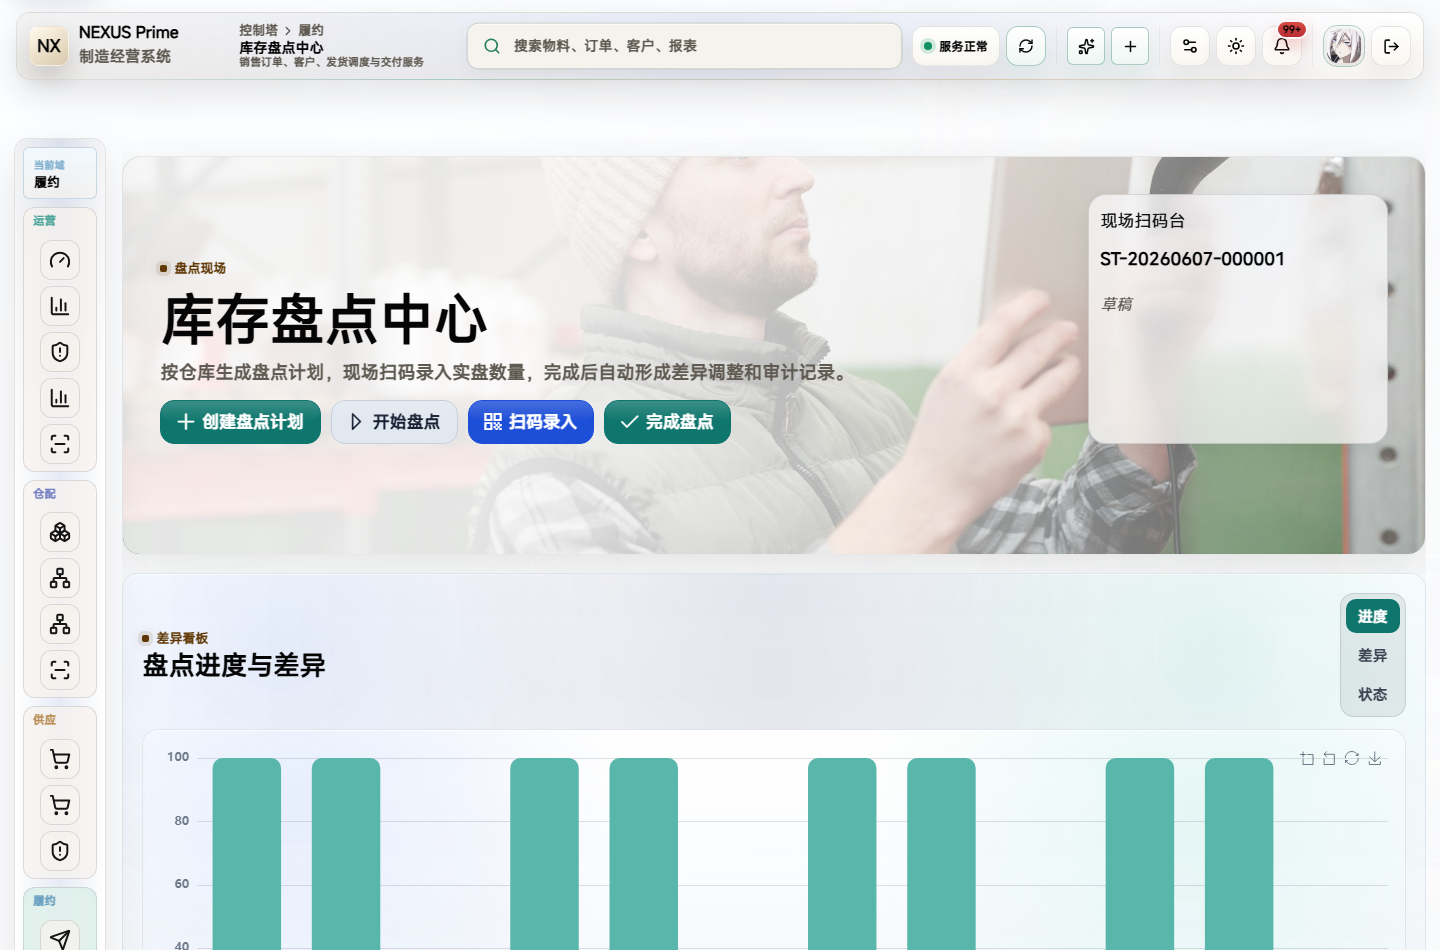
\includegraphics[width=\textwidth,height=0.38\textheight,keepaspectratio]{images/final/pages/desktop-light-luxury-stocktakes.png}
  \caption{库存盘点中心桌面截图，亮色系统}
\end{figure}
\begin{tabularx}{\textwidth}{>{\bfseries}p{0.16\textwidth}X>{\bfseries}p{0.16\textwidth}X}
\toprule
路由 & \code{/app/stocktakes} & 展示主题 & 亮色系统 \\
主要数据 & 盘点单、盘点明细、仓库、商品和库存日志。 & 主要接口 & \code{stocktakes, stocktakes/create, stocktakes/:id/complete} \\
代码关联 & \multicolumn{3}{p{0.7\textwidth}}{\small ResourceWorkbench + stocktakes + stocktake actions} \\
\bottomrule
\end{tabularx}
\vspace{0.5em}
\tightpara{\textbf{页面定位：}库存盘点中心管理盘点单、盘点明细、差异和库存修正。}
\tightpara{\textbf{升级效果：}仓配域围绕物料、库存、仓库、库位、扫码和盘点。上方看库存真实场景和流向，中间看交互报表，下方用统一操作台处理库存变动、分页和记录检查。本页按照“真实图和关键图表在上、交互报表在中、表单和分页操作台在下”的规则整理，减少无意义跳转方框，让业务动作和数据对象保持同一条线。}
\begin{multicols}{2}
\textbf{主要功能}
\begin{itemize}
  \item 创建盘点
  \item 启动和完成盘点
  \item 录入差异并查看调整影响
\end{itemize}
\columnbreak
\textbf{验收关注}
\begin{itemize}
  \item 上方区域优先展示真实图、态势图和关键指标，不再堆叠重复入口。
  \item 下方操作台承担搜索、分页、创建、编辑、删除、导出和领域动作。
  \item 页面跳转由 Dock、顶部搜索和资源操作台统一管理，避免随机跳转。
\end{itemize}
\end{multicols}
\clearpage
\subsection{25. 报表工作室}
\begin{figure}[H]
  \centering
  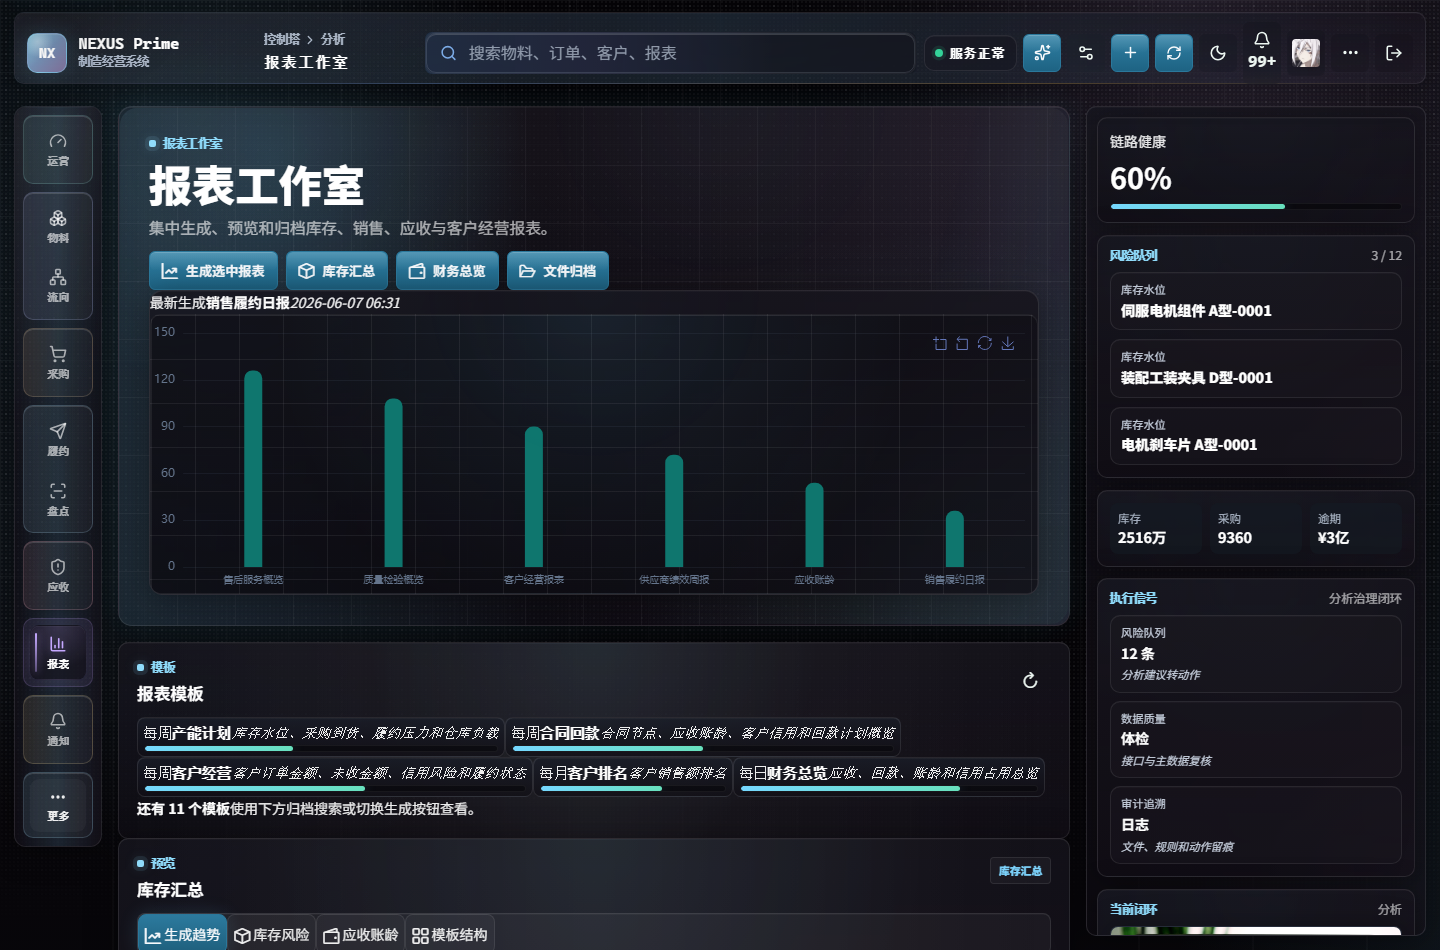
\includegraphics[width=\textwidth,height=0.38\textheight,keepaspectratio]{images/final/pages/desktop-dark-cockpit-reports.png}
  \caption{报表工作室桌面截图，深色驾驶舱}
\end{figure}
\begin{tabularx}{\textwidth}{>{\bfseries}p{0.16\textwidth}X>{\bfseries}p{0.16\textwidth}X}
\toprule
路由 & \code{/app/reports} & 展示主题 & 深色驾驶舱 \\
主要数据 & 生成报表、报表订阅、经营指标和用户。 & 主要接口 & \code{reports/generate, generated-reports, report-subscriptions} \\
代码关联 & \multicolumn{3}{p{0.7\textwidth}}{\small ResourceWorkbench + generated-reports + reports/generate} \\
\bottomrule
\end{tabularx}
\vspace{0.5em}
\tightpara{\textbf{页面定位：}报表工作室用于生成、查看、订阅和下载经营报表。}
\tightpara{\textbf{升级效果：}分析域覆盖报表、规则、数据质量、集成和 AI。它把系统状态、数据可信度和经营建议放到一套分析流程里。本页按照“真实图和关键图表在上、交互报表在中、表单和分页操作台在下”的规则整理，减少无意义跳转方框，让业务动作和数据对象保持同一条线。}
\begin{multicols}{2}
\textbf{主要功能}
\begin{itemize}
  \item 生成报表
  \item 查看报表状态
  \item 管理报表订阅和历史
\end{itemize}
\columnbreak
\textbf{验收关注}
\begin{itemize}
  \item 上方区域优先展示真实图、态势图和关键指标，不再堆叠重复入口。
  \item 下方操作台承担搜索、分页、创建、编辑、删除、导出和领域动作。
  \item 页面跳转由 Dock、顶部搜索和资源操作台统一管理，避免随机跳转。
\end{itemize}
\end{multicols}
\clearpage
\subsection{26. 文件资料库}
\begin{figure}[H]
  \centering
  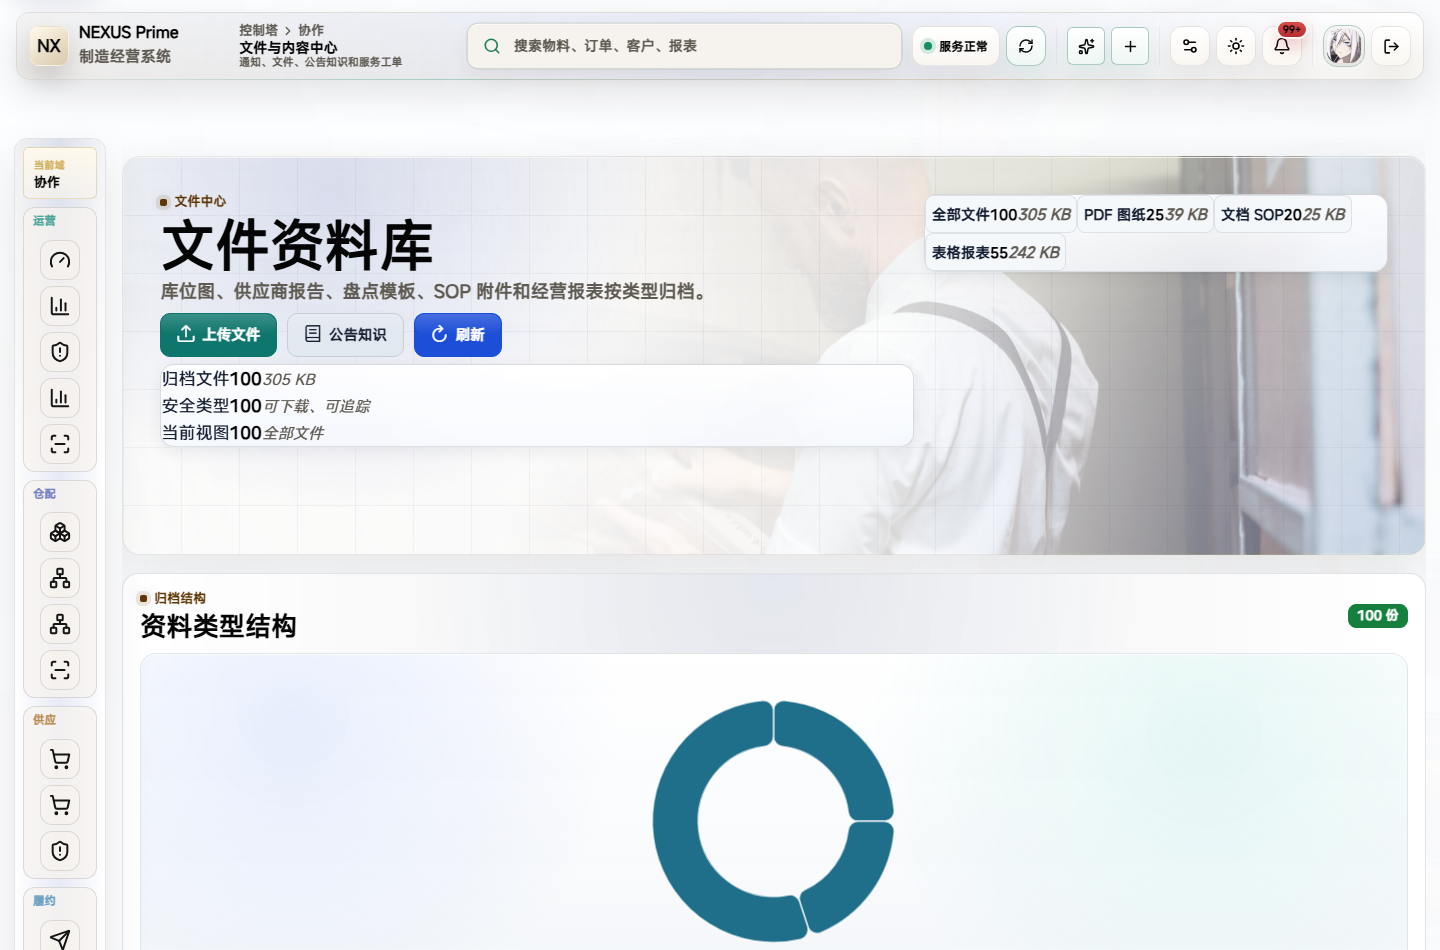
\includegraphics[width=\textwidth,height=0.38\textheight,keepaspectratio]{images/final/pages/desktop-light-luxury-files.png}
  \caption{文件资料库桌面截图，亮色系统}
\end{figure}
\begin{tabularx}{\textwidth}{>{\bfseries}p{0.16\textwidth}X>{\bfseries}p{0.16\textwidth}X}
\toprule
路由 & \code{/app/files} & 展示主题 & 亮色系统 \\
主要数据 & 附件、文章、上传人和业务引用。 & 主要接口 & \code{files/upload, files/:id/download, attachments} \\
代码关联 & \multicolumn{3}{p{0.7\textwidth}}{\small ResourceWorkbench + files/download/upload} \\
\bottomrule
\end{tabularx}
\vspace{0.5em}
\tightpara{\textbf{页面定位：}文件资料库管理业务附件、知识资料、下载和上传。}
\tightpara{\textbf{升级效果：}协作域覆盖通知、文件、公告和服务工单。它让业务结果能形成消息、资料、知识和后续动作，而不是停留在单页操作。本页按照“真实图和关键图表在上、交互报表在中、表单和分页操作台在下”的规则整理，减少无意义跳转方框，让业务动作和数据对象保持同一条线。}
\begin{multicols}{2}
\textbf{主要功能}
\begin{itemize}
  \item 上传文件
  \item 下载附件
  \item 按业务对象查看文件归档
\end{itemize}
\columnbreak
\textbf{验收关注}
\begin{itemize}
  \item 上方区域优先展示真实图、态势图和关键指标，不再堆叠重复入口。
  \item 下方操作台承担搜索、分页、创建、编辑、删除、导出和领域动作。
  \item 页面跳转由 Dock、顶部搜索和资源操作台统一管理，避免随机跳转。
\end{itemize}
\end{multicols}
\clearpage
\subsection{27. 公告与知识库}
\begin{figure}[H]
  \centering
  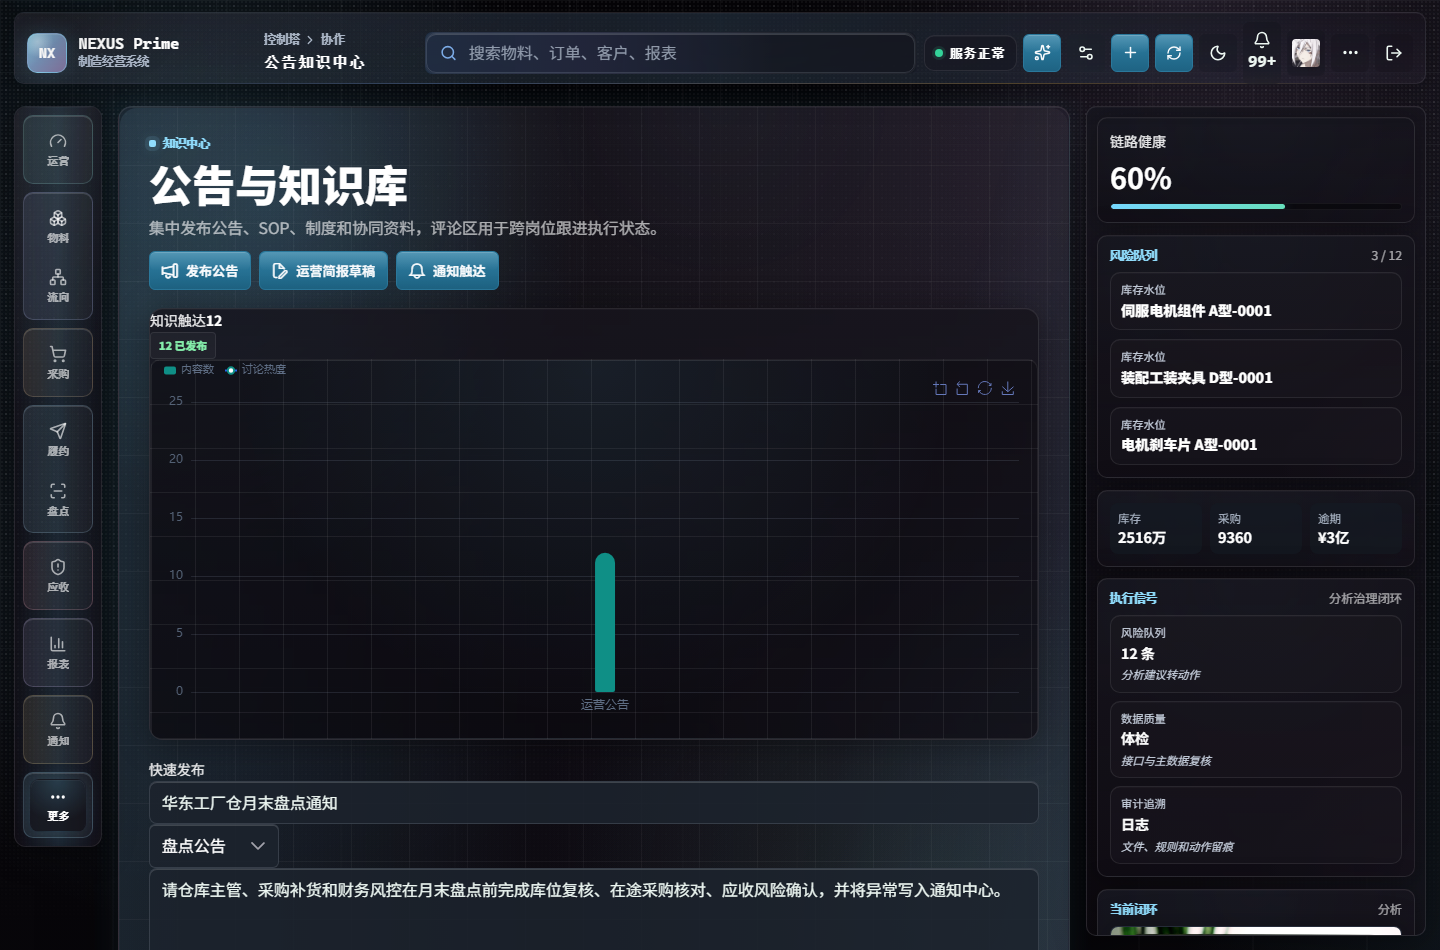
\includegraphics[width=\textwidth,height=0.38\textheight,keepaspectratio]{images/final/pages/desktop-dark-cockpit-content-articles.png}
  \caption{公告与知识库桌面截图，深色驾驶舱}
\end{figure}
\begin{tabularx}{\textwidth}{>{\bfseries}p{0.16\textwidth}X>{\bfseries}p{0.16\textwidth}X}
\toprule
路由 & \code{/app/content/articles} & 展示主题 & 深色驾驶舱 \\
主要数据 & 文章、评论、附件、作者和审计记录。 & 主要接口 & \code{articles, article-comments, attachments} \\
代码关联 & \multicolumn{3}{p{0.7\textwidth}}{\small ResourceWorkbench + articles/comments/attachments} \\
\bottomrule
\end{tabularx}
\vspace{0.5em}
\tightpara{\textbf{页面定位：}公告与知识库发布企业公告、知识文章、评论和附件。}
\tightpara{\textbf{升级效果：}协作域覆盖通知、文件、公告和服务工单。它让业务结果能形成消息、资料、知识和后续动作，而不是停留在单页操作。本页按照“真实图和关键图表在上、交互报表在中、表单和分页操作台在下”的规则整理，减少无意义跳转方框，让业务动作和数据对象保持同一条线。}
\begin{multicols}{2}
\textbf{主要功能}
\begin{itemize}
  \item 查看文章
  \item 维护公告
  \item 评论和引用附件
\end{itemize}
\columnbreak
\textbf{验收关注}
\begin{itemize}
  \item 上方区域优先展示真实图、态势图和关键指标，不再堆叠重复入口。
  \item 下方操作台承担搜索、分页、创建、编辑、删除、导出和领域动作。
  \item 页面跳转由 Dock、顶部搜索和资源操作台统一管理，避免随机跳转。
\end{itemize}
\end{multicols}
\clearpage
\subsection{28. 系统安全中心}
\begin{figure}[H]
  \centering
  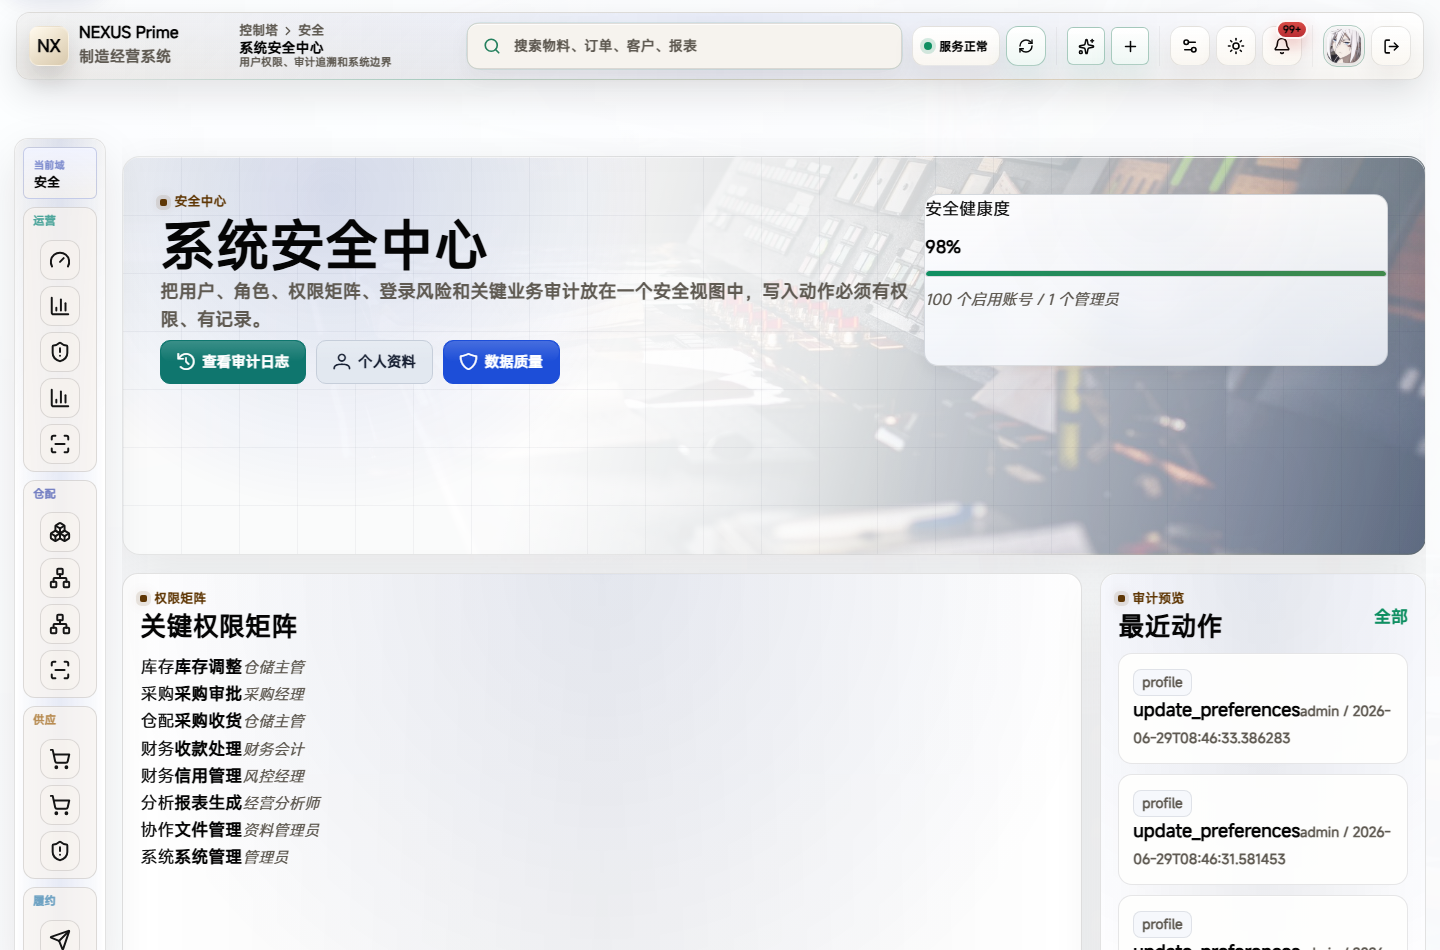
\includegraphics[width=\textwidth,height=0.38\textheight,keepaspectratio]{images/final/pages/desktop-light-luxury-system-users.png}
  \caption{系统安全中心桌面截图，亮色系统}
\end{figure}
\begin{tabularx}{\textwidth}{>{\bfseries}p{0.16\textwidth}X>{\bfseries}p{0.16\textwidth}X}
\toprule
路由 & \code{/app/system/users} & 展示主题 & 亮色系统 \\
主要数据 & 用户、角色、权限、部门和审计。 & 主要接口 & \code{users, roles, permissions, departments} \\
代码关联 & \multicolumn{3}{p{0.7\textwidth}}{\small ResourceWorkbench + users/roles/permissions} \\
\bottomrule
\end{tabularx}
\vspace{0.5em}
\tightpara{\textbf{页面定位：}系统安全中心管理账号、角色、部门、权限和账号状态。}
\tightpara{\textbf{升级效果：}安全域覆盖用户、权限、审计和集成边界。核心是让谁做了什么、能做什么、何时做的都有清晰证据。本页按照“真实图和关键图表在上、交互报表在中、表单和分页操作台在下”的规则整理，减少无意义跳转方框，让业务动作和数据对象保持同一条线。}
\begin{multicols}{2}
\textbf{主要功能}
\begin{itemize}
  \item 查看用户列表
  \item 调整角色和账号状态
  \item 检查权限边界
\end{itemize}
\columnbreak
\textbf{验收关注}
\begin{itemize}
  \item 上方区域优先展示真实图、态势图和关键指标，不再堆叠重复入口。
  \item 下方操作台承担搜索、分页、创建、编辑、删除、导出和领域动作。
  \item 页面跳转由 Dock、顶部搜索和资源操作台统一管理，避免随机跳转。
\end{itemize}
\end{multicols}
\clearpage
\subsection{29. 审计日志}
\begin{figure}[H]
  \centering
  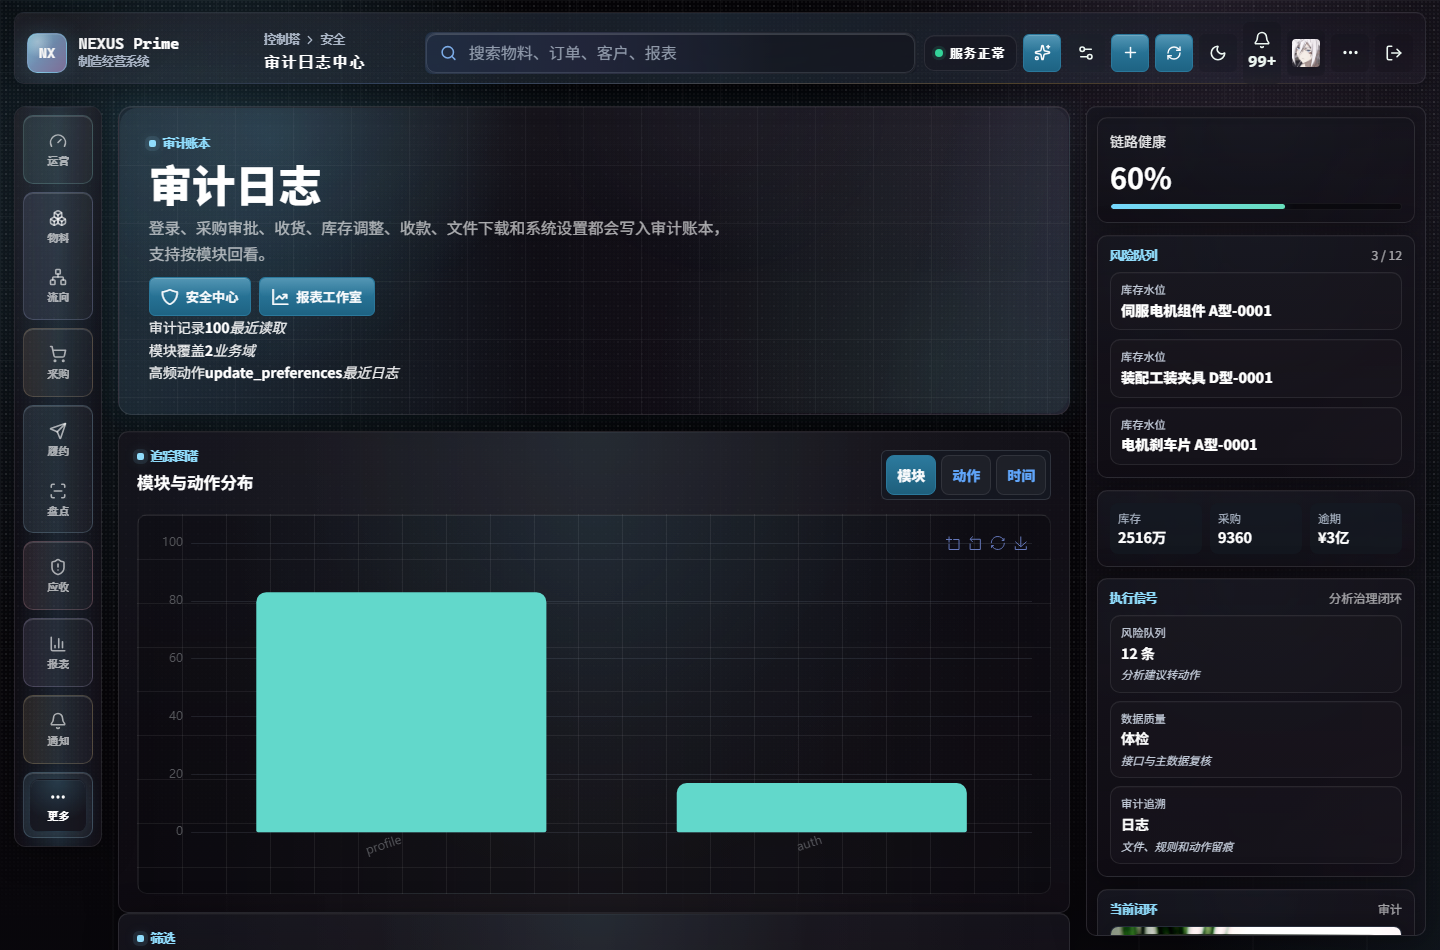
\includegraphics[width=\textwidth,height=0.38\textheight,keepaspectratio]{images/final/pages/desktop-dark-cockpit-system-audit.png}
  \caption{审计日志桌面截图，深色驾驶舱}
\end{figure}
\begin{tabularx}{\textwidth}{>{\bfseries}p{0.16\textwidth}X>{\bfseries}p{0.16\textwidth}X}
\toprule
路由 & \code{/app/system/audit} & 展示主题 & 深色驾驶舱 \\
主要数据 & 审计日志、用户、模块、动作和请求上下文。 & 主要接口 & \code{audit-logs} \\
代码关联 & \multicolumn{3}{p{0.7\textwidth}}{\small ResourceWorkbench + audit-logs} \\
\bottomrule
\end{tabularx}
\vspace{0.5em}
\tightpara{\textbf{页面定位：}审计日志页面集中展示登录、写入、审批、删除和系统动作留痕。}
\tightpara{\textbf{升级效果：}安全域覆盖用户、权限、审计和集成边界。核心是让谁做了什么、能做什么、何时做的都有清晰证据。本页按照“真实图和关键图表在上、交互报表在中、表单和分页操作台在下”的规则整理，减少无意义跳转方框，让业务动作和数据对象保持同一条线。}
\begin{multicols}{2}
\textbf{主要功能}
\begin{itemize}
  \item 查看审计日志
  \item 按用户和动作追踪
  \item 支撑问题回溯和课程验收
\end{itemize}
\columnbreak
\textbf{验收关注}
\begin{itemize}
  \item 上方区域优先展示真实图、态势图和关键指标，不再堆叠重复入口。
  \item 下方操作台承担搜索、分页、创建、编辑、删除、导出和领域动作。
  \item 页面跳转由 Dock、顶部搜索和资源操作台统一管理，避免随机跳转。
\end{itemize}
\end{multicols}
\clearpage
\subsection{30. 任务通知中心}
\begin{figure}[H]
  \centering
  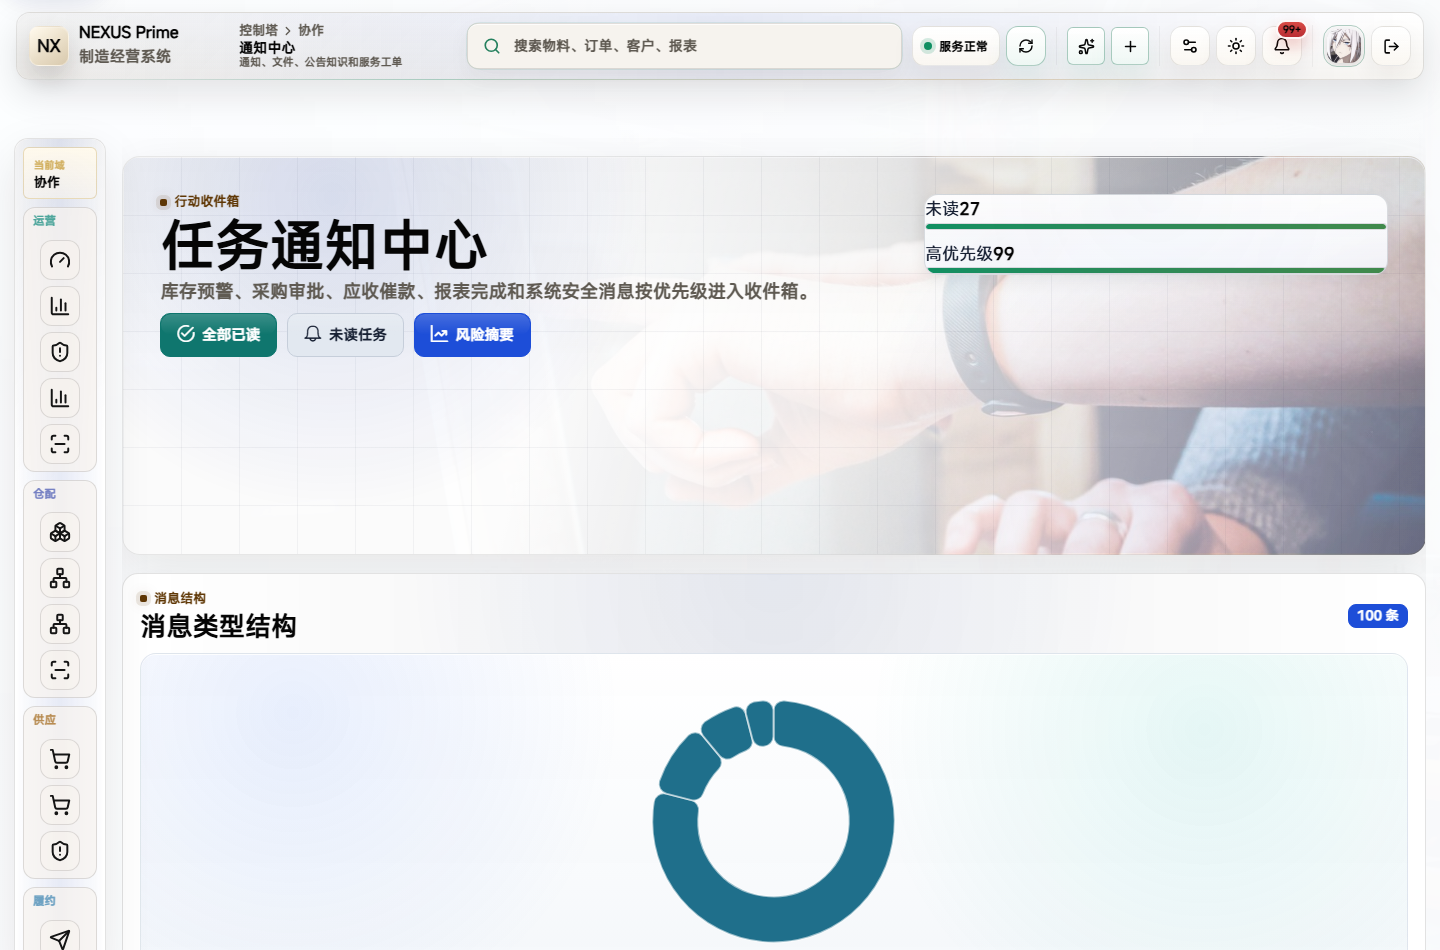
\includegraphics[width=\textwidth,height=0.38\textheight,keepaspectratio]{images/final/pages/desktop-light-luxury-notifications.png}
  \caption{任务通知中心桌面截图，亮色系统}
\end{figure}
\begin{tabularx}{\textwidth}{>{\bfseries}p{0.16\textwidth}X>{\bfseries}p{0.16\textwidth}X}
\toprule
路由 & \code{/app/notifications} & 展示主题 & 亮色系统 \\
主要数据 & 系统通知、库存预警、任务事件和用户。 & 主要接口 & \code{notifications, notifications/mark-read} \\
代码关联 & \multicolumn{3}{p{0.7\textwidth}}{\small ResourceWorkbench + notifications/mark-read} \\
\bottomrule
\end{tabularx}
\vspace{0.5em}
\tightpara{\textbf{页面定位：}任务通知中心用于查看未读、已读、异常和业务提醒。}
\tightpara{\textbf{升级效果：}协作域覆盖通知、文件、公告和服务工单。它让业务结果能形成消息、资料、知识和后续动作，而不是停留在单页操作。本页按照“真实图和关键图表在上、交互报表在中、表单和分页操作台在下”的规则整理，减少无意义跳转方框，让业务动作和数据对象保持同一条线。}
\begin{multicols}{2}
\textbf{主要功能}
\begin{itemize}
  \item 查看通知
  \item 标记已读
  \item 从通知进入业务对象
\end{itemize}
\columnbreak
\textbf{验收关注}
\begin{itemize}
  \item 上方区域优先展示真实图、态势图和关键指标，不再堆叠重复入口。
  \item 下方操作台承担搜索、分页、创建、编辑、删除、导出和领域动作。
  \item 页面跳转由 Dock、顶部搜索和资源操作台统一管理，避免随机跳转。
\end{itemize}
\end{multicols}
\clearpage
\subsection{31. 经营分析台}
\begin{figure}[H]
  \centering
  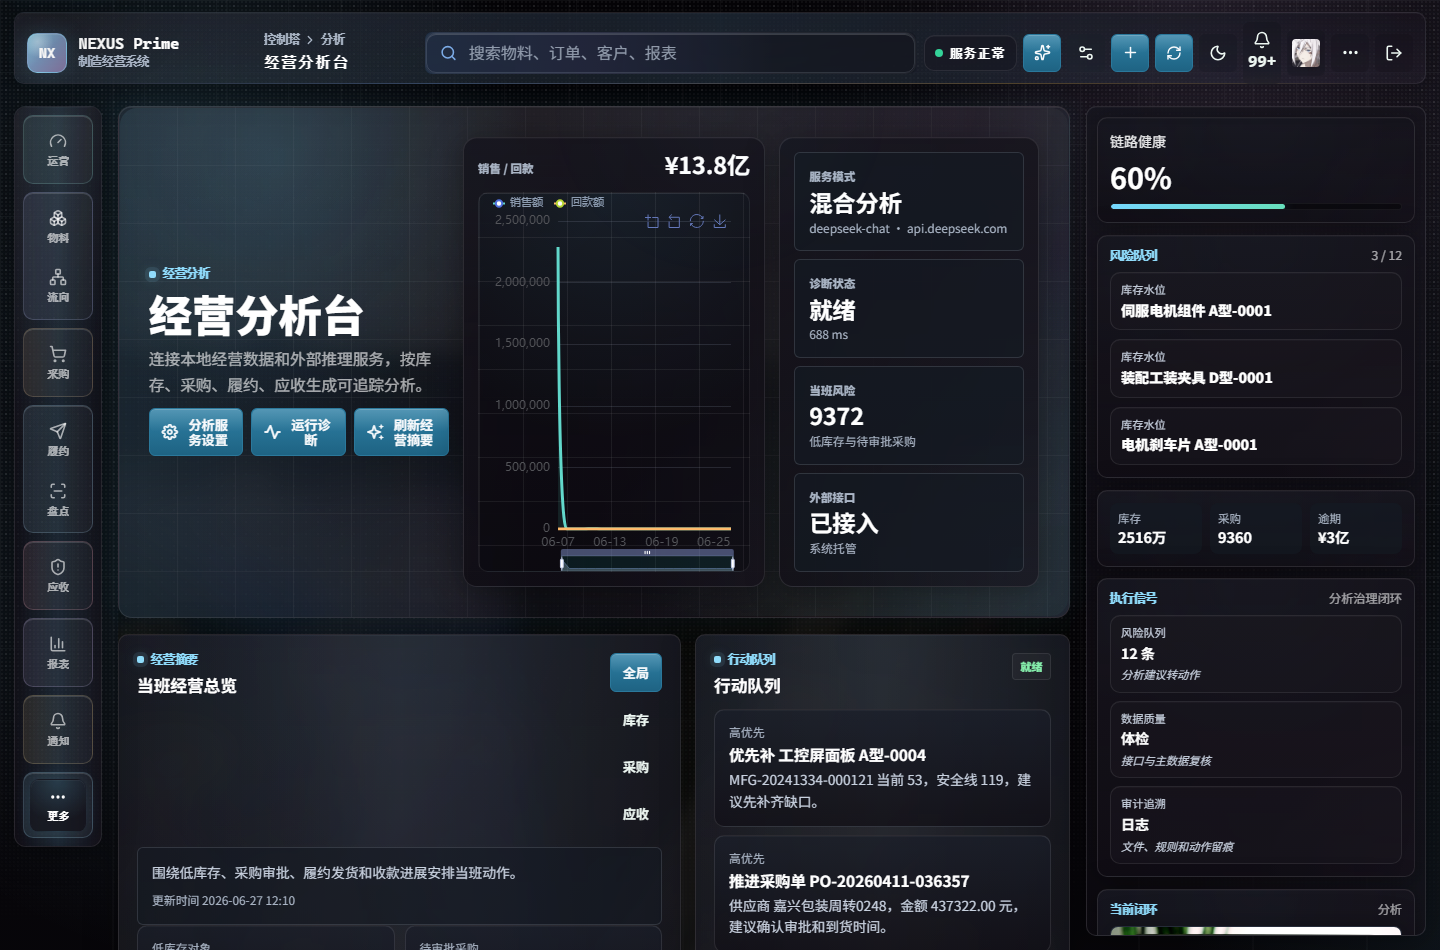
\includegraphics[width=\textwidth,height=0.38\textheight,keepaspectratio]{images/final/pages/desktop-dark-cockpit-ai.png}
  \caption{经营分析台桌面截图，深色驾驶舱}
\end{figure}
\begin{tabularx}{\textwidth}{>{\bfseries}p{0.16\textwidth}X>{\bfseries}p{0.16\textwidth}X}
\toprule
路由 & \code{/app/ai} & 展示主题 & 深色驾驶舱 \\
主要数据 & AI 会话、消息、经营指标、文档分块和动作草稿。 & 主要接口 & \code{ai/chat, ai/analyze/structured, ai/diagnostics} \\
代码关联 & \multicolumn{3}{p{0.7\textwidth}}{\small ResourceWorkbench + ai/chat + ai/analyze/structured} \\
\bottomrule
\end{tabularx}
\vspace{0.5em}
\tightpara{\textbf{页面定位：}经营分析台提供 AI 对话、结构化诊断、经营建议和动作草稿。}
\tightpara{\textbf{升级效果：}分析域覆盖报表、规则、数据质量、集成和 AI。它把系统状态、数据可信度和经营建议放到一套分析流程里。本页按照“真实图和关键图表在上、交互报表在中、表单和分页操作台在下”的规则整理，减少无意义跳转方框，让业务动作和数据对象保持同一条线。}
\begin{multicols}{2}
\textbf{主要功能}
\begin{itemize}
  \item 发起经营问答
  \item 生成结构化分析
  \item 查看 AI 会话和动作草稿
\end{itemize}
\columnbreak
\textbf{验收关注}
\begin{itemize}
  \item 上方区域优先展示真实图、态势图和关键指标，不再堆叠重复入口。
  \item 下方操作台承担搜索、分页、创建、编辑、删除、导出和领域动作。
  \item 页面跳转由 Dock、顶部搜索和资源操作台统一管理，避免随机跳转。
\end{itemize}
\end{multicols}
\clearpage
\subsection{32. 个人中心}
\begin{figure}[H]
  \centering
  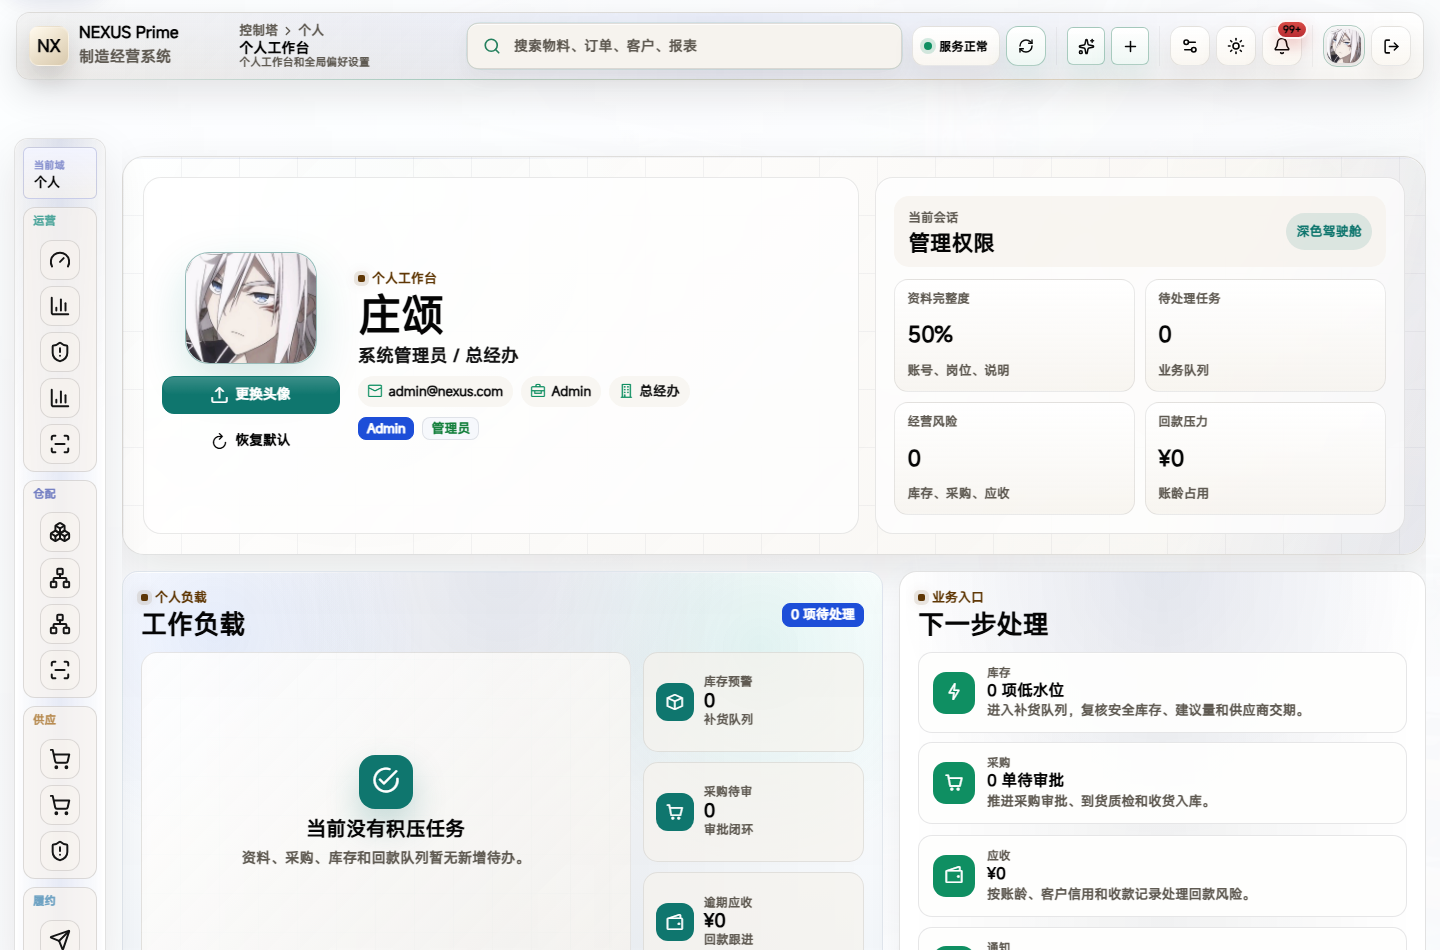
\includegraphics[width=\textwidth,height=0.38\textheight,keepaspectratio]{images/final/pages/desktop-light-luxury-profile.png}
  \caption{个人中心桌面截图，亮色系统}
\end{figure}
\begin{tabularx}{\textwidth}{>{\bfseries}p{0.16\textwidth}X>{\bfseries}p{0.16\textwidth}X}
\toprule
路由 & \code{/app/profile} & 展示主题 & 亮色系统 \\
主要数据 & 当前用户、头像、偏好、通知和待办。 & 主要接口 & \code{me/profile, me/avatar, me/preferences, operations/todo} \\
代码关联 & \multicolumn{3}{p{0.7\textwidth}}{\small profile.page.ts + me/profile + me/preferences} \\
\bottomrule
\end{tabularx}
\vspace{0.5em}
\tightpara{\textbf{页面定位：}个人中心管理身份资料、头像、偏好、工作负载和最近业务入口。}
\tightpara{\textbf{升级效果：}个人域覆盖个人资料、头像、偏好、默认工作台和控制中心。它把用户自己的工作环境整理为可维护的独立区域。本页按照“真实图和关键图表在上、交互报表在中、表单和分页操作台在下”的规则整理，减少无意义跳转方框，让业务动作和数据对象保持同一条线。}
\begin{multicols}{2}
\textbf{主要功能}
\begin{itemize}
  \item 更新个人资料
  \item 上传或恢复头像
  \item 查看个人待办和偏好
\end{itemize}
\columnbreak
\textbf{验收关注}
\begin{itemize}
  \item 上方区域优先展示真实图、态势图和关键指标，不再堆叠重复入口。
  \item 下方操作台承担搜索、分页、创建、编辑、删除、导出和领域动作。
  \item 页面跳转由 Dock、顶部搜索和资源操作台统一管理，避免随机跳转。
\end{itemize}
\end{multicols}
\clearpage
\subsection{33. 控制中心}
\begin{figure}[H]
  \centering
  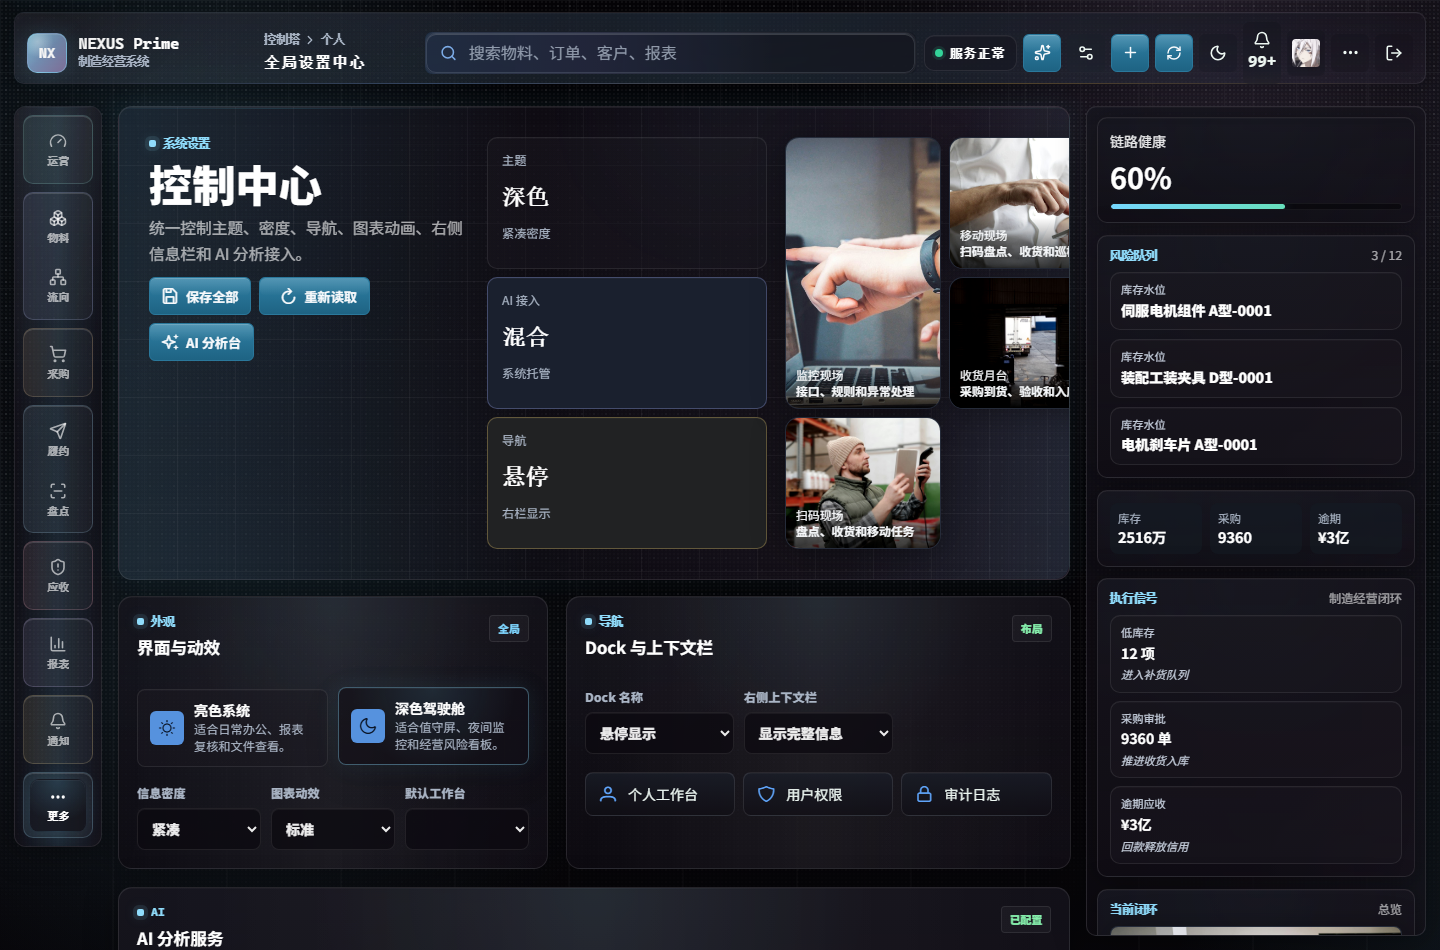
\includegraphics[width=\textwidth,height=0.38\textheight,keepaspectratio]{images/final/pages/desktop-dark-cockpit-settings.png}
  \caption{控制中心桌面截图，深色驾驶舱}
\end{figure}
\begin{tabularx}{\textwidth}{>{\bfseries}p{0.16\textwidth}X>{\bfseries}p{0.16\textwidth}X}
\toprule
路由 & \code{/app/settings} & 展示主题 & 深色驾驶舱 \\
主要数据 & 个人偏好、健康检查、AI 状态和系统配置摘要。 & 主要接口 & \code{me/preferences, health, observability/metrics} \\
代码关联 & \multicolumn{3}{p{0.7\textwidth}}{\small settings.page.ts + health + preferences + theme} \\
\bottomrule
\end{tabularx}
\vspace{0.5em}
\tightpara{\textbf{页面定位：}控制中心管理主题、密度、部署状态、AI 配置提示和系统能力概览。}
\tightpara{\textbf{升级效果：}个人域覆盖个人资料、头像、偏好、默认工作台和控制中心。它把用户自己的工作环境整理为可维护的独立区域。本页按照“真实图和关键图表在上、交互报表在中、表单和分页操作台在下”的规则整理，减少无意义跳转方框，让业务动作和数据对象保持同一条线。}
\begin{multicols}{2}
\textbf{主要功能}
\begin{itemize}
  \item 查看运行配置
  \item 调整主题偏好
  \item 检查部署就绪和系统能力
\end{itemize}
\columnbreak
\textbf{验收关注}
\begin{itemize}
  \item 上方区域优先展示真实图、态势图和关键指标，不再堆叠重复入口。
  \item 下方操作台承担搜索、分页、创建、编辑、删除、导出和领域动作。
  \item 页面跳转由 Dock、顶部搜索和资源操作台统一管理，避免随机跳转。
\end{itemize}
\end{multicols}
\clearpage
\section{核心代码详解}
\subsection{前端 API 和会话}
\code{frontend/src/app/core/api.service.ts} 统一封装 \code{HttpClient}。所有请求带 \code{withCredentials: true}，浏览器自动携带 HttpOnly Cookie，页面只关心业务数据。返回值通过 envelope 解包，减少重复样板代码。查询参数统一过滤空值，列表页、搜索页和资源操作台不用重复判断 \code{undefined}、\code{null} 和空字符串。

\code{frontend/src/app/core/auth.service.ts} 保存当前用户和权限摘要，登录后写入 CSRF token，刷新后通过 \code{auth.guard.ts} 保护 \code{/app/**}。如果 Cookie 仍有效，会调用 \code{/auth/me} 恢复会话；没有登录态才跳回登录页。\code{auth.interceptor.ts} 对写操作附加 \code{X-CSRF-Token}，并把 401、403、500 等错误统一转成页面消息。

\subsection{Shell、Dock 和顶部导航}
\code{app-shell.component.ts} 承担登录后壳层职责，包括搜索防抖、通知轮询、服务健康、模块状态、路由 loading、页面滚动复位和页面容器。\code{navigation.ts} 把所有 \code{/app/**} 路由映射到统一 Dock 分组、当前项、兄弟项和面包屑。\code{app-dock.component.ts} 是左侧核心流程入口，按钮不再拉长，只保留稳定图标、当前状态、短标签和文字浮窗。\code{app-topbar.component.ts} 合并搜索、面包屑、服务状态、快捷创建、AI、主题按钮、通知、头像和退出。

\subsection{资源操作台}
\code{resource-workflow.ts} 把物料、仓配、补货、采购、销售、客户、应收、信用、盘点、报表、文件、内容、通知、用户、审计和 AI 会话配置为资源工作流。每个资源定义字段、列、搜索、创建端点、更新端点、领域动作和导出能力。\code{resource-workbench.component.ts} 根据当前 URL 自动选择配置，统一渲染搜索、分页、记录列表、详情检查、创建表单、编辑表单、删除确认和动作执行。这是下半部分 CRUD 排版统一的关键。

\subsection{后端认证、策略和 CRUD}
\code{backend/app/api/auth_routes.py} 负责登录、注册、退出、CSRF、当前用户和修改密码。\code{backend/app/platform/auth/decorators.py} 提供 \code{jwt_required}、\code{csrf_required} 和 \code{permission_required}。\code{backend/app/platform/policy/policy_engine.py} 集中处理管理员、权限集合、资源权限、对象授权和字段过滤。\code{generic_crud_routes.py} 通过资源注册表复用分页、搜索、创建、更新、删除、权限和审计逻辑。这样前端资源操作台能够通过统一 API 访问不同业务对象。

\subsection{完整数据库启动}
\code{backend/scripts/bootstrap_sqlite.py} 是本次完整数据上线的关键。它会读取 \code{backend/.env}，下载 \code{.db.gz} 文件，解压到 \code{/tmp/nexus-prime/nexus_prime.db}，执行写锁测试、\code{pragma quick_check}，并确认用户数和销售订单数达到阈值。这样可以防止空库误上线。脚本还会在已有数据库足够大且未强制刷新时复用现有文件，避免每次启动都重复下载 46MB 压缩库。

\subsection{代码链路验收点}
\begin{longtable}{p{0.24\textwidth}p{0.66\textwidth}}
\toprule
链路 & 验收重点 \\
\midrule
\endhead
入口保护 & 首页、登录页、注册页不改源码，只通过主题偏好截图；登录后才进入 \code{/app/**}。 \\
会话恢复 & Cookie 存在时 \code{authGuard} 调用 \code{/auth/me} 恢复用户，避免刷新后误跳登录。 \\
全局请求 & \code{ApiService} 和 interceptor 统一凭据、CSRF、错误提示和 envelope 解包。 \\
导航归一 & \code{navigation.ts} 是 Dock、面包屑、当前模块和跳转规则的唯一业务地图。 \\
主题切换 & \code{ThemeService} 只暴露深色与亮色两个实际状态，并广播图表刷新事件。 \\
资源操作 & \code{ResourceWorkbench} 统一搜索、分页、表单、动作、导出和审计提示。 \\
后端边界 & 权限装饰器和策略引擎作为最终授权边界，前端只负责体验和引导。 \\
云端数据 & \code{bootstrap_sqlite.py} 使用 quick check 与最小数据量断言防止空库上线。 \\
\bottomrule
\end{longtable}
\clearpage
\section{腾讯云部署流程}
\begin{enumerate}
  \item 本地完整库位于 \code{backend/instance/nexus_prime.db}，大小约 244MB。
  \item 压缩为 \code{nexus_prime_full_06292108.db.gz}，上传到 CloudBase 静态托管 \code{nexus-data/}。
  \item 后端环境设置 \code{DATABASE_URL=sqlite:////tmp/nexus-prime/nexus_prime.db}，并设置 \code{NEXUS_DB_BOOTSTRAP_URL}。
  \item 设置 \code{NEXUS_DB_BOOTSTRAP_FORCE=true}、\code{NEXUS_DB_BOOTSTRAP_MIN_USERS=15000}、\code{NEXUS_DB_BOOTSTRAP_MIN_ORDERS=100000}。
  \item CloudRun 启动命令先运行 \code{python scripts/bootstrap_sqlite.py}，再运行 \code{flask db upgrade} 和 \code{gunicorn}。
  \item 前端构建时写入 \code{NEXUS_API_BASE_URL}，部署到 CloudBase 静态托管唯一路径。
  \item 用健康检查、登录接口和数据计数确认线上不是空库。
\end{enumerate}

部署中发现的关键问题是：启动脚本早于 Flask 读取环境变量，因此最初没有拿到完整库 URL，CloudRun 会迁移出一个空库。修复后，bootstrap 脚本主动读取 \code{backend/.env}，并加入最小数据量断言，最终云端完整数据验证通过。

\subsection{上线后的验证证据}
验证分为三类。第一类是健康检查，\code{/api/v1/health/ready} 返回 200，证明后端服务和数据库连接可用。第二类是登录验证，管理员 \code{admin@nexus.com / admin123} 和普通用户 \code{user00001@nexus.com / password123} 均返回 200，证明认证、Cookie、CSRF 和跨域配置可用。第三类是完整数据验证，诊断接口返回 15001 个用户、57609 个商品、100803 张销售订单、46803 张采购订单、111360 条库存数量和 16200 条生成报表，证明云端数据库不是空库或裁剪库。

\subsection{生产化建议}
当前方案适合课程展示和全量演示。继续向生产演进时，建议把 SQLite 迁移到云数据库 PostgreSQL 或 MySQL；把文件中心接入对象存储；将诊断开关关闭或仅限内网；把日志、错误、慢查询和任务失败接入集中观测；并把 CloudRun 镜像、数据库迁移和前端静态版本纳入可回滚发布流程。
\clearpage
\section{交付结论}
本次交付完成了三件核心工作。第一，腾讯云线上环境已经接入完整本地演示库，包含 15001 个用户和完整业务数据。第二，前端业务区完成系统化升级，Dock、顶部导航、页面结构、图表、表格、表单、分页、AI 页面和个人页都进入统一逻辑。第三，报告、ER 图、所有页面截图、代码讲解、架构设计、升级思路、部署说明和视频口播稿已经补齐。

系统当前可用于课程展示、业务流程演示和后续继续升级。若继续向生产级演进，建议将 SQLite 演示库迁移到云数据库 PostgreSQL 或 MySQL，并把文件中心接入对象存储，同时关闭部署诊断开关、接入集中日志和监控。

\begin{longtable}{p{0.24\textwidth}p{0.66\textwidth}}
\toprule
交付物 & 内容 \\
\midrule
\endhead
线上前端 & CloudBase 静态托管完整前端，可直接分享给评审访问。 \\
线上后端 & CloudBase CloudRun 后端 API，健康检查和完整数据诊断均已通过。 \\
完整演示库 & 本地完整 SQLite 压缩后上传，云端启动下载、解压并校验。 \\
入口截图 & 首页、登录、注册、注册协议全部使用暗色主题截图，且源码未改。 \\
业务截图 & 33 个业务页面全部覆盖，并按深色、亮色交替展示。 \\
ER 图 & 1 张全局 ER 图和 4 张分域 ER 图，覆盖身份、库存、采购、销售、财务、工作流、协作、报表和 AI。 \\
代码说明 & API、认证、主题、Shell、Dock、顶部栏、资源操作台、后端权限、通用 CRUD 和启动脚本均已展开说明。 \\
部署说明 & 包含完整库上传、环境变量、CloudRun 启动、前端构建、健康检查、登录验证和生产化建议。 \\
视频稿 & 可按顺序朗读，覆盖地址、数据规模、架构、页面、ER、代码、部署和总结。 \\
\bottomrule
\end{longtable}
\end{document}
